\documentclass[a4paper]{book}
\usepackage{makeidx}
\usepackage{natbib}
\usepackage{graphicx}
\usepackage{multicol}
\usepackage{float}
\usepackage{listings}
\usepackage{color}
\usepackage{ifthen}
\usepackage[table]{xcolor}
\usepackage{textcomp}
\usepackage{alltt}
\usepackage{ifpdf}
\ifpdf
\usepackage[pdftex,
            pagebackref=true,
            colorlinks=true,
            linkcolor=blue,
            unicode
           ]{hyperref}
\else
\usepackage[ps2pdf,
            pagebackref=true,
            colorlinks=true,
            linkcolor=blue,
            unicode
           ]{hyperref}
\usepackage{pspicture}
\fi
\usepackage[utf8]{inputenc}
\usepackage{mathptmx}
\usepackage[scaled=.90]{helvet}
\usepackage{courier}
\usepackage{sectsty}
\usepackage[titles]{tocloft}
\usepackage{doxygen}
\lstset{language=C++,inputencoding=utf8,basicstyle=\footnotesize,breaklines=true,breakatwhitespace=true,tabsize=8,numbers=left }
\makeindex
\setcounter{tocdepth}{3}
\renewcommand{\footrulewidth}{0.4pt}
\renewcommand{\familydefault}{\sfdefault}
\hfuzz=15pt
\setlength{\emergencystretch}{15pt}
\hbadness=750
\tolerance=750
\begin{document}
\hypersetup{pageanchor=false,citecolor=blue}
\begin{titlepage}
\vspace*{7cm}
\begin{center}
{\Large \-Uno\-A\-I }\\
\vspace*{1cm}
{\large \-Generated by Doxygen 1.7.5.1}\\
\vspace*{0.5cm}
{\small Mon Oct 17 2011 18:13:34}\\
\end{center}
\end{titlepage}
\clearemptydoublepage
\pagenumbering{roman}
\tableofcontents
\clearemptydoublepage
\pagenumbering{arabic}
\hypersetup{pageanchor=true,citecolor=blue}
\chapter{\-Class \-Index}
\section{\-Class \-Hierarchy}
\-This inheritance list is sorted roughly, but not completely, alphabetically\-:\begin{DoxyCompactList}
\item \contentsline{section}{\-Uno\-\_\-\-Action}{\pageref{class_uno___action}}{}
\item \contentsline{section}{\-Uno\-\_\-\-Player}{\pageref{class_uno___player}}{}
\begin{DoxyCompactList}
\item \contentsline{section}{\-Uno\-\_\-\-A\-I\-\_\-\-Player}{\pageref{class_uno___a_i___player}}{}
\item \contentsline{section}{\-Uno\-\_\-\-Human\-\_\-\-Player}{\pageref{class_uno___human___player}}{}
\end{DoxyCompactList}
\item \contentsline{section}{\-Uno\-\_\-\-Runner}{\pageref{class_uno___runner}}{}
\item \contentsline{section}{\-Uno\-\_\-\-State}{\pageref{class_uno___state}}{}
\begin{DoxyCompactList}
\item \contentsline{section}{\-Uno\-\_\-\-G\-State}{\pageref{class_uno___g_state}}{}
\item \contentsline{section}{\-Uno\-\_\-\-P\-State}{\pageref{class_uno___p_state}}{}
\end{DoxyCompactList}
\end{DoxyCompactList}

\chapter{\-Class \-Index}
\section{\-Class \-List}
\-Here are the classes, structs, unions and interfaces with brief descriptions\-:\begin{DoxyCompactList}
\item\contentsline{section}{\hyperlink{class_uno___a_i___player}{\-Uno\-\_\-\-A\-I\-\_\-\-Player} \\*\-An \-A\-I player for the game }{\pageref{class_uno___a_i___player}}{}
\item\contentsline{section}{\hyperlink{class_uno___game___state}{\-Uno\-\_\-\-Game\-\_\-\-State} \\*\-Holds the state of the game }{\pageref{class_uno___game___state}}{}
\item\contentsline{section}{\hyperlink{class_uno___player}{\-Uno\-\_\-\-Player} \\*\-Models a real player for the game }{\pageref{class_uno___player}}{}
\item\contentsline{section}{\hyperlink{class_uno___runner}{\-Uno\-\_\-\-Runner} \\*\-Runs an \-Uno game }{\pageref{class_uno___runner}}{}
\end{DoxyCompactList}

\chapter{\-File \-Index}
\section{\-File \-List}
\-Here is a list of all documented files with brief descriptions\-:\begin{DoxyCompactList}
\item\contentsline{section}{\-C\-:/\-Users/\-Gary/\-Documents/\-School/my-\/random-\/cpp-\/libraries/trunk/projects/graduate/cs6364/semester\-\_\-project/semester\-\_\-project/\hyperlink{driver_8cpp}{driver.\-cpp} \\*\-The driver for the \-A\-I to play the card game \-Uno }{\pageref{driver_8cpp}}{}
\item\contentsline{section}{\-C\-:/\-Users/\-Gary/\-Documents/\-School/my-\/random-\/cpp-\/libraries/trunk/projects/graduate/cs6364/semester\-\_\-project/semester\-\_\-project/\hyperlink{uno__ai__player_8cpp}{uno\-\_\-ai\-\_\-player.\-cpp} \\*\-Contains the \-Uno \-A\-I \-Player class and functionality }{\pageref{uno__ai__player_8cpp}}{}
\item\contentsline{section}{\-C\-:/\-Users/\-Gary/\-Documents/\-School/my-\/random-\/cpp-\/libraries/trunk/projects/graduate/cs6364/semester\-\_\-project/semester\-\_\-project/\hyperlink{uno__ai__player_8h}{uno\-\_\-ai\-\_\-player.\-h} \\*\-Contains the \-Uno \-A\-I \-Player class and functionality }{\pageref{uno__ai__player_8h}}{}
\item\contentsline{section}{\-C\-:/\-Users/\-Gary/\-Documents/\-School/my-\/random-\/cpp-\/libraries/trunk/projects/graduate/cs6364/semester\-\_\-project/semester\-\_\-project/\hyperlink{uno__card_8cpp}{uno\-\_\-card.\-cpp} \\*\-Contains function definitions for an \-Uno deck }{\pageref{uno__card_8cpp}}{}
\item\contentsline{section}{\-C\-:/\-Users/\-Gary/\-Documents/\-School/my-\/random-\/cpp-\/libraries/trunk/projects/graduate/cs6364/semester\-\_\-project/semester\-\_\-project/\hyperlink{uno__card_8h}{uno\-\_\-card.\-h} \\*\-Contains macros and function prototypes for an \-Uno card }{\pageref{uno__card_8h}}{}
\item\contentsline{section}{\-C\-:/\-Users/\-Gary/\-Documents/\-School/my-\/random-\/cpp-\/libraries/trunk/projects/graduate/cs6364/semester\-\_\-project/semester\-\_\-project/\hyperlink{uno__deck_8cpp}{uno\-\_\-deck.\-cpp} \\*\-Contains function definitions for an \-Uno deck }{\pageref{uno__deck_8cpp}}{}
\item\contentsline{section}{\-C\-:/\-Users/\-Gary/\-Documents/\-School/my-\/random-\/cpp-\/libraries/trunk/projects/graduate/cs6364/semester\-\_\-project/semester\-\_\-project/\hyperlink{uno__deck_8h}{uno\-\_\-deck.\-h} \\*\-Contains macros and function prototypes for an \-Uno deck }{\pageref{uno__deck_8h}}{}
\item\contentsline{section}{\-C\-:/\-Users/\-Gary/\-Documents/\-School/my-\/random-\/cpp-\/libraries/trunk/projects/graduate/cs6364/semester\-\_\-project/semester\-\_\-project/\hyperlink{uno__game__state_8cpp}{uno\-\_\-game\-\_\-state.\-cpp} \\*\-Contains the state of an uno game }{\pageref{uno__game__state_8cpp}}{}
\item\contentsline{section}{\-C\-:/\-Users/\-Gary/\-Documents/\-School/my-\/random-\/cpp-\/libraries/trunk/projects/graduate/cs6364/semester\-\_\-project/semester\-\_\-project/\hyperlink{uno__game__state_8h}{uno\-\_\-game\-\_\-state.\-h} \\*\-Contains the state of an \-Uno game }{\pageref{uno__game__state_8h}}{}
\item\contentsline{section}{\-C\-:/\-Users/\-Gary/\-Documents/\-School/my-\/random-\/cpp-\/libraries/trunk/projects/graduate/cs6364/semester\-\_\-project/semester\-\_\-project/\hyperlink{uno__player_8cpp}{uno\-\_\-player.\-cpp} \\*\-Contains function definitions for an \-Uno player }{\pageref{uno__player_8cpp}}{}
\item\contentsline{section}{\-C\-:/\-Users/\-Gary/\-Documents/\-School/my-\/random-\/cpp-\/libraries/trunk/projects/graduate/cs6364/semester\-\_\-project/semester\-\_\-project/\hyperlink{uno__player_8h}{uno\-\_\-player.\-h} \\*\-Contains the \-Uno \-Player class and functionality }{\pageref{uno__player_8h}}{}
\item\contentsline{section}{\-C\-:/\-Users/\-Gary/\-Documents/\-School/my-\/random-\/cpp-\/libraries/trunk/projects/graduate/cs6364/semester\-\_\-project/semester\-\_\-project/\hyperlink{uno__runner_8cpp}{uno\-\_\-runner.\-cpp} \\*\-Contains the functions for running and playign an \-Uno game }{\pageref{uno__runner_8cpp}}{}
\item\contentsline{section}{\-C\-:/\-Users/\-Gary/\-Documents/\-School/my-\/random-\/cpp-\/libraries/trunk/projects/graduate/cs6364/semester\-\_\-project/semester\-\_\-project/\hyperlink{uno__runner_8h}{uno\-\_\-runner.\-h} \\*\-A container to run an \-Uno game }{\pageref{uno__runner_8h}}{}
\end{DoxyCompactList}

\chapter{\-Class \-Documentation}
\hypertarget{class_uno___a_i___player}{
\section{\-Uno\-\_\-\-A\-I\-\_\-\-Player \-Class \-Reference}
\label{class_uno___a_i___player}\index{\-Uno\-\_\-\-A\-I\-\_\-\-Player@{\-Uno\-\_\-\-A\-I\-\_\-\-Player}}
}


\-An \-A\-I player for the game.  




{\ttfamily \#include $<$uno\-\_\-ai\-\_\-player.\-h$>$}

\-Inheritance diagram for \-Uno\-\_\-\-A\-I\-\_\-\-Player\-:\begin{figure}[H]
\begin{center}
\leavevmode
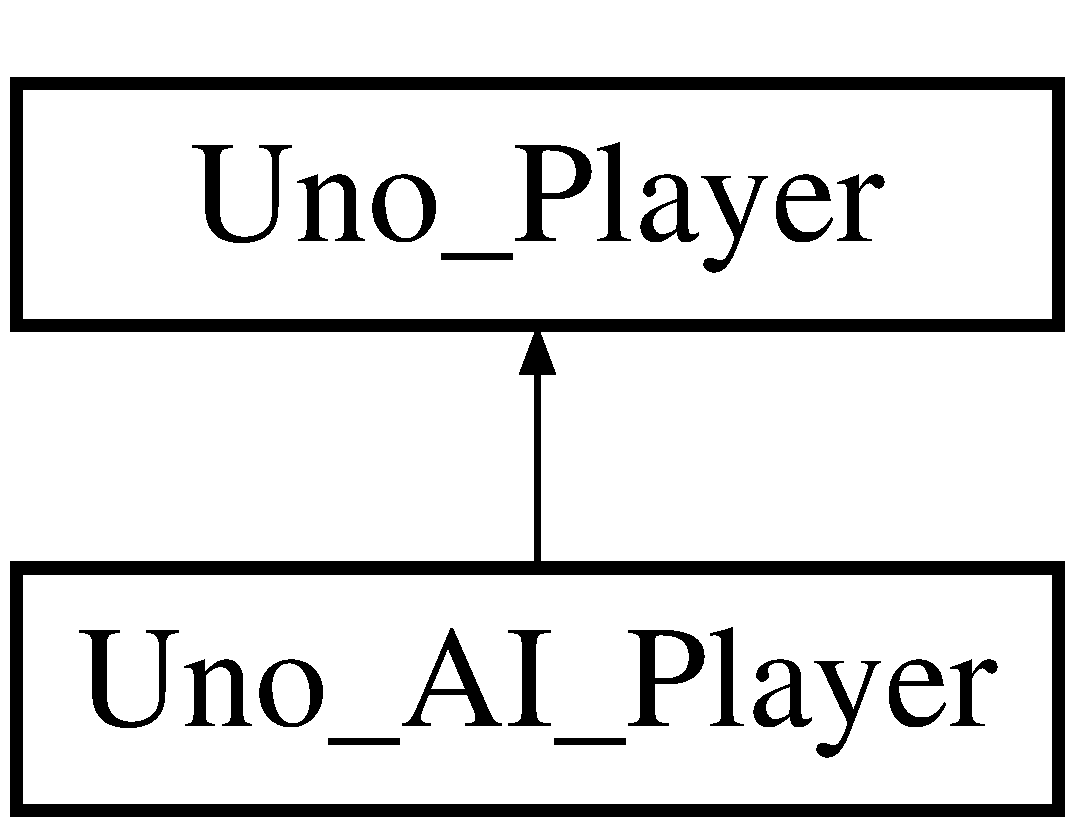
\includegraphics[height=2.000000cm]{class_uno___a_i___player}
\end{center}
\end{figure}
\subsection*{\-Public \-Member \-Functions}
\begin{DoxyCompactItemize}
\item 
\hyperlink{class_uno___a_i___player_ae977868f52c315663174b5c4943ac9ef}{\-Uno\-\_\-\-A\-I\-\_\-\-Player} ()
\begin{DoxyCompactList}\small\item\em \-Default constructor. \end{DoxyCompactList}\item 
\hyperlink{class_uno___a_i___player_ab16352005d98a759d298d05afdaaea9e}{\-Uno\-\_\-\-A\-I\-\_\-\-Player} (const string \&n, unsigned int s, unsigned int l)
\begin{DoxyCompactList}\small\item\em \-Full value specification constructor. \end{DoxyCompactList}\item 
\hyperlink{class_uno___action}{\-Uno\-\_\-\-Action} \hyperlink{class_uno___a_i___player_a46dd95e2b2ff44fa0b5cc80fb1d66605}{take\-\_\-turn} (const \hyperlink{class_uno___p_state}{\-Uno\-\_\-\-P\-State} \&s)
\begin{DoxyCompactList}\small\item\em \-Calls the player to take his turn. \end{DoxyCompactList}\end{DoxyCompactItemize}
\subsection*{\-Public \-Attributes}
\begin{DoxyCompactItemize}
\item 
unsigned char \hyperlink{class_uno___a_i___player_a028b0df8cca96eb10fc87bebf0f48c25}{m\-\_\-level}
\begin{DoxyCompactList}\small\item\em \-The player's \-A\-I difficulty level. \end{DoxyCompactList}\end{DoxyCompactItemize}


\subsection{\-Detailed \-Description}
\-An \-A\-I player for the game. 

\-This class is used to represent a computer player for an \-Uno game. 

\subsection{\-Constructor \& \-Destructor \-Documentation}
\hypertarget{class_uno___a_i___player_ae977868f52c315663174b5c4943ac9ef}{
\index{\-Uno\-\_\-\-A\-I\-\_\-\-Player@{\-Uno\-\_\-\-A\-I\-\_\-\-Player}!\-Uno\-\_\-\-A\-I\-\_\-\-Player@{\-Uno\-\_\-\-A\-I\-\_\-\-Player}}
\index{\-Uno\-\_\-\-A\-I\-\_\-\-Player@{\-Uno\-\_\-\-A\-I\-\_\-\-Player}!Uno_AI_Player@{\-Uno\-\_\-\-A\-I\-\_\-\-Player}}
\subsubsection[{\-Uno\-\_\-\-A\-I\-\_\-\-Player}]{\setlength{\rightskip}{0pt plus 5cm}\-Uno\-\_\-\-A\-I\-\_\-\-Player\-::\-Uno\-\_\-\-A\-I\-\_\-\-Player (
\begin{DoxyParamCaption}
{}
\end{DoxyParamCaption}
)\hspace{0.3cm}{\ttfamily  \mbox{[}inline\mbox{]}}}}
\label{class_uno___a_i___player_ae977868f52c315663174b5c4943ac9ef}


\-Default constructor. 

\-Constructs an \hyperlink{class_uno___a_i___player}{\-Uno\-\_\-\-A\-I\-\_\-\-Player} with empty and zero values. \hypertarget{class_uno___a_i___player_ab16352005d98a759d298d05afdaaea9e}{
\index{\-Uno\-\_\-\-A\-I\-\_\-\-Player@{\-Uno\-\_\-\-A\-I\-\_\-\-Player}!\-Uno\-\_\-\-A\-I\-\_\-\-Player@{\-Uno\-\_\-\-A\-I\-\_\-\-Player}}
\index{\-Uno\-\_\-\-A\-I\-\_\-\-Player@{\-Uno\-\_\-\-A\-I\-\_\-\-Player}!Uno_AI_Player@{\-Uno\-\_\-\-A\-I\-\_\-\-Player}}
\subsubsection[{\-Uno\-\_\-\-A\-I\-\_\-\-Player}]{\setlength{\rightskip}{0pt plus 5cm}\-Uno\-\_\-\-A\-I\-\_\-\-Player\-::\-Uno\-\_\-\-A\-I\-\_\-\-Player (
\begin{DoxyParamCaption}
\item[{const string \&}]{n, }
\item[{unsigned int}]{s, }
\item[{unsigned int}]{l}
\end{DoxyParamCaption}
)}}
\label{class_uno___a_i___player_ab16352005d98a759d298d05afdaaea9e}


\-Full value specification constructor. 

\-Constructs an \hyperlink{class_uno___a_i___player}{\-Uno\-\_\-\-A\-I\-\_\-\-Player} with the given values. 
\begin{DoxyParams}{\-Parameters}
{\em n} & \-The name of the \hyperlink{class_uno___a_i___player}{\-Uno\-\_\-\-A\-I\-\_\-\-Player}. \\
\hline
{\em s} & \-The score for the \hyperlink{class_uno___a_i___player}{\-Uno\-\_\-\-A\-I\-\_\-\-Player}. \\
\hline
{\em l} & \-The difficulty level for the \hyperlink{class_uno___a_i___player}{\-Uno\-\_\-\-A\-I\-\_\-\-Player}. \\
\hline
\end{DoxyParams}


\subsection{\-Member \-Function \-Documentation}
\hypertarget{class_uno___a_i___player_a46dd95e2b2ff44fa0b5cc80fb1d66605}{
\index{\-Uno\-\_\-\-A\-I\-\_\-\-Player@{\-Uno\-\_\-\-A\-I\-\_\-\-Player}!take\-\_\-turn@{take\-\_\-turn}}
\index{take\-\_\-turn@{take\-\_\-turn}!Uno_AI_Player@{\-Uno\-\_\-\-A\-I\-\_\-\-Player}}
\subsubsection[{take\-\_\-turn}]{\setlength{\rightskip}{0pt plus 5cm}{\bf \-Uno\-\_\-\-Action} \-Uno\-\_\-\-A\-I\-\_\-\-Player\-::take\-\_\-turn (
\begin{DoxyParamCaption}
\item[{const {\bf \-Uno\-\_\-\-P\-State} \&}]{s}
\end{DoxyParamCaption}
)}}
\label{class_uno___a_i___player_a46dd95e2b2ff44fa0b5cc80fb1d66605}


\-Calls the player to take his turn. 

\-This function is invoked by the \hyperlink{class_uno___runner}{\-Uno\-\_\-\-Runner} whenever it is this player's turn in the game. 
\begin{DoxyParams}{\-Parameters}
{\em s} & \-The state of the game as visible from this player's perspective. \\
\hline
\end{DoxyParams}

\begin{DoxyRetVals}{\-Return values}
{\em \hyperlink{class_uno___action}{\-Uno\-\_\-\-Action}} & \-The \hyperlink{class_uno___action}{\-Uno\-\_\-\-Action} the player chooses this turn. \\
\hline
\end{DoxyRetVals}


\-Reimplemented from \hyperlink{class_uno___player_aa6e4a3177c39ee2572250b2dd4400a43}{\-Uno\-\_\-\-Player}.



\subsection{\-Member \-Data \-Documentation}
\hypertarget{class_uno___a_i___player_a028b0df8cca96eb10fc87bebf0f48c25}{
\index{\-Uno\-\_\-\-A\-I\-\_\-\-Player@{\-Uno\-\_\-\-A\-I\-\_\-\-Player}!m\-\_\-level@{m\-\_\-level}}
\index{m\-\_\-level@{m\-\_\-level}!Uno_AI_Player@{\-Uno\-\_\-\-A\-I\-\_\-\-Player}}
\subsubsection[{m\-\_\-level}]{\setlength{\rightskip}{0pt plus 5cm}unsigned char {\bf \-Uno\-\_\-\-A\-I\-\_\-\-Player\-::m\-\_\-level}}}
\label{class_uno___a_i___player_a028b0df8cca96eb10fc87bebf0f48c25}


\-The player's \-A\-I difficulty level. 

\-The level of the \-A\-I represents its difficulty level. \-A higher value means that an \-A\-I player will make more intelligent plays and be harder to defeat. 

\-The documentation for this class was generated from the following files\-:\begin{DoxyCompactItemize}
\item 
\-C\-:/\-Users/\-Gary/\-Documents/\-School/my-\/random-\/cpp-\/libraries/trunk/projects/graduate/cs6364/semester\-\_\-project/semester\-\_\-project/\hyperlink{uno__ai__player_8h}{uno\-\_\-ai\-\_\-player.\-h}\item 
\-C\-:/\-Users/\-Gary/\-Documents/\-School/my-\/random-\/cpp-\/libraries/trunk/projects/graduate/cs6364/semester\-\_\-project/semester\-\_\-project/\hyperlink{uno__ai__player_8cpp}{uno\-\_\-ai\-\_\-player.\-cpp}\end{DoxyCompactItemize}

\hypertarget{class_uno___game___state}{
\section{\-Uno\-\_\-\-Game\-\_\-\-State \-Class \-Reference}
\label{class_uno___game___state}\index{\-Uno\-\_\-\-Game\-\_\-\-State@{\-Uno\-\_\-\-Game\-\_\-\-State}}
}


\-Holds the state of the game.  




{\ttfamily \#include $<$uno\-\_\-game\-\_\-state.\-h$>$}

\subsection*{\-Public \-Member \-Functions}
\begin{DoxyCompactItemize}
\item 
\hypertarget{class_uno___game___state_a8c17d72f7a46910c00e916e5df76f7f5}{
\hyperlink{class_uno___game___state_a8c17d72f7a46910c00e916e5df76f7f5}{\-Uno\-\_\-\-Game\-\_\-\-State} ()}
\label{class_uno___game___state_a8c17d72f7a46910c00e916e5df76f7f5}

\begin{DoxyCompactList}\small\item\em \-Default constructor, no values assigned. \end{DoxyCompactList}\end{DoxyCompactItemize}
\subsection*{\-Public \-Attributes}
\begin{DoxyCompactItemize}
\item 
\hypertarget{class_uno___game___state_adff61ccfa1552c4524e781aeee6ed95a}{
vector$<$ \hyperlink{class_uno___player}{\-Uno\-\_\-\-Player} $>$ \hyperlink{class_uno___game___state_adff61ccfa1552c4524e781aeee6ed95a}{m\-\_\-players}}
\label{class_uno___game___state_adff61ccfa1552c4524e781aeee6ed95a}

\begin{DoxyCompactList}\small\item\em \-The collection of players in this game. \end{DoxyCompactList}\item 
\hypertarget{class_uno___game___state_a85a2ea5d9e50359519aeeef2589fa8cf}{
unsigned int \hyperlink{class_uno___game___state_a85a2ea5d9e50359519aeeef2589fa8cf}{m\-\_\-turn}}
\label{class_uno___game___state_a85a2ea5d9e50359519aeeef2589fa8cf}

\begin{DoxyCompactList}\small\item\em \-The index of the player whose turn it is. \end{DoxyCompactList}\item 
\hypertarget{class_uno___game___state_abc3bb6447a74a7bf28c1dfbbfdcd6d55}{
unsigned int \hyperlink{class_uno___game___state_abc3bb6447a74a7bf28c1dfbbfdcd6d55}{m\-\_\-turn\-\_\-count}}
\label{class_uno___game___state_abc3bb6447a74a7bf28c1dfbbfdcd6d55}

\begin{DoxyCompactList}\small\item\em \-The turn count. \-The number of turns elapsed in the game. \end{DoxyCompactList}\item 
\hyperlink{uno__deck_8h_ab634a15f4d19d3af113a71241b79c408}{deck} \hyperlink{class_uno___game___state_a7bf61c252c9de176f309b691b4038345}{m\-\_\-unplayed}
\begin{DoxyCompactList}\small\item\em \-The unplayed deck of cards for this game. \end{DoxyCompactList}\item 
\hyperlink{uno__deck_8h_ab634a15f4d19d3af113a71241b79c408}{deck} \hyperlink{class_uno___game___state_ae274bd2383addaefbc78556c48757c35}{m\-\_\-played}
\begin{DoxyCompactList}\small\item\em \-The played deck of cards for this game. \end{DoxyCompactList}\item 
unsigned int \hyperlink{class_uno___game___state_ad55fa08fbfc6ddf4359194857dbd99fc}{m\-\_\-eval\-\_\-score}
\begin{DoxyCompactList}\small\item\em \-A heuristic score evaluation for this state for an \-A\-I player. \end{DoxyCompactList}\end{DoxyCompactItemize}


\subsection{\-Detailed \-Description}
\-Holds the state of the game. 

\-Includes the players, whose turn it is, the unplayed and played cards, and, for an \-A\-I player, the evaluation score of the state. 

\subsection{\-Member \-Data \-Documentation}
\hypertarget{class_uno___game___state_ad55fa08fbfc6ddf4359194857dbd99fc}{
\index{\-Uno\-\_\-\-Game\-\_\-\-State@{\-Uno\-\_\-\-Game\-\_\-\-State}!m\-\_\-eval\-\_\-score@{m\-\_\-eval\-\_\-score}}
\index{m\-\_\-eval\-\_\-score@{m\-\_\-eval\-\_\-score}!Uno_Game_State@{\-Uno\-\_\-\-Game\-\_\-\-State}}
\subsubsection[{m\-\_\-eval\-\_\-score}]{\setlength{\rightskip}{0pt plus 5cm}unsigned int {\bf \-Uno\-\_\-\-Game\-\_\-\-State\-::m\-\_\-eval\-\_\-score}}}
\label{class_uno___game___state_ad55fa08fbfc6ddf4359194857dbd99fc}


\-A heuristic score evaluation for this state for an \-A\-I player. 

\-This value is rather meaningless for a real player, but for an \-A\-I player this represents how \char`\"{}good\char`\"{} a state is. \-A state that represents a loss for the player whose turn it is will have an extremely low value. \hypertarget{class_uno___game___state_ae274bd2383addaefbc78556c48757c35}{
\index{\-Uno\-\_\-\-Game\-\_\-\-State@{\-Uno\-\_\-\-Game\-\_\-\-State}!m\-\_\-played@{m\-\_\-played}}
\index{m\-\_\-played@{m\-\_\-played}!Uno_Game_State@{\-Uno\-\_\-\-Game\-\_\-\-State}}
\subsubsection[{m\-\_\-played}]{\setlength{\rightskip}{0pt plus 5cm}{\bf deck} {\bf \-Uno\-\_\-\-Game\-\_\-\-State\-::m\-\_\-played}}}
\label{class_uno___game___state_ae274bd2383addaefbc78556c48757c35}


\-The played deck of cards for this game. 

\-When a player plays a card it is placed on top of this deck. \hypertarget{class_uno___game___state_a7bf61c252c9de176f309b691b4038345}{
\index{\-Uno\-\_\-\-Game\-\_\-\-State@{\-Uno\-\_\-\-Game\-\_\-\-State}!m\-\_\-unplayed@{m\-\_\-unplayed}}
\index{m\-\_\-unplayed@{m\-\_\-unplayed}!Uno_Game_State@{\-Uno\-\_\-\-Game\-\_\-\-State}}
\subsubsection[{m\-\_\-unplayed}]{\setlength{\rightskip}{0pt plus 5cm}{\bf deck} {\bf \-Uno\-\_\-\-Game\-\_\-\-State\-::m\-\_\-unplayed}}}
\label{class_uno___game___state_a7bf61c252c9de176f309b691b4038345}


\-The unplayed deck of cards for this game. 

\-When a player draws a card it comes from the top of this deck. 

\-The documentation for this class was generated from the following files\-:\begin{DoxyCompactItemize}
\item 
\-C\-:/\-Users/\-Gary/\-Documents/\-School/my-\/random-\/cpp-\/libraries/trunk/projects/graduate/cs6364/semester\-\_\-project/semester\-\_\-project/\hyperlink{uno__game__state_8h}{uno\-\_\-game\-\_\-state.\-h}\item 
\-C\-:/\-Users/\-Gary/\-Documents/\-School/my-\/random-\/cpp-\/libraries/trunk/projects/graduate/cs6364/semester\-\_\-project/semester\-\_\-project/\hyperlink{uno__game__state_8cpp}{uno\-\_\-game\-\_\-state.\-cpp}\end{DoxyCompactItemize}

\hypertarget{class_uno___human___player}{
\section{\-Uno\-\_\-\-Human\-\_\-\-Player \-Class \-Reference}
\label{class_uno___human___player}\index{\-Uno\-\_\-\-Human\-\_\-\-Player@{\-Uno\-\_\-\-Human\-\_\-\-Player}}
}


\-A human player for the game.  




{\ttfamily \#include $<$uno\-\_\-human\-\_\-player.\-h$>$}

\-Inheritance diagram for \-Uno\-\_\-\-Human\-\_\-\-Player\-:\begin{figure}[H]
\begin{center}
\leavevmode
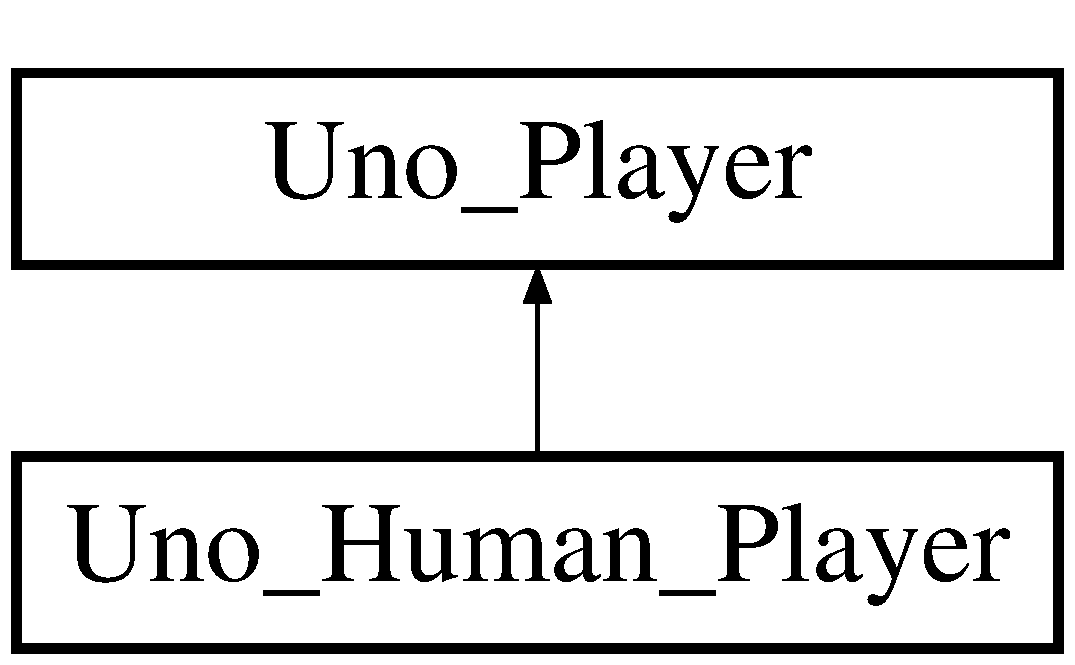
\includegraphics[height=2.000000cm]{class_uno___human___player}
\end{center}
\end{figure}
\subsection*{\-Public \-Member \-Functions}
\begin{DoxyCompactItemize}
\item 
\hyperlink{class_uno___human___player_a7339947e9ae326b26ccd478c2aa23664}{\-Uno\-\_\-\-Human\-\_\-\-Player} ()
\begin{DoxyCompactList}\small\item\em \-Default constructor. \end{DoxyCompactList}\item 
\hyperlink{class_uno___human___player_a126f7617c19e1ff7ca5db185b5b47735}{\-Uno\-\_\-\-Human\-\_\-\-Player} (const string \&n, unsigned int s)
\begin{DoxyCompactList}\small\item\em \-Full value specification constructor. \end{DoxyCompactList}\item 
\hyperlink{class_uno___action}{\-Uno\-\_\-\-Action} \hyperlink{class_uno___human___player_a14a73bddb4791cc7406a0e9cfe65979b}{take\-\_\-turn} (const \hyperlink{class_uno___p_state}{\-Uno\-\_\-\-P\-State} \&s)
\begin{DoxyCompactList}\small\item\em \-Calls the player to take his turn. \end{DoxyCompactList}\end{DoxyCompactItemize}


\subsection{\-Detailed \-Description}
\-A human player for the game. 

\-This class is used to represent a human player for an \-Uno game. 

\subsection{\-Constructor \& \-Destructor \-Documentation}
\hypertarget{class_uno___human___player_a7339947e9ae326b26ccd478c2aa23664}{
\index{\-Uno\-\_\-\-Human\-\_\-\-Player@{\-Uno\-\_\-\-Human\-\_\-\-Player}!\-Uno\-\_\-\-Human\-\_\-\-Player@{\-Uno\-\_\-\-Human\-\_\-\-Player}}
\index{\-Uno\-\_\-\-Human\-\_\-\-Player@{\-Uno\-\_\-\-Human\-\_\-\-Player}!Uno_Human_Player@{\-Uno\-\_\-\-Human\-\_\-\-Player}}
\subsubsection[{\-Uno\-\_\-\-Human\-\_\-\-Player}]{\setlength{\rightskip}{0pt plus 5cm}\-Uno\-\_\-\-Human\-\_\-\-Player\-::\-Uno\-\_\-\-Human\-\_\-\-Player (
\begin{DoxyParamCaption}
{}
\end{DoxyParamCaption}
)\hspace{0.3cm}{\ttfamily  \mbox{[}inline\mbox{]}}}}
\label{class_uno___human___player_a7339947e9ae326b26ccd478c2aa23664}


\-Default constructor. 

\-Constructs an \hyperlink{class_uno___human___player}{\-Uno\-\_\-\-Human\-\_\-\-Player} with empty and zero values. \hypertarget{class_uno___human___player_a126f7617c19e1ff7ca5db185b5b47735}{
\index{\-Uno\-\_\-\-Human\-\_\-\-Player@{\-Uno\-\_\-\-Human\-\_\-\-Player}!\-Uno\-\_\-\-Human\-\_\-\-Player@{\-Uno\-\_\-\-Human\-\_\-\-Player}}
\index{\-Uno\-\_\-\-Human\-\_\-\-Player@{\-Uno\-\_\-\-Human\-\_\-\-Player}!Uno_Human_Player@{\-Uno\-\_\-\-Human\-\_\-\-Player}}
\subsubsection[{\-Uno\-\_\-\-Human\-\_\-\-Player}]{\setlength{\rightskip}{0pt plus 5cm}\-Uno\-\_\-\-Human\-\_\-\-Player\-::\-Uno\-\_\-\-Human\-\_\-\-Player (
\begin{DoxyParamCaption}
\item[{const string \&}]{n, }
\item[{unsigned int}]{s}
\end{DoxyParamCaption}
)}}
\label{class_uno___human___player_a126f7617c19e1ff7ca5db185b5b47735}


\-Full value specification constructor. 

\-Constructs an \hyperlink{class_uno___human___player}{\-Uno\-\_\-\-Human\-\_\-\-Player} with the given values. 
\begin{DoxyParams}{\-Parameters}
{\em n} & \-The name of the \hyperlink{class_uno___human___player}{\-Uno\-\_\-\-Human\-\_\-\-Player}. \\
\hline
{\em s} & \-The score for the \hyperlink{class_uno___human___player}{\-Uno\-\_\-\-Human\-\_\-\-Player}. \\
\hline
\end{DoxyParams}


\subsection{\-Member \-Function \-Documentation}
\hypertarget{class_uno___human___player_a14a73bddb4791cc7406a0e9cfe65979b}{
\index{\-Uno\-\_\-\-Human\-\_\-\-Player@{\-Uno\-\_\-\-Human\-\_\-\-Player}!take\-\_\-turn@{take\-\_\-turn}}
\index{take\-\_\-turn@{take\-\_\-turn}!Uno_Human_Player@{\-Uno\-\_\-\-Human\-\_\-\-Player}}
\subsubsection[{take\-\_\-turn}]{\setlength{\rightskip}{0pt plus 5cm}{\bf \-Uno\-\_\-\-Action} \-Uno\-\_\-\-Human\-\_\-\-Player\-::take\-\_\-turn (
\begin{DoxyParamCaption}
\item[{const {\bf \-Uno\-\_\-\-P\-State} \&}]{s}
\end{DoxyParamCaption}
)}}
\label{class_uno___human___player_a14a73bddb4791cc7406a0e9cfe65979b}


\-Calls the player to take his turn. 

\-This function is invoked by the \hyperlink{class_uno___runner}{\-Uno\-\_\-\-Runner} whenever it is this player's turn in the game. 
\begin{DoxyParams}{\-Parameters}
{\em s} & \-The state of the game as visible from this player's perspective. \\
\hline
\end{DoxyParams}

\begin{DoxyRetVals}{\-Return values}
{\em \hyperlink{class_uno___action}{\-Uno\-\_\-\-Action}} & \-The \hyperlink{class_uno___action}{\-Uno\-\_\-\-Action} the player chooses this turn. \\
\hline
\end{DoxyRetVals}


\-Reimplemented from \hyperlink{class_uno___player_aa6e4a3177c39ee2572250b2dd4400a43}{\-Uno\-\_\-\-Player}.



\-The documentation for this class was generated from the following files\-:\begin{DoxyCompactItemize}
\item 
\-C\-:/\-Users/\-Gary/\-Documents/\-School/my-\/random-\/cpp-\/libraries/trunk/projects/graduate/cs6364/semester\-\_\-project/semester\-\_\-project/\hyperlink{uno__human__player_8h}{uno\-\_\-human\-\_\-player.\-h}\item 
\-C\-:/\-Users/\-Gary/\-Documents/\-School/my-\/random-\/cpp-\/libraries/trunk/projects/graduate/cs6364/semester\-\_\-project/semester\-\_\-project/\hyperlink{uno__human__player_8cpp}{uno\-\_\-human\-\_\-player.\-cpp}\end{DoxyCompactItemize}

\hypertarget{class_uno___player}{
\section{\-Uno\-\_\-\-Player \-Class \-Reference}
\label{class_uno___player}\index{\-Uno\-\_\-\-Player@{\-Uno\-\_\-\-Player}}
}


\-Models a real player for the game.  




{\ttfamily \#include $<$uno\-\_\-player.\-h$>$}

\-Inheritance diagram for \-Uno\-\_\-\-Player\-:\begin{figure}[H]
\begin{center}
\leavevmode
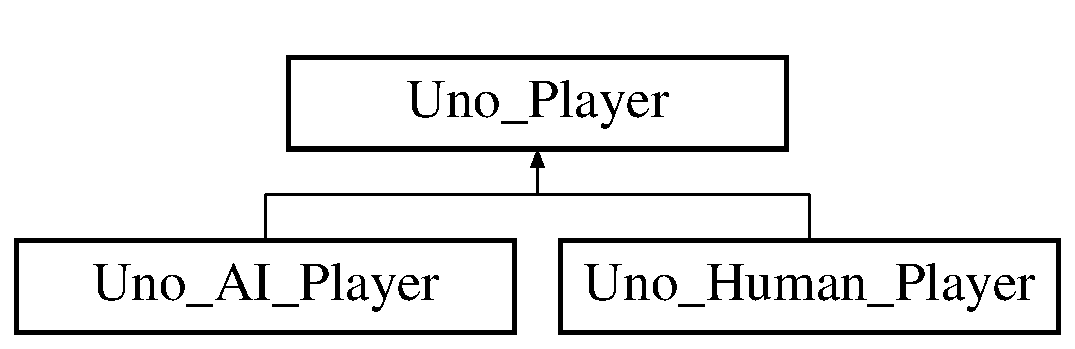
\includegraphics[height=2.000000cm]{class_uno___player}
\end{center}
\end{figure}
\subsection*{\-Public \-Member \-Functions}
\begin{DoxyCompactItemize}
\item 
\hyperlink{class_uno___player_a0447ff92b80be8d98d0052d7d2a868d7}{\-Uno\-\_\-\-Player} ()
\begin{DoxyCompactList}\small\item\em \-Default constructor. \end{DoxyCompactList}\item 
\hyperlink{class_uno___player_a01b27e59f1de1e13627c2e72e69c65c6}{\-Uno\-\_\-\-Player} (const string \&n, unsigned int s)
\begin{DoxyCompactList}\small\item\em \-Identification constructor. \end{DoxyCompactList}\item 
\hyperlink{class_uno___player_acd18cd073963d561da37018f114ef29b}{\-Uno\-\_\-\-Player} (const \hyperlink{uno__player_8h_acd9523c15e47a87e3740cf5ade73556e}{hand} \&h, const string \&n, unsigned int s)
\begin{DoxyCompactList}\small\item\em \-Full value specification constructor. \end{DoxyCompactList}\item 
void \hyperlink{class_uno___player_ac803ffaaf0efeaa27d3d4993545bee39}{draw\-\_\-card} (\hyperlink{uno__deck_8h_ab634a15f4d19d3af113a71241b79c408}{deck} \&d)
\begin{DoxyCompactList}\small\item\em \-Draws a card from the deck and puts it in the player's hand. \end{DoxyCompactList}\item 
void \hyperlink{class_uno___player_a5f0d9630e8e143f34c4d63340bac90e0}{draw\-\_\-initial\-\_\-hand} (\hyperlink{uno__deck_8h_ab634a15f4d19d3af113a71241b79c408}{deck} \&d)
\begin{DoxyCompactList}\small\item\em \-Draws \-U\-N\-O\-\_\-\-I\-N\-I\-T\-\_\-\-H\-A\-N\-D\-\_\-\-S\-I\-Z\-E cards from the deck and puts them in the player's hand. \end{DoxyCompactList}\item 
\hyperlink{uno__card_8h_ab16a632e2e3f1f154cce75648902eb83}{card} \hyperlink{class_uno___player_a2e94c703cf4f680c4dcbcb1adbb4816b}{play\-\_\-card\-\_\-by\-\_\-name} (\hyperlink{uno__card_8h_ab16a632e2e3f1f154cce75648902eb83}{card} c)
\begin{DoxyCompactList}\small\item\em \-Plays a card with the given name from the player's hand. \end{DoxyCompactList}\item 
\hyperlink{uno__card_8h_ab16a632e2e3f1f154cce75648902eb83}{card} \hyperlink{class_uno___player_abe1a86f4792fa9e703ffeb28e453160f}{play\-\_\-card\-\_\-by\-\_\-index} (unsigned char i)
\begin{DoxyCompactList}\small\item\em \-Plays a card at the given index from the player's hand. \end{DoxyCompactList}\item 
void \hyperlink{class_uno___player_a3af4557fcf900bc6357000449ecb5860}{print\-\_\-hand} ()
\begin{DoxyCompactList}\small\item\em \-Prints out this player's hand of cards. \end{DoxyCompactList}\item 
void \hyperlink{class_uno___player_a17a542fc645418ee806c79ebe253a62e}{print\-\_\-hand\-\_\-values} ()
\begin{DoxyCompactList}\small\item\em \-Prints out the values of this player's hand of cards. \end{DoxyCompactList}\end{DoxyCompactItemize}
\subsection*{\-Public \-Attributes}
\begin{DoxyCompactItemize}
\item 
\hyperlink{uno__player_8h_acd9523c15e47a87e3740cf5ade73556e}{hand} \hyperlink{class_uno___player_a9d50084b9fd4b005286ffdaa004f2664}{m\-\_\-hand}
\begin{DoxyCompactList}\small\item\em \-The player's hand of cards. \end{DoxyCompactList}\item 
string \hyperlink{class_uno___player_a06af109b4d621efa14ba98e4c9395739}{m\-\_\-name}
\begin{DoxyCompactList}\small\item\em \-The player's name. \end{DoxyCompactList}\item 
unsigned int \hyperlink{class_uno___player_a9805f306a500b1898c0a0922d76de444}{m\-\_\-score}
\begin{DoxyCompactList}\small\item\em \-The player's score. \end{DoxyCompactList}\end{DoxyCompactItemize}


\subsection{\-Detailed \-Description}
\-Models a real player for the game. 

\subsection{\-Constructor \& \-Destructor \-Documentation}
\hypertarget{class_uno___player_a0447ff92b80be8d98d0052d7d2a868d7}{
\index{\-Uno\-\_\-\-Player@{\-Uno\-\_\-\-Player}!\-Uno\-\_\-\-Player@{\-Uno\-\_\-\-Player}}
\index{\-Uno\-\_\-\-Player@{\-Uno\-\_\-\-Player}!Uno_Player@{\-Uno\-\_\-\-Player}}
\subsubsection[{\-Uno\-\_\-\-Player}]{\setlength{\rightskip}{0pt plus 5cm}\-Uno\-\_\-\-Player\-::\-Uno\-\_\-\-Player (
\begin{DoxyParamCaption}
{}
\end{DoxyParamCaption}
)}}
\label{class_uno___player_a0447ff92b80be8d98d0052d7d2a868d7}


\-Default constructor. 

\-Constructs an \hyperlink{class_uno___player}{\-Uno\-\_\-\-Player} with an empty hand, a blank name, and score and level of zero. \hypertarget{class_uno___player_a01b27e59f1de1e13627c2e72e69c65c6}{
\index{\-Uno\-\_\-\-Player@{\-Uno\-\_\-\-Player}!\-Uno\-\_\-\-Player@{\-Uno\-\_\-\-Player}}
\index{\-Uno\-\_\-\-Player@{\-Uno\-\_\-\-Player}!Uno_Player@{\-Uno\-\_\-\-Player}}
\subsubsection[{\-Uno\-\_\-\-Player}]{\setlength{\rightskip}{0pt plus 5cm}\-Uno\-\_\-\-Player\-::\-Uno\-\_\-\-Player (
\begin{DoxyParamCaption}
\item[{const string \&}]{n, }
\item[{unsigned int}]{s}
\end{DoxyParamCaption}
)}}
\label{class_uno___player_a01b27e59f1de1e13627c2e72e69c65c6}


\-Identification constructor. 

\-Constructs an \hyperlink{class_uno___player}{\-Uno\-\_\-\-Player} with an with the given name, score, and level. \hypertarget{class_uno___player_acd18cd073963d561da37018f114ef29b}{
\index{\-Uno\-\_\-\-Player@{\-Uno\-\_\-\-Player}!\-Uno\-\_\-\-Player@{\-Uno\-\_\-\-Player}}
\index{\-Uno\-\_\-\-Player@{\-Uno\-\_\-\-Player}!Uno_Player@{\-Uno\-\_\-\-Player}}
\subsubsection[{\-Uno\-\_\-\-Player}]{\setlength{\rightskip}{0pt plus 5cm}\-Uno\-\_\-\-Player\-::\-Uno\-\_\-\-Player (
\begin{DoxyParamCaption}
\item[{const {\bf hand} \&}]{h, }
\item[{const string \&}]{n, }
\item[{unsigned int}]{s}
\end{DoxyParamCaption}
)}}
\label{class_uno___player_acd18cd073963d561da37018f114ef29b}


\-Full value specification constructor. 

\-Constructs an \hyperlink{class_uno___player}{\-Uno\-\_\-\-Player} with an with the given hand, name, score, and level. 

\subsection{\-Member \-Function \-Documentation}
\hypertarget{class_uno___player_ac803ffaaf0efeaa27d3d4993545bee39}{
\index{\-Uno\-\_\-\-Player@{\-Uno\-\_\-\-Player}!draw\-\_\-card@{draw\-\_\-card}}
\index{draw\-\_\-card@{draw\-\_\-card}!Uno_Player@{\-Uno\-\_\-\-Player}}
\subsubsection[{draw\-\_\-card}]{\setlength{\rightskip}{0pt plus 5cm}void \-Uno\-\_\-\-Player\-::draw\-\_\-card (
\begin{DoxyParamCaption}
\item[{{\bf deck} \&}]{d}
\end{DoxyParamCaption}
)}}
\label{class_uno___player_ac803ffaaf0efeaa27d3d4993545bee39}


\-Draws a card from the deck and puts it in the player's hand. 


\begin{DoxyParams}{\-Parameters}
{\em d} & \-The deck to draw a card from.\\
\hline
\end{DoxyParams}
\-Takes the top card from the deck and places it into the player's hand. \-The deck's size is decreased by one and the player's hand size is increased by one. \hypertarget{class_uno___player_a5f0d9630e8e143f34c4d63340bac90e0}{
\index{\-Uno\-\_\-\-Player@{\-Uno\-\_\-\-Player}!draw\-\_\-initial\-\_\-hand@{draw\-\_\-initial\-\_\-hand}}
\index{draw\-\_\-initial\-\_\-hand@{draw\-\_\-initial\-\_\-hand}!Uno_Player@{\-Uno\-\_\-\-Player}}
\subsubsection[{draw\-\_\-initial\-\_\-hand}]{\setlength{\rightskip}{0pt plus 5cm}void \-Uno\-\_\-\-Player\-::draw\-\_\-initial\-\_\-hand (
\begin{DoxyParamCaption}
\item[{{\bf deck} \&}]{d}
\end{DoxyParamCaption}
)}}
\label{class_uno___player_a5f0d9630e8e143f34c4d63340bac90e0}


\-Draws \-U\-N\-O\-\_\-\-I\-N\-I\-T\-\_\-\-H\-A\-N\-D\-\_\-\-S\-I\-Z\-E cards from the deck and puts them in the player's hand. 

\begin{DoxyPrecond}{\-Precondition}
d.\-size() $>$= \-U\-N\-O\-\_\-\-I\-N\-I\-T\-\_\-\-H\-A\-N\-D\-\_\-\-S\-I\-Z\-E 
\end{DoxyPrecond}

\begin{DoxyParams}{\-Parameters}
{\em d} & \-The deck to draw a card from.\\
\hline
\end{DoxyParams}
\-Takes the \-U\-N\-O\-\_\-\-I\-N\-I\-T\-\_\-\-H\-A\-N\-D\-\_\-\-S\-I\-Z\-E cards from the deck and places it into the player's hand. \-The deck's size is decreased by \-U\-N\-O\-\_\-\-I\-N\-I\-T\-\_\-\-H\-A\-N\-D\-\_\-\-S\-I\-Z\-E and the player's hand size is increased \-U\-N\-O\-\_\-\-I\-N\-I\-T\-\_\-\-H\-A\-N\-D\-\_\-\-S\-I\-Z\-E. \hypertarget{class_uno___player_abe1a86f4792fa9e703ffeb28e453160f}{
\index{\-Uno\-\_\-\-Player@{\-Uno\-\_\-\-Player}!play\-\_\-card\-\_\-by\-\_\-index@{play\-\_\-card\-\_\-by\-\_\-index}}
\index{play\-\_\-card\-\_\-by\-\_\-index@{play\-\_\-card\-\_\-by\-\_\-index}!Uno_Player@{\-Uno\-\_\-\-Player}}
\subsubsection[{play\-\_\-card\-\_\-by\-\_\-index}]{\setlength{\rightskip}{0pt plus 5cm}{\bf card} \-Uno\-\_\-\-Player\-::play\-\_\-card\-\_\-by\-\_\-index (
\begin{DoxyParamCaption}
\item[{unsigned char}]{i}
\end{DoxyParamCaption}
)}}
\label{class_uno___player_abe1a86f4792fa9e703ffeb28e453160f}


\-Plays a card at the given index from the player's hand. 

\begin{DoxyPrecond}{\-Precondition}
0 $<$= i $<$ m\-\_\-hand.\-size() 
\end{DoxyPrecond}

\begin{DoxyParams}{\-Parameters}
{\em i} & \-The index of the card in the player's hand to play. \\
\hline
\end{DoxyParams}
\begin{DoxyReturn}{\-Returns}
\-The card played.
\end{DoxyReturn}
\-Takes a card at index i and returns it. \-The card at index i is removed from the player's hand.

\begin{DoxyNote}{\-Note}
\-This is the preferred version of playing a card, as it is faster. 
\end{DoxyNote}
\hypertarget{class_uno___player_a2e94c703cf4f680c4dcbcb1adbb4816b}{
\index{\-Uno\-\_\-\-Player@{\-Uno\-\_\-\-Player}!play\-\_\-card\-\_\-by\-\_\-name@{play\-\_\-card\-\_\-by\-\_\-name}}
\index{play\-\_\-card\-\_\-by\-\_\-name@{play\-\_\-card\-\_\-by\-\_\-name}!Uno_Player@{\-Uno\-\_\-\-Player}}
\subsubsection[{play\-\_\-card\-\_\-by\-\_\-name}]{\setlength{\rightskip}{0pt plus 5cm}{\bf card} \-Uno\-\_\-\-Player\-::play\-\_\-card\-\_\-by\-\_\-name (
\begin{DoxyParamCaption}
\item[{{\bf card}}]{c}
\end{DoxyParamCaption}
)}}
\label{class_uno___player_a2e94c703cf4f680c4dcbcb1adbb4816b}


\-Plays a card with the given name from the player's hand. 


\begin{DoxyParams}{\-Parameters}
{\em c} & \-The card to play. \-To specify this name, use \-C\-A\-R\-D. \\
\hline
\end{DoxyParams}
\begin{DoxyReturn}{\-Returns}
\-The card played. \-If the specified card, c, does not exist in the player's hand, the card \hyperlink{uno__card_8h_abbc97b38c028c37643c949a6751283b7}{\-C\-A\-R\-D(\-U\-N\-O\-\_\-\-N\-O\-\_\-\-C\-O\-L\-O\-R, U\-N\-O\-\_\-\-R\-E\-S\-E\-R\-V\-E\-D)} is returned. 
\end{DoxyReturn}
\begin{DoxySeeAlso}{\-See also}
\hyperlink{uno__card_8h_abbc97b38c028c37643c949a6751283b7}{\-C\-A\-R\-D}
\end{DoxySeeAlso}
\-Takes a card specified by c and returns it. \-The card c is removed from the player's hand.

\-This version of play\-\_\-card is much less efficient than the index version. \begin{DoxySeeAlso}{\-See also}
\hyperlink{class_uno___player_abe1a86f4792fa9e703ffeb28e453160f}{play\-\_\-card\-\_\-by\-\_\-index( unsigned char i )} 
\end{DoxySeeAlso}
\hypertarget{class_uno___player_a3af4557fcf900bc6357000449ecb5860}{
\index{\-Uno\-\_\-\-Player@{\-Uno\-\_\-\-Player}!print\-\_\-hand@{print\-\_\-hand}}
\index{print\-\_\-hand@{print\-\_\-hand}!Uno_Player@{\-Uno\-\_\-\-Player}}
\subsubsection[{print\-\_\-hand}]{\setlength{\rightskip}{0pt plus 5cm}void \-Uno\-\_\-\-Player\-::print\-\_\-hand (
\begin{DoxyParamCaption}
{}
\end{DoxyParamCaption}
)}}
\label{class_uno___player_a3af4557fcf900bc6357000449ecb5860}


\-Prints out this player's hand of cards. 

\begin{DoxySeeAlso}{\-See also}
typedef vector$<$card$>$ \hyperlink{uno__deck_8h_ab634a15f4d19d3af113a71241b79c408}{deck} 
\end{DoxySeeAlso}
\begin{DoxyNote}{\-Note}
\-This is a relatively expensive operation, use sparingly. 
\end{DoxyNote}
\hypertarget{class_uno___player_a17a542fc645418ee806c79ebe253a62e}{
\index{\-Uno\-\_\-\-Player@{\-Uno\-\_\-\-Player}!print\-\_\-hand\-\_\-values@{print\-\_\-hand\-\_\-values}}
\index{print\-\_\-hand\-\_\-values@{print\-\_\-hand\-\_\-values}!Uno_Player@{\-Uno\-\_\-\-Player}}
\subsubsection[{print\-\_\-hand\-\_\-values}]{\setlength{\rightskip}{0pt plus 5cm}void \-Uno\-\_\-\-Player\-::print\-\_\-hand\-\_\-values (
\begin{DoxyParamCaption}
{}
\end{DoxyParamCaption}
)}}
\label{class_uno___player_a17a542fc645418ee806c79ebe253a62e}


\-Prints out the values of this player's hand of cards. 

\begin{DoxySeeAlso}{\-See also}
typedef vector$<$card$>$ \hyperlink{uno__deck_8h_ab634a15f4d19d3af113a71241b79c408}{deck} 
\end{DoxySeeAlso}
\begin{DoxyNote}{\-Note}
\-This is a less expensive operation than \hyperlink{class_uno___player_a3af4557fcf900bc6357000449ecb5860}{print\-\_\-hand()} but is still relatively expensive, use sparingly. 
\end{DoxyNote}


\subsection{\-Member \-Data \-Documentation}
\hypertarget{class_uno___player_a9d50084b9fd4b005286ffdaa004f2664}{
\index{\-Uno\-\_\-\-Player@{\-Uno\-\_\-\-Player}!m\-\_\-hand@{m\-\_\-hand}}
\index{m\-\_\-hand@{m\-\_\-hand}!Uno_Player@{\-Uno\-\_\-\-Player}}
\subsubsection[{m\-\_\-hand}]{\setlength{\rightskip}{0pt plus 5cm}{\bf hand} {\bf \-Uno\-\_\-\-Player\-::m\-\_\-hand}}}
\label{class_uno___player_a9d50084b9fd4b005286ffdaa004f2664}


\-The player's hand of cards. 

\-The player's hand of cards is initially 7 cards drawn from a deck. \hypertarget{class_uno___player_a06af109b4d621efa14ba98e4c9395739}{
\index{\-Uno\-\_\-\-Player@{\-Uno\-\_\-\-Player}!m\-\_\-name@{m\-\_\-name}}
\index{m\-\_\-name@{m\-\_\-name}!Uno_Player@{\-Uno\-\_\-\-Player}}
\subsubsection[{m\-\_\-name}]{\setlength{\rightskip}{0pt plus 5cm}string {\bf \-Uno\-\_\-\-Player\-::m\-\_\-name}}}
\label{class_uno___player_a06af109b4d621efa14ba98e4c9395739}


\-The player's name. 

\-A string representing the player's name. \hypertarget{class_uno___player_a9805f306a500b1898c0a0922d76de444}{
\index{\-Uno\-\_\-\-Player@{\-Uno\-\_\-\-Player}!m\-\_\-score@{m\-\_\-score}}
\index{m\-\_\-score@{m\-\_\-score}!Uno_Player@{\-Uno\-\_\-\-Player}}
\subsubsection[{m\-\_\-score}]{\setlength{\rightskip}{0pt plus 5cm}unsigned int {\bf \-Uno\-\_\-\-Player\-::m\-\_\-score}}}
\label{class_uno___player_a9805f306a500b1898c0a0922d76de444}


\-The player's score. 

\-Each player attains a number of points at the end of each game. \-The point total for a player is tracked using this. \begin{DoxyNote}{\-Note}
\-The first player to reach 500 points in a regulation game is considered the winner. 
\end{DoxyNote}


\-The documentation for this class was generated from the following files\-:\begin{DoxyCompactItemize}
\item 
\-C\-:/\-Users/\-Gary/\-Documents/\-School/my-\/random-\/cpp-\/libraries/trunk/projects/graduate/cs6364/semester\-\_\-project/semester\-\_\-project/\hyperlink{uno__player_8h}{uno\-\_\-player.\-h}\item 
\-C\-:/\-Users/\-Gary/\-Documents/\-School/my-\/random-\/cpp-\/libraries/trunk/projects/graduate/cs6364/semester\-\_\-project/semester\-\_\-project/\hyperlink{uno__player_8cpp}{uno\-\_\-player.\-cpp}\end{DoxyCompactItemize}

\hypertarget{class_uno___runner}{
\section{\-Uno\-\_\-\-Runner \-Class \-Reference}
\label{class_uno___runner}\index{\-Uno\-\_\-\-Runner@{\-Uno\-\_\-\-Runner}}
}


\-Runs an \-Uno game.  




{\ttfamily \#include $<$uno\-\_\-runner.\-h$>$}

\subsection*{\-Public \-Member \-Functions}
\begin{DoxyCompactItemize}
\item 
\hypertarget{class_uno___runner_a485bf9506331363e4b0d6208ee446497}{
\hyperlink{class_uno___runner_a485bf9506331363e4b0d6208ee446497}{\-Uno\-\_\-\-Runner} ()}
\label{class_uno___runner_a485bf9506331363e4b0d6208ee446497}

\begin{DoxyCompactList}\small\item\em \-Default constructor. \-Does nothing. \end{DoxyCompactList}\item 
bool \hyperlink{class_uno___runner_ae015517f7d4493ddbaaeacd98be0b9b8}{setup} ()
\begin{DoxyCompactList}\small\item\em \-Sets up a game to be played. \end{DoxyCompactList}\item 
bool \hyperlink{class_uno___runner_a982f614c5afa8faa57aedc3116f3d237}{add\-\_\-player} (const \hyperlink{class_uno___player}{\-Uno\-\_\-\-Player} \&p)
\begin{DoxyCompactList}\small\item\em \-Adds player p to the game if possible. \end{DoxyCompactList}\item 
bool \hyperlink{class_uno___runner_acae1277934b338e4c6edd8d45eea5a3e}{remove\-\_\-player} (unsigned char i, unsigned char c=0)
\begin{DoxyCompactList}\small\item\em \-Removes player i from the game if possible. \end{DoxyCompactList}\item 
unsigned int \hyperlink{class_uno___runner_aa3f43b6ab9042ff74a34ad3fae8a0b11}{num\-\_\-players} ()
\begin{DoxyCompactList}\small\item\em \-Returns the number of players in the game. \end{DoxyCompactList}\item 
void \hyperlink{class_uno___runner_a79c386fc295240e53b20c1270f31ab41}{set\-\_\-unplayed\-\_\-deck} (const \hyperlink{uno__deck_8h_ab634a15f4d19d3af113a71241b79c408}{deck} \&d)
\begin{DoxyCompactList}\small\item\em \-Sets the unplayed deck to use for the game. \end{DoxyCompactList}\item 
void \hyperlink{class_uno___runner_ac98c68091701dcf1deeaad7a5168dec8}{set\-\_\-played\-\_\-deck} (const \hyperlink{uno__deck_8h_ab634a15f4d19d3af113a71241b79c408}{deck} \&d)
\begin{DoxyCompactList}\small\item\em \-Sets the played deck to use for the game. \end{DoxyCompactList}\item 
void \hyperlink{class_uno___runner_a885e7ac58c656e1cb0bc4e49cd494874}{print\-\_\-played} (unsigned char f)
\begin{DoxyCompactList}\small\item\em \-Prints out the stack of played cards to the screen. \end{DoxyCompactList}\item 
void \hyperlink{class_uno___runner_a53b830015937722abd8ec515405534f9}{print\-\_\-unplayed} (unsigned char f)
\begin{DoxyCompactList}\small\item\em \-Prints out the stack of unplayed cards to the screen. \end{DoxyCompactList}\item 
void \hyperlink{class_uno___runner_a2d16089c5bdf20c1120be067797a349a}{print\-\_\-state} ()
\begin{DoxyCompactList}\small\item\em \-Prints out the state of the game. \-This includes\-: \end{DoxyCompactList}\item 
void \hyperlink{class_uno___runner_a3f0847989a9868bcd023b41ee5f28d0a}{run} ()
\begin{DoxyCompactList}\small\item\em \-Runs the \-Uno game. \end{DoxyCompactList}\end{DoxyCompactItemize}


\subsection{\-Detailed \-Description}
\-Runs an \-Uno game. 

\-To actually play a game of \-Uno using the \-A\-I, create an object of this type, call \hyperlink{class_uno___runner_ae015517f7d4493ddbaaeacd98be0b9b8}{setup()}, then \hyperlink{class_uno___runner_a3f0847989a9868bcd023b41ee5f28d0a}{run()}. 

\subsection{\-Member \-Function \-Documentation}
\hypertarget{class_uno___runner_a982f614c5afa8faa57aedc3116f3d237}{
\index{\-Uno\-\_\-\-Runner@{\-Uno\-\_\-\-Runner}!add\-\_\-player@{add\-\_\-player}}
\index{add\-\_\-player@{add\-\_\-player}!Uno_Runner@{\-Uno\-\_\-\-Runner}}
\subsubsection[{add\-\_\-player}]{\setlength{\rightskip}{0pt plus 5cm}bool \-Uno\-\_\-\-Runner\-::add\-\_\-player (
\begin{DoxyParamCaption}
\item[{const {\bf \-Uno\-\_\-\-Player} \&}]{p}
\end{DoxyParamCaption}
)}}
\label{class_uno___runner_a982f614c5afa8faa57aedc3116f3d237}


\-Adds player p to the game if possible. 


\begin{DoxyParams}{\-Parameters}
{\em p} & \-The \hyperlink{class_uno___player}{\-Uno\-\_\-\-Player} to add to the game. \\
\hline
\end{DoxyParams}

\begin{DoxyRetVals}{\-Return values}
{\em true} & \-If the player could be added to the game properly. \\
\hline
{\em false} & \-If the player could not be added to the game.\\
\hline
\end{DoxyRetVals}
\-If \hyperlink{class_uno___runner_aa3f43b6ab9042ff74a34ad3fae8a0b11}{num\-\_\-players()} + 1 $>$ \-U\-N\-O\-\_\-\-M\-A\-X\-\_\-\-P\-L\-A\-Y\-E\-R\-S, player p will not be added to the game and this function will return false. \hypertarget{class_uno___runner_aa3f43b6ab9042ff74a34ad3fae8a0b11}{
\index{\-Uno\-\_\-\-Runner@{\-Uno\-\_\-\-Runner}!num\-\_\-players@{num\-\_\-players}}
\index{num\-\_\-players@{num\-\_\-players}!Uno_Runner@{\-Uno\-\_\-\-Runner}}
\subsubsection[{num\-\_\-players}]{\setlength{\rightskip}{0pt plus 5cm}unsigned int \-Uno\-\_\-\-Runner\-::num\-\_\-players (
\begin{DoxyParamCaption}
{}
\end{DoxyParamCaption}
)}}
\label{class_uno___runner_aa3f43b6ab9042ff74a34ad3fae8a0b11}


\-Returns the number of players in the game. 

\begin{DoxyReturn}{\-Returns}
\-The number of players in the game.
\end{DoxyReturn}
\-This value is, by default, \-U\-N\-O\-\_\-\-N\-U\-M\-\_\-\-P\-L\-A\-Y\-E\-R\-S though players can be added or removed via \hyperlink{class_uno___runner_a982f614c5afa8faa57aedc3116f3d237}{add\-\_\-player()} and \hyperlink{class_uno___runner_acae1277934b338e4c6edd8d45eea5a3e}{remove\-\_\-player()}. \hypertarget{class_uno___runner_a885e7ac58c656e1cb0bc4e49cd494874}{
\index{\-Uno\-\_\-\-Runner@{\-Uno\-\_\-\-Runner}!print\-\_\-played@{print\-\_\-played}}
\index{print\-\_\-played@{print\-\_\-played}!Uno_Runner@{\-Uno\-\_\-\-Runner}}
\subsubsection[{print\-\_\-played}]{\setlength{\rightskip}{0pt plus 5cm}void \-Uno\-\_\-\-Runner\-::print\-\_\-played (
\begin{DoxyParamCaption}
\item[{unsigned char}]{f}
\end{DoxyParamCaption}
)}}
\label{class_uno___runner_a885e7ac58c656e1cb0bc4e49cd494874}


\-Prints out the stack of played cards to the screen. 


\begin{DoxyParams}{\-Parameters}
{\em f} & \-The format to output the cards in. \begin{DoxyItemize}
\item 0 = \-Output the names of the cards like \-R5 for red 5. \item 1 = \-Output the values of the cards, like 64 for a green 0. \end{DoxyItemize}
\\
\hline
\end{DoxyParams}
\hypertarget{class_uno___runner_a2d16089c5bdf20c1120be067797a349a}{
\index{\-Uno\-\_\-\-Runner@{\-Uno\-\_\-\-Runner}!print\-\_\-state@{print\-\_\-state}}
\index{print\-\_\-state@{print\-\_\-state}!Uno_Runner@{\-Uno\-\_\-\-Runner}}
\subsubsection[{print\-\_\-state}]{\setlength{\rightskip}{0pt plus 5cm}void \-Uno\-\_\-\-Runner\-::print\-\_\-state (
\begin{DoxyParamCaption}
{}
\end{DoxyParamCaption}
)}}
\label{class_uno___runner_a2d16089c5bdf20c1120be067797a349a}


\-Prints out the state of the game. \-This includes\-: 

\begin{DoxyItemize}
\item \-Each player's name, score, level (if \-A\-I), and hand. \item \-The player at play. \item \-The turn count. \item \-The amount of time remaining in the turn. \item \-The count of and the played deck of cards. \item \-The count of and the unplayed deck of cards. \begin{DoxyNote}{\-Note}
\-This is an expensive operation, use sparingly! 
\end{DoxyNote}
\end{DoxyItemize}
\hypertarget{class_uno___runner_a53b830015937722abd8ec515405534f9}{
\index{\-Uno\-\_\-\-Runner@{\-Uno\-\_\-\-Runner}!print\-\_\-unplayed@{print\-\_\-unplayed}}
\index{print\-\_\-unplayed@{print\-\_\-unplayed}!Uno_Runner@{\-Uno\-\_\-\-Runner}}
\subsubsection[{print\-\_\-unplayed}]{\setlength{\rightskip}{0pt plus 5cm}void \-Uno\-\_\-\-Runner\-::print\-\_\-unplayed (
\begin{DoxyParamCaption}
\item[{unsigned char}]{f}
\end{DoxyParamCaption}
)}}
\label{class_uno___runner_a53b830015937722abd8ec515405534f9}


\-Prints out the stack of unplayed cards to the screen. 


\begin{DoxyParams}{\-Parameters}
{\em f} & \-The format to output the cards in. \begin{DoxyItemize}
\item 0 = \-Output the names of the cards like \-R5 for red 5. \item 1 = \-Output the values of the cards, like 64 for a green 0. \end{DoxyItemize}
\\
\hline
\end{DoxyParams}
\hypertarget{class_uno___runner_acae1277934b338e4c6edd8d45eea5a3e}{
\index{\-Uno\-\_\-\-Runner@{\-Uno\-\_\-\-Runner}!remove\-\_\-player@{remove\-\_\-player}}
\index{remove\-\_\-player@{remove\-\_\-player}!Uno_Runner@{\-Uno\-\_\-\-Runner}}
\subsubsection[{remove\-\_\-player}]{\setlength{\rightskip}{0pt plus 5cm}bool \-Uno\-\_\-\-Runner\-::remove\-\_\-player (
\begin{DoxyParamCaption}
\item[{unsigned char}]{i, }
\item[{unsigned char}]{c = {\ttfamily 0}}
\end{DoxyParamCaption}
)}}
\label{class_uno___runner_acae1277934b338e4c6edd8d45eea5a3e}


\-Removes player i from the game if possible. 

\begin{DoxyPrecond}{\-Precondition}
0 $<$= i $<$ \hyperlink{class_uno___runner_aa3f43b6ab9042ff74a34ad3fae8a0b11}{num\-\_\-players()} 
\end{DoxyPrecond}

\begin{DoxyParams}{\-Parameters}
{\em i} & is the player to remove from the game. \\
\hline
{\em c} & is where to place the player's cards. \-Valid values are\-: \begin{DoxyItemize}
\item 0 = \-Place cards back onto bottom of the unplayed deck. \item 1 = \-Place cards back onto bottom of the played deck. \item 2 = \-Remove cards from the game state completely. \-The cards vanish into the ether. \end{DoxyItemize}
\\
\hline
\end{DoxyParams}
\begin{DoxyReturn}{\-Returns}
true \-If the player could be removed from the game properly. 

false \-If the player could not be removed.
\end{DoxyReturn}
\-If \hyperlink{class_uno___runner_aa3f43b6ab9042ff74a34ad3fae8a0b11}{num\-\_\-players()} -\/ 1 $<$ \-U\-N\-O\-\_\-\-M\-I\-N\-\_\-\-P\-L\-A\-Y\-E\-R\-S, player p will not be removed from the game and this function will return false.

\-The default value for c is 0. \hypertarget{class_uno___runner_a3f0847989a9868bcd023b41ee5f28d0a}{
\index{\-Uno\-\_\-\-Runner@{\-Uno\-\_\-\-Runner}!run@{run}}
\index{run@{run}!Uno_Runner@{\-Uno\-\_\-\-Runner}}
\subsubsection[{run}]{\setlength{\rightskip}{0pt plus 5cm}void \-Uno\-\_\-\-Runner\-::run (
\begin{DoxyParamCaption}
{}
\end{DoxyParamCaption}
)}}
\label{class_uno___runner_a3f0847989a9868bcd023b41ee5f28d0a}


\-Runs the \-Uno game. 

\begin{DoxyPrecond}{\-Precondition}
\hyperlink{class_uno___runner_ae015517f7d4493ddbaaeacd98be0b9b8}{setup()} or equivalent member data population has been executed and returns true. 
\end{DoxyPrecond}
\hypertarget{class_uno___runner_ac98c68091701dcf1deeaad7a5168dec8}{
\index{\-Uno\-\_\-\-Runner@{\-Uno\-\_\-\-Runner}!set\-\_\-played\-\_\-deck@{set\-\_\-played\-\_\-deck}}
\index{set\-\_\-played\-\_\-deck@{set\-\_\-played\-\_\-deck}!Uno_Runner@{\-Uno\-\_\-\-Runner}}
\subsubsection[{set\-\_\-played\-\_\-deck}]{\setlength{\rightskip}{0pt plus 5cm}void \-Uno\-\_\-\-Runner\-::set\-\_\-played\-\_\-deck (
\begin{DoxyParamCaption}
\item[{const {\bf deck} \&}]{d}
\end{DoxyParamCaption}
)}}
\label{class_uno___runner_ac98c68091701dcf1deeaad7a5168dec8}


\-Sets the played deck to use for the game. 


\begin{DoxyParams}{\-Parameters}
{\em d} & \-The played deck to use for the game. \-Replaces the current deck. \\
\hline
\end{DoxyParams}
\hypertarget{class_uno___runner_a79c386fc295240e53b20c1270f31ab41}{
\index{\-Uno\-\_\-\-Runner@{\-Uno\-\_\-\-Runner}!set\-\_\-unplayed\-\_\-deck@{set\-\_\-unplayed\-\_\-deck}}
\index{set\-\_\-unplayed\-\_\-deck@{set\-\_\-unplayed\-\_\-deck}!Uno_Runner@{\-Uno\-\_\-\-Runner}}
\subsubsection[{set\-\_\-unplayed\-\_\-deck}]{\setlength{\rightskip}{0pt plus 5cm}void \-Uno\-\_\-\-Runner\-::set\-\_\-unplayed\-\_\-deck (
\begin{DoxyParamCaption}
\item[{const {\bf deck} \&}]{d}
\end{DoxyParamCaption}
)}}
\label{class_uno___runner_a79c386fc295240e53b20c1270f31ab41}


\-Sets the unplayed deck to use for the game. 


\begin{DoxyParams}{\-Parameters}
{\em d} & \-The unplayed deck to use for the game. \-Replaces the current deck. \\
\hline
\end{DoxyParams}
\hypertarget{class_uno___runner_ae015517f7d4493ddbaaeacd98be0b9b8}{
\index{\-Uno\-\_\-\-Runner@{\-Uno\-\_\-\-Runner}!setup@{setup}}
\index{setup@{setup}!Uno_Runner@{\-Uno\-\_\-\-Runner}}
\subsubsection[{setup}]{\setlength{\rightskip}{0pt plus 5cm}bool \-Uno\-\_\-\-Runner\-::setup (
\begin{DoxyParamCaption}
{}
\end{DoxyParamCaption}
)}}
\label{class_uno___runner_ae015517f7d4493ddbaaeacd98be0b9b8}


\-Sets up a game to be played. 


\begin{DoxyRetVals}{\-Return values}
{\em true} & \-If the setup executed properly. \\
\hline
{\em false} & \-If the setup encountered an error during execution.\\
\hline
\end{DoxyRetVals}
\-Sets up the game to have\-: \begin{DoxyItemize}
\item \-U\-N\-O\-\_\-\-N\-U\-M\-\_\-\-P\-L\-A\-Y\-E\-R\-S \-Uno\-\_\-\-Players. \-If players were added using \hyperlink{class_uno___runner_a982f614c5afa8faa57aedc3116f3d237}{add\-\_\-player()} previous to calling \hyperlink{class_uno___runner_ae015517f7d4493ddbaaeacd98be0b9b8}{setup()} then \-Uno\-\_\-\-A\-I\-\_\-\-Players are added until there are \-U\-N\-O\-\_\-\-N\-U\-M\-\_\-\-P\-L\-A\-Y\-E\-R\-S in the game. \item \-Each \hyperlink{class_uno___player}{\-Uno\-\_\-\-Player} has \-U\-N\-O\-\_\-\-I\-N\-I\-T\-\_\-\-H\-A\-N\-D\-\_\-\-S\-I\-Z\-E cards in their hands if the deck used has enough cards. \item \-The \-D\-E\-F\-A\-U\-L\-T\-\_\-\-D\-E\-C\-K in use for the unplayed cards unless another deck was specified using set\-\_\-deck(). \begin{DoxyNote}{\-Note}
\-The unplayed deck is shuffled. 
\end{DoxyNote}
\item \-An empty played stack of cards unless another deck was specified using set\-\_\-deck(). \item \-It is \-Player 0's turn. \item \-It is turn 0. \end{DoxyItemize}


\-The documentation for this class was generated from the following files\-:\begin{DoxyCompactItemize}
\item 
\-C\-:/\-Users/\-Gary/\-Documents/\-School/my-\/random-\/cpp-\/libraries/trunk/projects/graduate/cs6364/semester\-\_\-project/semester\-\_\-project/\hyperlink{uno__runner_8h}{uno\-\_\-runner.\-h}\item 
\-C\-:/\-Users/\-Gary/\-Documents/\-School/my-\/random-\/cpp-\/libraries/trunk/projects/graduate/cs6364/semester\-\_\-project/semester\-\_\-project/\hyperlink{uno__runner_8cpp}{uno\-\_\-runner.\-cpp}\end{DoxyCompactItemize}

\chapter{\-File \-Documentation}
\hypertarget{driver_8cpp}{
\section{\-C\-:/\-Users/\-Gary/\-Documents/\-School/my-\/random-\/cpp-\/libraries/trunk/projects/graduate/cs6364/semester\-\_\-project/semester\-\_\-project/driver.cpp \-File \-Reference}
\label{driver_8cpp}\index{\-C\-:/\-Users/\-Gary/\-Documents/\-School/my-\/random-\/cpp-\/libraries/trunk/projects/graduate/cs6364/semester\-\_\-project/semester\-\_\-project/driver.\-cpp@{\-C\-:/\-Users/\-Gary/\-Documents/\-School/my-\/random-\/cpp-\/libraries/trunk/projects/graduate/cs6364/semester\-\_\-project/semester\-\_\-project/driver.\-cpp}}
}


\-The driver for the \-A\-I to play the card game \-Uno.  


{\ttfamily \#include $<$iostream$>$}\*
{\ttfamily \#include \char`\"{}uno\-\_\-card.\-h\char`\"{}}\*
{\ttfamily \#include \char`\"{}uno\-\_\-deck.\-h\char`\"{}}\*
{\ttfamily \#include \char`\"{}uno\-\_\-player.\-h\char`\"{}}\*
{\ttfamily \#include \char`\"{}uno\-\_\-ai\-\_\-player.\-h\char`\"{}}\*
{\ttfamily \#include \char`\"{}uno\-\_\-human\-\_\-player.\-h\char`\"{}}\*
{\ttfamily \#include \char`\"{}uno\-\_\-runner.\-h\char`\"{}}\*
{\ttfamily \#include \char`\"{}uno\-\_\-gstate.\-h\char`\"{}}\*
{\ttfamily \#include \char`\"{}uno\-\_\-pstate.\-h\char`\"{}}\*
\subsection*{\-Functions}
\begin{DoxyCompactItemize}
\item 
int \hyperlink{driver_8cpp_a0ddf1224851353fc92bfbff6f499fa97}{main} (int argc, char $\ast$argv\mbox{[}$\,$\mbox{]})
\end{DoxyCompactItemize}


\subsection{\-Detailed \-Description}
\-The driver for the \-A\-I to play the card game \-Uno. \begin{DoxyAuthor}{\-Author}
\-Gary \-Steelman 
\end{DoxyAuthor}
\begin{DoxyDate}{\-Date}
10/11/2011 \-This is a that models a player for playing the card game \-Uno. \-The \-A\-I doesn't think that intelligently right now, but \-I hope to improve it over time. 
\end{DoxyDate}


\subsection{\-Function \-Documentation}
\hypertarget{driver_8cpp_a0ddf1224851353fc92bfbff6f499fa97}{
\index{driver.\-cpp@{driver.\-cpp}!main@{main}}
\index{main@{main}!driver.cpp@{driver.\-cpp}}
\subsubsection[{main}]{\setlength{\rightskip}{0pt plus 5cm}int main (
\begin{DoxyParamCaption}
\item[{int}]{argc, }
\item[{char $\ast$}]{argv\mbox{[}$\,$\mbox{]}}
\end{DoxyParamCaption}
)}}
\label{driver_8cpp_a0ddf1224851353fc92bfbff6f499fa97}
\-The entry point for the program. 
\hypertarget{uno__ai__player_8cpp}{
\section{\-C\-:/\-Users/\-Gary/\-Documents/\-School/my-\/random-\/cpp-\/libraries/trunk/projects/graduate/cs6364/semester\-\_\-project/semester\-\_\-project/uno\-\_\-ai\-\_\-player.cpp \-File \-Reference}
\label{uno__ai__player_8cpp}\index{\-C\-:/\-Users/\-Gary/\-Documents/\-School/my-\/random-\/cpp-\/libraries/trunk/projects/graduate/cs6364/semester\-\_\-project/semester\-\_\-project/uno\-\_\-ai\-\_\-player.\-cpp@{\-C\-:/\-Users/\-Gary/\-Documents/\-School/my-\/random-\/cpp-\/libraries/trunk/projects/graduate/cs6364/semester\-\_\-project/semester\-\_\-project/uno\-\_\-ai\-\_\-player.\-cpp}}
}


\-Contains the \-Uno \-A\-I \-Player class and functionality.  


{\ttfamily \#include \char`\"{}uno\-\_\-ai\-\_\-player.\-h\char`\"{}}\*
{\ttfamily \#include \char`\"{}uno\-\_\-action.\-h\char`\"{}}\*
{\ttfamily \#include $<$iostream$>$}\*


\subsection{\-Detailed \-Description}
\-Contains the \-Uno \-A\-I \-Player class and functionality. \begin{DoxySeeAlso}{\-See also}
\hyperlink{uno__ai__player_8h}{uno\-\_\-ai\-\_\-player.\-h} 
\end{DoxySeeAlso}

\hypertarget{uno__ai__player_8h}{
\section{\-C\-:/\-Users/\-Gary/\-Documents/\-School/my-\/random-\/cpp-\/libraries/trunk/projects/graduate/cs6364/semester\-\_\-project/semester\-\_\-project/uno\-\_\-ai\-\_\-player.h \-File \-Reference}
\label{uno__ai__player_8h}\index{\-C\-:/\-Users/\-Gary/\-Documents/\-School/my-\/random-\/cpp-\/libraries/trunk/projects/graduate/cs6364/semester\-\_\-project/semester\-\_\-project/uno\-\_\-ai\-\_\-player.\-h@{\-C\-:/\-Users/\-Gary/\-Documents/\-School/my-\/random-\/cpp-\/libraries/trunk/projects/graduate/cs6364/semester\-\_\-project/semester\-\_\-project/uno\-\_\-ai\-\_\-player.\-h}}
}


\-Contains the \-Uno \-A\-I \-Player class and functionality.  


{\ttfamily \#include \char`\"{}uno\-\_\-deck.\-h\char`\"{}}\*
{\ttfamily \#include \char`\"{}uno\-\_\-card.\-h\char`\"{}}\*
{\ttfamily \#include \char`\"{}uno\-\_\-player.\-h\char`\"{}}\*
{\ttfamily \#include \char`\"{}uno\-\_\-game\-\_\-state.\-h\char`\"{}}\*
\subsection*{\-Classes}
\begin{DoxyCompactItemize}
\item 
class \hyperlink{class_uno___a_i___player}{\-Uno\-\_\-\-A\-I\-\_\-\-Player}
\begin{DoxyCompactList}\small\item\em \-An \-A\-I player for the game. \end{DoxyCompactList}\end{DoxyCompactItemize}


\subsection{\-Detailed \-Description}
\-Contains the \-Uno \-A\-I \-Player class and functionality. \begin{DoxySeeAlso}{\-See also}
\hyperlink{uno__ai__player_8cpp}{uno\-\_\-ai\-\_\-player.\-cpp} 
\end{DoxySeeAlso}

\hypertarget{uno__card_8cpp}{
\section{\-C\-:/\-Users/\-Gary/\-Documents/\-School/my-\/random-\/cpp-\/libraries/trunk/projects/graduate/cs6364/semester\-\_\-project/semester\-\_\-project/uno\-\_\-card.cpp \-File \-Reference}
\label{uno__card_8cpp}\index{\-C\-:/\-Users/\-Gary/\-Documents/\-School/my-\/random-\/cpp-\/libraries/trunk/projects/graduate/cs6364/semester\-\_\-project/semester\-\_\-project/uno\-\_\-card.\-cpp@{\-C\-:/\-Users/\-Gary/\-Documents/\-School/my-\/random-\/cpp-\/libraries/trunk/projects/graduate/cs6364/semester\-\_\-project/semester\-\_\-project/uno\-\_\-card.\-cpp}}
}


\-Contains function definitions for an \-Uno deck.  


{\ttfamily \#include \char`\"{}uno\-\_\-card.\-h\char`\"{}}\*
\subsection*{\-Functions}
\begin{DoxyCompactItemize}
\item 
void \hyperlink{uno__card_8cpp_a07e79d8e9cc0a93f105f6203cfa4403d}{map\-\_\-names} ()
\begin{DoxyCompactList}\small\item\em \-Creates a user-\/readable dictionary of names for a card. \end{DoxyCompactList}\item 
string \hyperlink{uno__card_8cpp_a6fc45c14cfbf3fb7529da60c1040d915}{card\-\_\-name} (\hyperlink{uno__card_8h_ab16a632e2e3f1f154cce75648902eb83}{card} c)
\begin{DoxyCompactList}\small\item\em \-Returns the name of an \-Uno card. \end{DoxyCompactList}\item 
void \hyperlink{uno__card_8cpp_ab8eab77308199772ca67568adc9621c4}{map\-\_\-weights} ()
\begin{DoxyCompactList}\small\item\em \-Creates a user-\/readable dictionary of weights for cards. \end{DoxyCompactList}\item 
unsigned char \hyperlink{uno__card_8cpp_a2ad96347628c97a1314ef0fbf80b670c}{card\-\_\-weight} (\hyperlink{uno__card_8h_ab16a632e2e3f1f154cce75648902eb83}{card} c)
\begin{DoxyCompactList}\small\item\em \-Returns the weight of an \-Uno card. \end{DoxyCompactList}\end{DoxyCompactItemize}
\subsection*{\-Variables}
\begin{DoxyCompactItemize}
\item 
\hyperlink{uno__card_8h_ab0a87a80ff6aee1dcc997c9c1305dc5f}{card\-\_\-name\-\_\-dictionary} \hyperlink{uno__card_8cpp_a9a60ee628eaeb26892b150cd9a900635}{\-C\-A\-R\-D\-\_\-\-N\-A\-M\-E}
\begin{DoxyCompactList}\small\item\em \-A map of card types to card names. \end{DoxyCompactList}\item 
\hyperlink{uno__card_8h_afbfc08e5d5ea3a4c76209c809fd0a9ad}{card\-\_\-weight\-\_\-dictionary} \hyperlink{uno__card_8cpp_add681af275b3f7bd9364c58e2459b60b}{\-C\-A\-R\-D\-\_\-\-W\-E\-I\-G\-H\-T}
\begin{DoxyCompactList}\small\item\em \-A map of card types to card weights. \end{DoxyCompactList}\end{DoxyCompactItemize}


\subsection{\-Detailed \-Description}
\-Contains function definitions for an \-Uno deck. \begin{DoxySeeAlso}{\-See also}
\hyperlink{uno__card_8h}{uno\-\_\-card.\-h} 
\end{DoxySeeAlso}


\subsection{\-Function \-Documentation}
\hypertarget{uno__card_8cpp_a6fc45c14cfbf3fb7529da60c1040d915}{
\index{uno\-\_\-card.\-cpp@{uno\-\_\-card.\-cpp}!card\-\_\-name@{card\-\_\-name}}
\index{card\-\_\-name@{card\-\_\-name}!uno_card.cpp@{uno\-\_\-card.\-cpp}}
\subsubsection[{card\-\_\-name}]{\setlength{\rightskip}{0pt plus 5cm}string card\-\_\-name (
\begin{DoxyParamCaption}
\item[{{\bf card}}]{c}
\end{DoxyParamCaption}
)}}
\label{uno__card_8cpp_a6fc45c14cfbf3fb7529da60c1040d915}


\-Returns the name of an \-Uno card. 


\begin{DoxyParams}{\-Parameters}
{\em c} & \-The card to get the name of. \\
\hline
\end{DoxyParams}
\begin{DoxyReturn}{\-Returns}
\-The name of the card. 
\end{DoxyReturn}
\begin{DoxySeeAlso}{\-See also}
typedef char \hyperlink{uno__card_8h_ab16a632e2e3f1f154cce75648902eb83}{card}
\end{DoxySeeAlso}
\-The card names will come back something like \char`\"{}\-R5\char`\"{} for a red five, or \char`\"{}\-Y\-D2\char`\"{} for a yellow draw two. \begin{DoxyNote}{\-Note}
\-A reverse card will have a type of \char`\"{}\-R\char`\"{}. \-So \char`\"{}\-Y\-R\char`\"{} means a yellow reverse. 
\end{DoxyNote}
\hypertarget{uno__card_8cpp_a2ad96347628c97a1314ef0fbf80b670c}{
\index{uno\-\_\-card.\-cpp@{uno\-\_\-card.\-cpp}!card\-\_\-weight@{card\-\_\-weight}}
\index{card\-\_\-weight@{card\-\_\-weight}!uno_card.cpp@{uno\-\_\-card.\-cpp}}
\subsubsection[{card\-\_\-weight}]{\setlength{\rightskip}{0pt plus 5cm}unsigned char card\-\_\-weight (
\begin{DoxyParamCaption}
\item[{{\bf card}}]{c}
\end{DoxyParamCaption}
)}}
\label{uno__card_8cpp_a2ad96347628c97a1314ef0fbf80b670c}


\-Returns the weight of an \-Uno card. 


\begin{DoxyParams}{\-Parameters}
{\em c} & \-The card to get the weight of. \\
\hline
\end{DoxyParams}
\begin{DoxyReturn}{\-Returns}
\-The weight of the card. 
\end{DoxyReturn}
\begin{DoxySeeAlso}{\-See also}
typedef char \hyperlink{uno__card_8h_ab16a632e2e3f1f154cce75648902eb83}{card} \-Point values mapped, according to regulation, are\-: \begin{DoxyItemize}
\item \-Number cards -\/ \-Face value points (8 is 8 points) \item \-Draw \-Two � 20 \-Points \item \-Reverse � 20 \-Points \item \-Skip � 20 \-Points \item \-Wild � 50 \-Points \item \-Wild \-Draw � 50 \-Points \end{DoxyItemize}

\end{DoxySeeAlso}
\hypertarget{uno__card_8cpp_a07e79d8e9cc0a93f105f6203cfa4403d}{
\index{uno\-\_\-card.\-cpp@{uno\-\_\-card.\-cpp}!map\-\_\-names@{map\-\_\-names}}
\index{map\-\_\-names@{map\-\_\-names}!uno_card.cpp@{uno\-\_\-card.\-cpp}}
\subsubsection[{map\-\_\-names}]{\setlength{\rightskip}{0pt plus 5cm}void map\-\_\-names (
\begin{DoxyParamCaption}
{}
\end{DoxyParamCaption}
)}}
\label{uno__card_8cpp_a07e79d8e9cc0a93f105f6203cfa4403d}


\-Creates a user-\/readable dictionary of names for a card. 

\begin{DoxySeeAlso}{\-See also}
typedef char \hyperlink{uno__card_8h_ab16a632e2e3f1f154cce75648902eb83}{card} 

string \hyperlink{uno__card_8h_a6fc45c14cfbf3fb7529da60c1040d915}{card\-\_\-name( card c )}
\end{DoxySeeAlso}
\begin{DoxyNote}{\-Note}
\-This is a relatively expensive operation, you only need to do it once. 

\-A reverse card will have a type of \char`\"{}\-R\char`\"{}. \-So \char`\"{}\-Y\-R\char`\"{} means a yellow reverse. 
\end{DoxyNote}
\hypertarget{uno__card_8cpp_ab8eab77308199772ca67568adc9621c4}{
\index{uno\-\_\-card.\-cpp@{uno\-\_\-card.\-cpp}!map\-\_\-weights@{map\-\_\-weights}}
\index{map\-\_\-weights@{map\-\_\-weights}!uno_card.cpp@{uno\-\_\-card.\-cpp}}
\subsubsection[{map\-\_\-weights}]{\setlength{\rightskip}{0pt plus 5cm}void map\-\_\-weights (
\begin{DoxyParamCaption}
{}
\end{DoxyParamCaption}
)}}
\label{uno__card_8cpp_ab8eab77308199772ca67568adc9621c4}


\-Creates a user-\/readable dictionary of weights for cards. 

\begin{DoxySeeAlso}{\-See also}
typedef char \hyperlink{uno__card_8h_ab16a632e2e3f1f154cce75648902eb83}{card} 

string \hyperlink{uno__card_8h_a2ad96347628c97a1314ef0fbf80b670c}{card\-\_\-weight( card c )}
\end{DoxySeeAlso}
\-For a regulation game, the weights are the points a player gets at the end of the game for his opponents having card c in their hand. \-Point values mapped, according to regulation, are\-: \begin{DoxyItemize}
\item \-Number cards -\/ \-Face value points (8 is 8 points) \item \-Draw \-Two � 20 \-Points \item \-Reverse � 20 \-Points \item \-Skip � 20 \-Points \item \-Wild � 50 \-Points \item \-Wild \-Draw � 50 \-Points \begin{DoxyNote}{\-Note}
\-This is a relatively expensive operation, you only need to do it once. 
\end{DoxyNote}
\end{DoxyItemize}


\subsection{\-Variable \-Documentation}
\hypertarget{uno__card_8cpp_a9a60ee628eaeb26892b150cd9a900635}{
\index{uno\-\_\-card.\-cpp@{uno\-\_\-card.\-cpp}!\-C\-A\-R\-D\-\_\-\-N\-A\-M\-E@{\-C\-A\-R\-D\-\_\-\-N\-A\-M\-E}}
\index{\-C\-A\-R\-D\-\_\-\-N\-A\-M\-E@{\-C\-A\-R\-D\-\_\-\-N\-A\-M\-E}!uno_card.cpp@{uno\-\_\-card.\-cpp}}
\subsubsection[{\-C\-A\-R\-D\-\_\-\-N\-A\-M\-E}]{\setlength{\rightskip}{0pt plus 5cm}{\bf card\-\_\-name\-\_\-dictionary} {\bf \-C\-A\-R\-D\-\_\-\-N\-A\-M\-E}}}
\label{uno__card_8cpp_a9a60ee628eaeb26892b150cd9a900635}


\-A map of card types to card names. 

\-The map is arranged such that card names can be accessed using the \-C\-A\-R\-D macro function. \-A call to \-C\-A\-R\-D\-\_\-\-N\-A\-M\-E\mbox{[}\hyperlink{uno__card_8h_abbc97b38c028c37643c949a6751283b7}{\-C\-A\-R\-D(\-U\-N\-O\-\_\-\-G\-R\-E\-E\-N, U\-N\-O\-\_\-\-Z\-E\-R\-O)}\mbox{]} will return the name of the green zero card, \char`\"{}\-G0\char`\"{}. \-Similarly, \-C\-A\-R\-D\-\_\-\-N\-A\-M\-E\mbox{[}\hyperlink{uno__card_8h_abbc97b38c028c37643c949a6751283b7}{\-C\-A\-R\-D(\-U\-N\-O\-\_\-\-N\-O\-\_\-\-C\-O\-L\-O\-R, U\-N\-O\-\_\-\-W\-I\-L\-D\-\_\-\-D\-R\-A\-W\-\_\-\-F\-O\-U\-R)}\mbox{]} will return \char`\"{}\-W\-D4\char`\"{}. \begin{DoxyNote}{\-Note}
\-The map must be populated with \hyperlink{uno__card_8cpp_a07e79d8e9cc0a93f105f6203cfa4403d}{map\-\_\-names()} before this map can be effectively used. 

\-Best used with \hyperlink{uno__card_8cpp_a6fc45c14cfbf3fb7529da60c1040d915}{card\-\_\-name()} 
\end{DoxyNote}
\begin{DoxySeeAlso}{\-See also}
void \hyperlink{uno__card_8cpp_a07e79d8e9cc0a93f105f6203cfa4403d}{map\-\_\-names()} 

string \hyperlink{uno__card_8h_a6fc45c14cfbf3fb7529da60c1040d915}{card\-\_\-name( card c )} 
\end{DoxySeeAlso}
\hypertarget{uno__card_8cpp_add681af275b3f7bd9364c58e2459b60b}{
\index{uno\-\_\-card.\-cpp@{uno\-\_\-card.\-cpp}!\-C\-A\-R\-D\-\_\-\-W\-E\-I\-G\-H\-T@{\-C\-A\-R\-D\-\_\-\-W\-E\-I\-G\-H\-T}}
\index{\-C\-A\-R\-D\-\_\-\-W\-E\-I\-G\-H\-T@{\-C\-A\-R\-D\-\_\-\-W\-E\-I\-G\-H\-T}!uno_card.cpp@{uno\-\_\-card.\-cpp}}
\subsubsection[{\-C\-A\-R\-D\-\_\-\-W\-E\-I\-G\-H\-T}]{\setlength{\rightskip}{0pt plus 5cm}{\bf card\-\_\-weight\-\_\-dictionary} {\bf \-C\-A\-R\-D\-\_\-\-W\-E\-I\-G\-H\-T}}}
\label{uno__card_8cpp_add681af275b3f7bd9364c58e2459b60b}


\-A map of card types to card weights. 

\-The map is arranged such that card weights can be accessed using the \-C\-A\-R\-D macro function. \-A call to \-C\-A\-R\-D\-\_\-\-W\-E\-I\-G\-H\-T\mbox{[}\hyperlink{uno__card_8h_abbc97b38c028c37643c949a6751283b7}{\-C\-A\-R\-D(\-U\-N\-O\-\_\-\-G\-R\-E\-E\-N, U\-N\-O\-\_\-\-Z\-E\-R\-O)}\mbox{]} will return the weight of the green zero card, \char`\"{}\-G0\char`\"{}. \-Similarly, \-C\-A\-R\-D\-\_\-\-W\-E\-I\-G\-H\-T\mbox{[}\hyperlink{uno__card_8h_abbc97b38c028c37643c949a6751283b7}{\-C\-A\-R\-D(\-U\-N\-O\-\_\-\-N\-O\-\_\-\-C\-O\-L\-O\-R, U\-N\-O\-\_\-\-W\-I\-L\-D\-\_\-\-D\-R\-A\-W\-\_\-\-F\-O\-U\-R)}\mbox{]} will return \char`\"{}\-W\-D4\char`\"{}. \begin{DoxyNote}{\-Note}
\-The map must be populated with \hyperlink{uno__card_8cpp_ab8eab77308199772ca67568adc9621c4}{map\-\_\-weights()} before this map can be effectively used. 

\-Best used with \hyperlink{uno__card_8cpp_a2ad96347628c97a1314ef0fbf80b670c}{card\-\_\-weight()} 
\end{DoxyNote}
\begin{DoxySeeAlso}{\-See also}
void \hyperlink{uno__card_8cpp_ab8eab77308199772ca67568adc9621c4}{map\-\_\-weights()} 

unsigned char \hyperlink{uno__card_8h_a2ad96347628c97a1314ef0fbf80b670c}{card\-\_\-weight( card c )} 
\end{DoxySeeAlso}

\hypertarget{uno__card_8h}{
\section{\-C\-:/\-Users/\-Gary/\-Documents/\-School/my-\/random-\/cpp-\/libraries/trunk/projects/graduate/cs6364/semester\-\_\-project/semester\-\_\-project/uno\-\_\-card.h \-File \-Reference}
\label{uno__card_8h}\index{\-C\-:/\-Users/\-Gary/\-Documents/\-School/my-\/random-\/cpp-\/libraries/trunk/projects/graduate/cs6364/semester\-\_\-project/semester\-\_\-project/uno\-\_\-card.\-h@{\-C\-:/\-Users/\-Gary/\-Documents/\-School/my-\/random-\/cpp-\/libraries/trunk/projects/graduate/cs6364/semester\-\_\-project/semester\-\_\-project/uno\-\_\-card.\-h}}
}


\-Contains macros and function prototypes for an \-Uno card.  


{\ttfamily \#include $<$map$>$}\*
{\ttfamily \#include $<$string$>$}\*
\subsection*{\-Defines}
\begin{DoxyCompactItemize}
\item 
\#define \hyperlink{uno__card_8h_af51fe8ce7846876f635815db349dac81}{\-U\-N\-O\-\_\-\-N\-O\-\_\-\-C\-O\-L\-O\-R}~( 0 )
\item 
\#define \hyperlink{uno__card_8h_a8db4a0e2c23ad4c8993f781a90fd8880}{\-U\-N\-O\-\_\-\-R\-E\-D}~( 1 $<$$<$ 7 )
\item 
\#define \hyperlink{uno__card_8h_a6102cc30a024abdfcf954c61b1c3b57d}{\-U\-N\-O\-\_\-\-G\-R\-E\-E\-N}~( 1 $<$$<$ 6 )
\item 
\#define \hyperlink{uno__card_8h_ac37a417f4388c0e820cace649c1ab73d}{\-U\-N\-O\-\_\-\-B\-L\-U\-E}~( 1 $<$$<$ 5 )
\item 
\#define \hyperlink{uno__card_8h_a204453d216173cf34524c764c0ef2649}{\-U\-N\-O\-\_\-\-Y\-E\-L\-L\-O\-W}~( 1 $<$$<$ 4 )
\item 
\#define \hyperlink{uno__card_8h_a18eebbf6e7e1674875b996f8123102f6}{\-U\-N\-O\-\_\-\-N\-U\-M\-\_\-\-C\-O\-L\-O\-R\-S}~4
\item 
\#define \hyperlink{uno__card_8h_a3d5e93f83626a8d0a96bca87356a9687}{\-U\-N\-O\-\_\-\-Z\-E\-R\-O}~0
\item 
\#define \hyperlink{uno__card_8h_af67c8d4563e4244f14714a5324160cf4}{\-U\-N\-O\-\_\-\-O\-N\-E}~1
\item 
\#define \hyperlink{uno__card_8h_aa06e607c7300b1fd2fa7c835893b36ff}{\-U\-N\-O\-\_\-\-T\-W\-O}~2
\item 
\#define \hyperlink{uno__card_8h_ab711b5e1a6c5754d3852ca928d2574e6}{\-U\-N\-O\-\_\-\-T\-H\-R\-E\-E}~3
\item 
\#define \hyperlink{uno__card_8h_a8fab9aff33f431bd5c94d51e4795071a}{\-U\-N\-O\-\_\-\-F\-O\-U\-R}~4
\item 
\#define \hyperlink{uno__card_8h_a52eaafde41d9cfe4ce48b6ba829da014}{\-U\-N\-O\-\_\-\-F\-I\-V\-E}~5
\item 
\#define \hyperlink{uno__card_8h_a5e41377d0d2cd388dae31ac802a3eeb8}{\-U\-N\-O\-\_\-\-S\-I\-X}~6
\item 
\#define \hyperlink{uno__card_8h_a5e49c4b3c6efbc04fd78b256c627fb35}{\-U\-N\-O\-\_\-\-S\-E\-V\-E\-N}~7
\item 
\#define \hyperlink{uno__card_8h_af29f2bc888ba90c7678467d21e2bd1af}{\-U\-N\-O\-\_\-\-E\-I\-G\-H\-T}~8
\item 
\#define \hyperlink{uno__card_8h_a0adc07bc2301141509acfee0b1c1d7cf}{\-U\-N\-O\-\_\-\-N\-I\-N\-E}~9
\item 
\#define \hyperlink{uno__card_8h_ae3e41a5dd88c17373dfd166fbc1d8a88}{\-U\-N\-O\-\_\-\-S\-K\-I\-P}~10
\item 
\#define \hyperlink{uno__card_8h_a2f9a83a4c24672784091c1d6b93f7ceb}{\-U\-N\-O\-\_\-\-R\-E\-V\-E\-R\-S\-E}~11
\item 
\#define \hyperlink{uno__card_8h_af345d0d2d7724241add0283fff30de2a}{\-U\-N\-O\-\_\-\-D\-R\-A\-W\-\_\-\-T\-W\-O}~12
\item 
\#define \hyperlink{uno__card_8h_a7211aa9abfa66385cb44e0b1d4588f81}{\-U\-N\-O\-\_\-\-W\-I\-L\-D}~13
\item 
\#define \hyperlink{uno__card_8h_a7ca2363e9cbe3e44d32298a16b0d5a74}{\-U\-N\-O\-\_\-\-W\-I\-L\-D\-\_\-\-D\-R\-A\-W\-\_\-\-F\-O\-U\-R}~14
\item 
\#define \hyperlink{uno__card_8h_a4b71116fb177e3e61828d8b2b1adf7c8}{\-U\-N\-O\-\_\-\-R\-E\-S\-E\-R\-V\-E\-D}~15
\item 
\#define \hyperlink{uno__card_8h_a675d647025174165ee7da6b84c9e494f}{\-U\-N\-O\-\_\-\-N\-U\-M\-\_\-\-T\-Y\-P\-E\-S}~15
\item 
\#define \hyperlink{uno__card_8h_abbc97b38c028c37643c949a6751283b7}{\-C\-A\-R\-D}(a, b)~((a)$|$(b))
\begin{DoxyCompactList}\small\item\em \-Converts an \-U\-N\-O\-\_\-\-C\-O\-L\-O\-R and \-U\-N\-O\-\_\-\-T\-Y\-P\-E to a usable card. \end{DoxyCompactList}\item 
\#define \hyperlink{uno__card_8h_a8a07ae6d34bdcc681ec52c41151b3904}{\-C\-A\-R\-D\-T\-Y\-P\-E}(a)~((a)\&(0x\-F))
\begin{DoxyCompactList}\small\item\em \-Gets the type of a card. \end{DoxyCompactList}\item 
\#define \hyperlink{uno__card_8h_a79e38c7f9fd8fa052ce7079040a0399e}{\-C\-A\-R\-D\-C\-O\-L\-O\-R}(b)~((b)\&(0x\-F0))
\begin{DoxyCompactList}\small\item\em \-Gets the color of a card. \end{DoxyCompactList}\end{DoxyCompactItemize}
\subsection*{\-Typedefs}
\begin{DoxyCompactItemize}
\item 
typedef unsigned char \hyperlink{uno__card_8h_ab16a632e2e3f1f154cce75648902eb83}{card}
\begin{DoxyCompactList}\small\item\em \-Type definition for a single uno card represented by a char. \end{DoxyCompactList}\item 
typedef map$<$ \hyperlink{uno__card_8h_ab16a632e2e3f1f154cce75648902eb83}{card}, string $>$ \hyperlink{uno__card_8h_ab0a87a80ff6aee1dcc997c9c1305dc5f}{card\-\_\-name\-\_\-dictionary}
\begin{DoxyCompactList}\small\item\em \-A dictionary for the pretty names of cards based on their types. \end{DoxyCompactList}\item 
typedef map$<$ \hyperlink{uno__card_8h_ab16a632e2e3f1f154cce75648902eb83}{card}, unsigned char $>$ \hyperlink{uno__card_8h_afbfc08e5d5ea3a4c76209c809fd0a9ad}{card\-\_\-weight\-\_\-dictionary}
\begin{DoxyCompactList}\small\item\em \-A dictionary of the weighted values for each card. \-Face values for cards are worth their own numbers, while special cards are worth 20 points. \end{DoxyCompactList}\end{DoxyCompactItemize}
\subsection*{\-Functions}
\begin{DoxyCompactItemize}
\item 
void \hyperlink{uno__card_8h_a07e79d8e9cc0a93f105f6203cfa4403d}{map\-\_\-names} ()
\begin{DoxyCompactList}\small\item\em \-Instantiates a user-\/readable dictionary of names for a card. \end{DoxyCompactList}\item 
string \hyperlink{uno__card_8h_a6fc45c14cfbf3fb7529da60c1040d915}{card\-\_\-name} (\hyperlink{uno__card_8h_ab16a632e2e3f1f154cce75648902eb83}{card} c)
\begin{DoxyCompactList}\small\item\em \-Gets the name of an \-Uno card. \end{DoxyCompactList}\item 
void \hyperlink{uno__card_8h_ab8eab77308199772ca67568adc9621c4}{map\-\_\-weights} ()
\begin{DoxyCompactList}\small\item\em \-Instantiates a user-\/readable dictionary of weights for cards. \end{DoxyCompactList}\item 
unsigned char \hyperlink{uno__card_8h_a2ad96347628c97a1314ef0fbf80b670c}{card\-\_\-weight} (\hyperlink{uno__card_8h_ab16a632e2e3f1f154cce75648902eb83}{card} c)
\begin{DoxyCompactList}\small\item\em \-Gets the weight of an \-Uno card. \end{DoxyCompactList}\end{DoxyCompactItemize}
\subsection*{\-Variables}
\begin{DoxyCompactItemize}
\item 
const unsigned char \hyperlink{uno__card_8h_a00aef750eebff0ef54e545d5fd92898a}{\-U\-N\-O\-\_\-\-C\-O\-L\-O\-R} \mbox{[}$\,$\mbox{]}
\begin{DoxyCompactList}\small\item\em \-An array of \-U\-N\-O\-\_\-\-C\-O\-L\-O\-R available for use in the game. \end{DoxyCompactList}\item 
const unsigned char \hyperlink{uno__card_8h_ae87add2e7f9b2e27888a668c252cbf4a}{\-U\-N\-O\-\_\-\-T\-Y\-P\-E} \mbox{[}$\,$\mbox{]}
\begin{DoxyCompactList}\small\item\em \-An array of \-U\-N\-O\-\_\-\-T\-Y\-P\-E available for use in the game. \end{DoxyCompactList}\end{DoxyCompactItemize}


\subsection{\-Detailed \-Description}
\-Contains macros and function prototypes for an \-Uno card. \begin{DoxySeeAlso}{\-See also}
\hyperlink{uno__card_8cpp}{uno\-\_\-card.\-cpp} 
\end{DoxySeeAlso}


\subsection{\-Define \-Documentation}
\hypertarget{uno__card_8h_abbc97b38c028c37643c949a6751283b7}{
\index{uno\-\_\-card.\-h@{uno\-\_\-card.\-h}!\-C\-A\-R\-D@{\-C\-A\-R\-D}}
\index{\-C\-A\-R\-D@{\-C\-A\-R\-D}!uno_card.h@{uno\-\_\-card.\-h}}
\subsubsection[{\-C\-A\-R\-D}]{\setlength{\rightskip}{0pt plus 5cm}\#define \-C\-A\-R\-D(
\begin{DoxyParamCaption}
\item[{}]{a, }
\item[{}]{b}
\end{DoxyParamCaption}
)~((a)$|$(b))}}
\label{uno__card_8h_abbc97b38c028c37643c949a6751283b7}


\-Converts an \-U\-N\-O\-\_\-\-C\-O\-L\-O\-R and \-U\-N\-O\-\_\-\-T\-Y\-P\-E to a usable card. 

\-Takes an \-Uno color and an uno card type and converts it to a usable card. 
\begin{DoxyParams}{\-Parameters}
{\em a} & \-An \-U\-N\-O\-\_\-\-C\-O\-L\-O\-R. \\
\hline
{\em b} & \-An \-U\-N\-O\-\_\-\-T\-Y\-P\-E. \\
\hline
\end{DoxyParams}
\begin{DoxySeeAlso}{\-See also}
typedef char \hyperlink{uno__card_8h_ab16a632e2e3f1f154cce75648902eb83}{card}; 

\hyperlink{uno__card_8h_a00aef750eebff0ef54e545d5fd92898a}{\-U\-N\-O\-\_\-\-C\-O\-L\-O\-R} 

\hyperlink{uno__card_8h_ae87add2e7f9b2e27888a668c252cbf4a}{\-U\-N\-O\-\_\-\-T\-Y\-P\-E}
\end{DoxySeeAlso}
\-For example\-:

\hyperlink{uno__card_8h_abbc97b38c028c37643c949a6751283b7}{\-C\-A\-R\-D( U\-N\-O\-\_\-\-R\-E\-D, U\-N\-O\-\_\-\-T\-H\-R\-E\-E )}; designates a \-Red 3 card.

\hyperlink{uno__card_8h_abbc97b38c028c37643c949a6751283b7}{\-C\-A\-R\-D( U\-N\-O\-\_\-\-C\-O\-L\-O\-R\mbox{[}1\mbox{]}, U\-N\-O\-\_\-\-T\-Y\-P\-E\mbox{[}\-U\-N\-O\-\_\-\-D\-R\-A\-W\-\_\-\-T\-W\-O\mbox{]} )}; designates a green draw two.

\begin{DoxyNote}{\-Note}
\-The parameter order may be switched, ie, an \-U\-N\-O\-\_\-\-T\-Y\-P\-E then an \-U\-N\-O\-\_\-\-C\-O\-L\-O\-R but to work properly you must have one both. 
\end{DoxyNote}
\hypertarget{uno__card_8h_a79e38c7f9fd8fa052ce7079040a0399e}{
\index{uno\-\_\-card.\-h@{uno\-\_\-card.\-h}!\-C\-A\-R\-D\-C\-O\-L\-O\-R@{\-C\-A\-R\-D\-C\-O\-L\-O\-R}}
\index{\-C\-A\-R\-D\-C\-O\-L\-O\-R@{\-C\-A\-R\-D\-C\-O\-L\-O\-R}!uno_card.h@{uno\-\_\-card.\-h}}
\subsubsection[{\-C\-A\-R\-D\-C\-O\-L\-O\-R}]{\setlength{\rightskip}{0pt plus 5cm}\#define \-C\-A\-R\-D\-C\-O\-L\-O\-R(
\begin{DoxyParamCaption}
\item[{}]{b}
\end{DoxyParamCaption}
)~((b)\&(0x\-F0))}}
\label{uno__card_8h_a79e38c7f9fd8fa052ce7079040a0399e}


\-Gets the color of a card. 

\-This value is the color of the card, like \-U\-N\-O\-\_\-\-B\-L\-U\-E or \-U\-N\-O\-\_\-\-R\-E\-D. 
\begin{DoxyParams}{\-Parameters}
{\em b} & \-An \-Uno card created with \hyperlink{uno__card_8h_abbc97b38c028c37643c949a6751283b7}{\-C\-A\-R\-D()} \\
\hline
\end{DoxyParams}
\begin{DoxySeeAlso}{\-See also}
\hyperlink{uno__card_8h_a00aef750eebff0ef54e545d5fd92898a}{\-U\-N\-O\-\_\-\-C\-O\-L\-O\-R} 
\end{DoxySeeAlso}
\hypertarget{uno__card_8h_a8a07ae6d34bdcc681ec52c41151b3904}{
\index{uno\-\_\-card.\-h@{uno\-\_\-card.\-h}!\-C\-A\-R\-D\-T\-Y\-P\-E@{\-C\-A\-R\-D\-T\-Y\-P\-E}}
\index{\-C\-A\-R\-D\-T\-Y\-P\-E@{\-C\-A\-R\-D\-T\-Y\-P\-E}!uno_card.h@{uno\-\_\-card.\-h}}
\subsubsection[{\-C\-A\-R\-D\-T\-Y\-P\-E}]{\setlength{\rightskip}{0pt plus 5cm}\#define \-C\-A\-R\-D\-T\-Y\-P\-E(
\begin{DoxyParamCaption}
\item[{}]{a}
\end{DoxyParamCaption}
)~((a)\&(0x\-F))}}
\label{uno__card_8h_a8a07ae6d34bdcc681ec52c41151b3904}


\-Gets the type of a card. 

\-This value is the type of the card, like \-U\-N\-O\-\_\-\-O\-N\-E or \-U\-N\-O\-\_\-\-D\-R\-A\-W\-\_\-\-T\-W\-O. 
\begin{DoxyParams}{\-Parameters}
{\em a} & \-An \-Uno card created with \hyperlink{uno__card_8h_abbc97b38c028c37643c949a6751283b7}{\-C\-A\-R\-D()} \\
\hline
\end{DoxyParams}
\begin{DoxySeeAlso}{\-See also}
\hyperlink{uno__card_8h_ae87add2e7f9b2e27888a668c252cbf4a}{\-U\-N\-O\-\_\-\-T\-Y\-P\-E} 
\end{DoxySeeAlso}
\hypertarget{uno__card_8h_ac37a417f4388c0e820cace649c1ab73d}{
\index{uno\-\_\-card.\-h@{uno\-\_\-card.\-h}!\-U\-N\-O\-\_\-\-B\-L\-U\-E@{\-U\-N\-O\-\_\-\-B\-L\-U\-E}}
\index{\-U\-N\-O\-\_\-\-B\-L\-U\-E@{\-U\-N\-O\-\_\-\-B\-L\-U\-E}!uno_card.h@{uno\-\_\-card.\-h}}
\subsubsection[{\-U\-N\-O\-\_\-\-B\-L\-U\-E}]{\setlength{\rightskip}{0pt plus 5cm}\#define \-U\-N\-O\-\_\-\-B\-L\-U\-E~( 1 $<$$<$ 5 )}}
\label{uno__card_8h_ac37a417f4388c0e820cace649c1ab73d}
\-Blue \-Uno card value. \hypertarget{uno__card_8h_af345d0d2d7724241add0283fff30de2a}{
\index{uno\-\_\-card.\-h@{uno\-\_\-card.\-h}!\-U\-N\-O\-\_\-\-D\-R\-A\-W\-\_\-\-T\-W\-O@{\-U\-N\-O\-\_\-\-D\-R\-A\-W\-\_\-\-T\-W\-O}}
\index{\-U\-N\-O\-\_\-\-D\-R\-A\-W\-\_\-\-T\-W\-O@{\-U\-N\-O\-\_\-\-D\-R\-A\-W\-\_\-\-T\-W\-O}!uno_card.h@{uno\-\_\-card.\-h}}
\subsubsection[{\-U\-N\-O\-\_\-\-D\-R\-A\-W\-\_\-\-T\-W\-O}]{\setlength{\rightskip}{0pt plus 5cm}\#define \-U\-N\-O\-\_\-\-D\-R\-A\-W\-\_\-\-T\-W\-O~12}}
\label{uno__card_8h_af345d0d2d7724241add0283fff30de2a}
\-Uno card draw two value. \hypertarget{uno__card_8h_af29f2bc888ba90c7678467d21e2bd1af}{
\index{uno\-\_\-card.\-h@{uno\-\_\-card.\-h}!\-U\-N\-O\-\_\-\-E\-I\-G\-H\-T@{\-U\-N\-O\-\_\-\-E\-I\-G\-H\-T}}
\index{\-U\-N\-O\-\_\-\-E\-I\-G\-H\-T@{\-U\-N\-O\-\_\-\-E\-I\-G\-H\-T}!uno_card.h@{uno\-\_\-card.\-h}}
\subsubsection[{\-U\-N\-O\-\_\-\-E\-I\-G\-H\-T}]{\setlength{\rightskip}{0pt plus 5cm}\#define \-U\-N\-O\-\_\-\-E\-I\-G\-H\-T~8}}
\label{uno__card_8h_af29f2bc888ba90c7678467d21e2bd1af}
\-Uno card 8 value. \hypertarget{uno__card_8h_a52eaafde41d9cfe4ce48b6ba829da014}{
\index{uno\-\_\-card.\-h@{uno\-\_\-card.\-h}!\-U\-N\-O\-\_\-\-F\-I\-V\-E@{\-U\-N\-O\-\_\-\-F\-I\-V\-E}}
\index{\-U\-N\-O\-\_\-\-F\-I\-V\-E@{\-U\-N\-O\-\_\-\-F\-I\-V\-E}!uno_card.h@{uno\-\_\-card.\-h}}
\subsubsection[{\-U\-N\-O\-\_\-\-F\-I\-V\-E}]{\setlength{\rightskip}{0pt plus 5cm}\#define \-U\-N\-O\-\_\-\-F\-I\-V\-E~5}}
\label{uno__card_8h_a52eaafde41d9cfe4ce48b6ba829da014}
\-Uno card 5 value. \hypertarget{uno__card_8h_a8fab9aff33f431bd5c94d51e4795071a}{
\index{uno\-\_\-card.\-h@{uno\-\_\-card.\-h}!\-U\-N\-O\-\_\-\-F\-O\-U\-R@{\-U\-N\-O\-\_\-\-F\-O\-U\-R}}
\index{\-U\-N\-O\-\_\-\-F\-O\-U\-R@{\-U\-N\-O\-\_\-\-F\-O\-U\-R}!uno_card.h@{uno\-\_\-card.\-h}}
\subsubsection[{\-U\-N\-O\-\_\-\-F\-O\-U\-R}]{\setlength{\rightskip}{0pt plus 5cm}\#define \-U\-N\-O\-\_\-\-F\-O\-U\-R~4}}
\label{uno__card_8h_a8fab9aff33f431bd5c94d51e4795071a}
\-Uno card 4 value. \hypertarget{uno__card_8h_a6102cc30a024abdfcf954c61b1c3b57d}{
\index{uno\-\_\-card.\-h@{uno\-\_\-card.\-h}!\-U\-N\-O\-\_\-\-G\-R\-E\-E\-N@{\-U\-N\-O\-\_\-\-G\-R\-E\-E\-N}}
\index{\-U\-N\-O\-\_\-\-G\-R\-E\-E\-N@{\-U\-N\-O\-\_\-\-G\-R\-E\-E\-N}!uno_card.h@{uno\-\_\-card.\-h}}
\subsubsection[{\-U\-N\-O\-\_\-\-G\-R\-E\-E\-N}]{\setlength{\rightskip}{0pt plus 5cm}\#define \-U\-N\-O\-\_\-\-G\-R\-E\-E\-N~( 1 $<$$<$ 6 )}}
\label{uno__card_8h_a6102cc30a024abdfcf954c61b1c3b57d}
\-Green \-Uno card value. \hypertarget{uno__card_8h_a0adc07bc2301141509acfee0b1c1d7cf}{
\index{uno\-\_\-card.\-h@{uno\-\_\-card.\-h}!\-U\-N\-O\-\_\-\-N\-I\-N\-E@{\-U\-N\-O\-\_\-\-N\-I\-N\-E}}
\index{\-U\-N\-O\-\_\-\-N\-I\-N\-E@{\-U\-N\-O\-\_\-\-N\-I\-N\-E}!uno_card.h@{uno\-\_\-card.\-h}}
\subsubsection[{\-U\-N\-O\-\_\-\-N\-I\-N\-E}]{\setlength{\rightskip}{0pt plus 5cm}\#define \-U\-N\-O\-\_\-\-N\-I\-N\-E~9}}
\label{uno__card_8h_a0adc07bc2301141509acfee0b1c1d7cf}
\-Uno card 9 value. \hypertarget{uno__card_8h_af51fe8ce7846876f635815db349dac81}{
\index{uno\-\_\-card.\-h@{uno\-\_\-card.\-h}!\-U\-N\-O\-\_\-\-N\-O\-\_\-\-C\-O\-L\-O\-R@{\-U\-N\-O\-\_\-\-N\-O\-\_\-\-C\-O\-L\-O\-R}}
\index{\-U\-N\-O\-\_\-\-N\-O\-\_\-\-C\-O\-L\-O\-R@{\-U\-N\-O\-\_\-\-N\-O\-\_\-\-C\-O\-L\-O\-R}!uno_card.h@{uno\-\_\-card.\-h}}
\subsubsection[{\-U\-N\-O\-\_\-\-N\-O\-\_\-\-C\-O\-L\-O\-R}]{\setlength{\rightskip}{0pt plus 5cm}\#define \-U\-N\-O\-\_\-\-N\-O\-\_\-\-C\-O\-L\-O\-R~( 0 )}}
\label{uno__card_8h_af51fe8ce7846876f635815db349dac81}
\-Each \-Uno card (excluding the \-Wild cards) has one of four colors\-: \-Red, \-Green, \-Blue, or \-Yellow. \-These colors are represented by these definitions. \-No color \-Uno card value. \hypertarget{uno__card_8h_a18eebbf6e7e1674875b996f8123102f6}{
\index{uno\-\_\-card.\-h@{uno\-\_\-card.\-h}!\-U\-N\-O\-\_\-\-N\-U\-M\-\_\-\-C\-O\-L\-O\-R\-S@{\-U\-N\-O\-\_\-\-N\-U\-M\-\_\-\-C\-O\-L\-O\-R\-S}}
\index{\-U\-N\-O\-\_\-\-N\-U\-M\-\_\-\-C\-O\-L\-O\-R\-S@{\-U\-N\-O\-\_\-\-N\-U\-M\-\_\-\-C\-O\-L\-O\-R\-S}!uno_card.h@{uno\-\_\-card.\-h}}
\subsubsection[{\-U\-N\-O\-\_\-\-N\-U\-M\-\_\-\-C\-O\-L\-O\-R\-S}]{\setlength{\rightskip}{0pt plus 5cm}\#define \-U\-N\-O\-\_\-\-N\-U\-M\-\_\-\-C\-O\-L\-O\-R\-S~4}}
\label{uno__card_8h_a18eebbf6e7e1674875b996f8123102f6}
\-Number of colors of \-Uno cards. \hypertarget{uno__card_8h_a675d647025174165ee7da6b84c9e494f}{
\index{uno\-\_\-card.\-h@{uno\-\_\-card.\-h}!\-U\-N\-O\-\_\-\-N\-U\-M\-\_\-\-T\-Y\-P\-E\-S@{\-U\-N\-O\-\_\-\-N\-U\-M\-\_\-\-T\-Y\-P\-E\-S}}
\index{\-U\-N\-O\-\_\-\-N\-U\-M\-\_\-\-T\-Y\-P\-E\-S@{\-U\-N\-O\-\_\-\-N\-U\-M\-\_\-\-T\-Y\-P\-E\-S}!uno_card.h@{uno\-\_\-card.\-h}}
\subsubsection[{\-U\-N\-O\-\_\-\-N\-U\-M\-\_\-\-T\-Y\-P\-E\-S}]{\setlength{\rightskip}{0pt plus 5cm}\#define \-U\-N\-O\-\_\-\-N\-U\-M\-\_\-\-T\-Y\-P\-E\-S~15}}
\label{uno__card_8h_a675d647025174165ee7da6b84c9e494f}
\-Number of different types of \-Uno cards. \hypertarget{uno__card_8h_af67c8d4563e4244f14714a5324160cf4}{
\index{uno\-\_\-card.\-h@{uno\-\_\-card.\-h}!\-U\-N\-O\-\_\-\-O\-N\-E@{\-U\-N\-O\-\_\-\-O\-N\-E}}
\index{\-U\-N\-O\-\_\-\-O\-N\-E@{\-U\-N\-O\-\_\-\-O\-N\-E}!uno_card.h@{uno\-\_\-card.\-h}}
\subsubsection[{\-U\-N\-O\-\_\-\-O\-N\-E}]{\setlength{\rightskip}{0pt plus 5cm}\#define \-U\-N\-O\-\_\-\-O\-N\-E~1}}
\label{uno__card_8h_af67c8d4563e4244f14714a5324160cf4}
\-Uno card 1 value. \hypertarget{uno__card_8h_a8db4a0e2c23ad4c8993f781a90fd8880}{
\index{uno\-\_\-card.\-h@{uno\-\_\-card.\-h}!\-U\-N\-O\-\_\-\-R\-E\-D@{\-U\-N\-O\-\_\-\-R\-E\-D}}
\index{\-U\-N\-O\-\_\-\-R\-E\-D@{\-U\-N\-O\-\_\-\-R\-E\-D}!uno_card.h@{uno\-\_\-card.\-h}}
\subsubsection[{\-U\-N\-O\-\_\-\-R\-E\-D}]{\setlength{\rightskip}{0pt plus 5cm}\#define \-U\-N\-O\-\_\-\-R\-E\-D~( 1 $<$$<$ 7 )}}
\label{uno__card_8h_a8db4a0e2c23ad4c8993f781a90fd8880}
\-Red \-Uno card value. \hypertarget{uno__card_8h_a4b71116fb177e3e61828d8b2b1adf7c8}{
\index{uno\-\_\-card.\-h@{uno\-\_\-card.\-h}!\-U\-N\-O\-\_\-\-R\-E\-S\-E\-R\-V\-E\-D@{\-U\-N\-O\-\_\-\-R\-E\-S\-E\-R\-V\-E\-D}}
\index{\-U\-N\-O\-\_\-\-R\-E\-S\-E\-R\-V\-E\-D@{\-U\-N\-O\-\_\-\-R\-E\-S\-E\-R\-V\-E\-D}!uno_card.h@{uno\-\_\-card.\-h}}
\subsubsection[{\-U\-N\-O\-\_\-\-R\-E\-S\-E\-R\-V\-E\-D}]{\setlength{\rightskip}{0pt plus 5cm}\#define \-U\-N\-O\-\_\-\-R\-E\-S\-E\-R\-V\-E\-D~15}}
\label{uno__card_8h_a4b71116fb177e3e61828d8b2b1adf7c8}
\-Uno card reserved value. \hypertarget{uno__card_8h_a2f9a83a4c24672784091c1d6b93f7ceb}{
\index{uno\-\_\-card.\-h@{uno\-\_\-card.\-h}!\-U\-N\-O\-\_\-\-R\-E\-V\-E\-R\-S\-E@{\-U\-N\-O\-\_\-\-R\-E\-V\-E\-R\-S\-E}}
\index{\-U\-N\-O\-\_\-\-R\-E\-V\-E\-R\-S\-E@{\-U\-N\-O\-\_\-\-R\-E\-V\-E\-R\-S\-E}!uno_card.h@{uno\-\_\-card.\-h}}
\subsubsection[{\-U\-N\-O\-\_\-\-R\-E\-V\-E\-R\-S\-E}]{\setlength{\rightskip}{0pt plus 5cm}\#define \-U\-N\-O\-\_\-\-R\-E\-V\-E\-R\-S\-E~11}}
\label{uno__card_8h_a2f9a83a4c24672784091c1d6b93f7ceb}
\-Uno card reverse value. \hypertarget{uno__card_8h_a5e49c4b3c6efbc04fd78b256c627fb35}{
\index{uno\-\_\-card.\-h@{uno\-\_\-card.\-h}!\-U\-N\-O\-\_\-\-S\-E\-V\-E\-N@{\-U\-N\-O\-\_\-\-S\-E\-V\-E\-N}}
\index{\-U\-N\-O\-\_\-\-S\-E\-V\-E\-N@{\-U\-N\-O\-\_\-\-S\-E\-V\-E\-N}!uno_card.h@{uno\-\_\-card.\-h}}
\subsubsection[{\-U\-N\-O\-\_\-\-S\-E\-V\-E\-N}]{\setlength{\rightskip}{0pt plus 5cm}\#define \-U\-N\-O\-\_\-\-S\-E\-V\-E\-N~7}}
\label{uno__card_8h_a5e49c4b3c6efbc04fd78b256c627fb35}
\-Uno card 7 value. \hypertarget{uno__card_8h_a5e41377d0d2cd388dae31ac802a3eeb8}{
\index{uno\-\_\-card.\-h@{uno\-\_\-card.\-h}!\-U\-N\-O\-\_\-\-S\-I\-X@{\-U\-N\-O\-\_\-\-S\-I\-X}}
\index{\-U\-N\-O\-\_\-\-S\-I\-X@{\-U\-N\-O\-\_\-\-S\-I\-X}!uno_card.h@{uno\-\_\-card.\-h}}
\subsubsection[{\-U\-N\-O\-\_\-\-S\-I\-X}]{\setlength{\rightskip}{0pt plus 5cm}\#define \-U\-N\-O\-\_\-\-S\-I\-X~6}}
\label{uno__card_8h_a5e41377d0d2cd388dae31ac802a3eeb8}
\-Uno card 6 value. \hypertarget{uno__card_8h_ae3e41a5dd88c17373dfd166fbc1d8a88}{
\index{uno\-\_\-card.\-h@{uno\-\_\-card.\-h}!\-U\-N\-O\-\_\-\-S\-K\-I\-P@{\-U\-N\-O\-\_\-\-S\-K\-I\-P}}
\index{\-U\-N\-O\-\_\-\-S\-K\-I\-P@{\-U\-N\-O\-\_\-\-S\-K\-I\-P}!uno_card.h@{uno\-\_\-card.\-h}}
\subsubsection[{\-U\-N\-O\-\_\-\-S\-K\-I\-P}]{\setlength{\rightskip}{0pt plus 5cm}\#define \-U\-N\-O\-\_\-\-S\-K\-I\-P~10}}
\label{uno__card_8h_ae3e41a5dd88c17373dfd166fbc1d8a88}
\-Uno card skip value. \hypertarget{uno__card_8h_ab711b5e1a6c5754d3852ca928d2574e6}{
\index{uno\-\_\-card.\-h@{uno\-\_\-card.\-h}!\-U\-N\-O\-\_\-\-T\-H\-R\-E\-E@{\-U\-N\-O\-\_\-\-T\-H\-R\-E\-E}}
\index{\-U\-N\-O\-\_\-\-T\-H\-R\-E\-E@{\-U\-N\-O\-\_\-\-T\-H\-R\-E\-E}!uno_card.h@{uno\-\_\-card.\-h}}
\subsubsection[{\-U\-N\-O\-\_\-\-T\-H\-R\-E\-E}]{\setlength{\rightskip}{0pt plus 5cm}\#define \-U\-N\-O\-\_\-\-T\-H\-R\-E\-E~3}}
\label{uno__card_8h_ab711b5e1a6c5754d3852ca928d2574e6}
\-Uno card 3 value. \hypertarget{uno__card_8h_aa06e607c7300b1fd2fa7c835893b36ff}{
\index{uno\-\_\-card.\-h@{uno\-\_\-card.\-h}!\-U\-N\-O\-\_\-\-T\-W\-O@{\-U\-N\-O\-\_\-\-T\-W\-O}}
\index{\-U\-N\-O\-\_\-\-T\-W\-O@{\-U\-N\-O\-\_\-\-T\-W\-O}!uno_card.h@{uno\-\_\-card.\-h}}
\subsubsection[{\-U\-N\-O\-\_\-\-T\-W\-O}]{\setlength{\rightskip}{0pt plus 5cm}\#define \-U\-N\-O\-\_\-\-T\-W\-O~2}}
\label{uno__card_8h_aa06e607c7300b1fd2fa7c835893b36ff}
\-Uno card 2 value. \hypertarget{uno__card_8h_a7211aa9abfa66385cb44e0b1d4588f81}{
\index{uno\-\_\-card.\-h@{uno\-\_\-card.\-h}!\-U\-N\-O\-\_\-\-W\-I\-L\-D@{\-U\-N\-O\-\_\-\-W\-I\-L\-D}}
\index{\-U\-N\-O\-\_\-\-W\-I\-L\-D@{\-U\-N\-O\-\_\-\-W\-I\-L\-D}!uno_card.h@{uno\-\_\-card.\-h}}
\subsubsection[{\-U\-N\-O\-\_\-\-W\-I\-L\-D}]{\setlength{\rightskip}{0pt plus 5cm}\#define \-U\-N\-O\-\_\-\-W\-I\-L\-D~13}}
\label{uno__card_8h_a7211aa9abfa66385cb44e0b1d4588f81}
\-Uno card wild value. \hypertarget{uno__card_8h_a7ca2363e9cbe3e44d32298a16b0d5a74}{
\index{uno\-\_\-card.\-h@{uno\-\_\-card.\-h}!\-U\-N\-O\-\_\-\-W\-I\-L\-D\-\_\-\-D\-R\-A\-W\-\_\-\-F\-O\-U\-R@{\-U\-N\-O\-\_\-\-W\-I\-L\-D\-\_\-\-D\-R\-A\-W\-\_\-\-F\-O\-U\-R}}
\index{\-U\-N\-O\-\_\-\-W\-I\-L\-D\-\_\-\-D\-R\-A\-W\-\_\-\-F\-O\-U\-R@{\-U\-N\-O\-\_\-\-W\-I\-L\-D\-\_\-\-D\-R\-A\-W\-\_\-\-F\-O\-U\-R}!uno_card.h@{uno\-\_\-card.\-h}}
\subsubsection[{\-U\-N\-O\-\_\-\-W\-I\-L\-D\-\_\-\-D\-R\-A\-W\-\_\-\-F\-O\-U\-R}]{\setlength{\rightskip}{0pt plus 5cm}\#define \-U\-N\-O\-\_\-\-W\-I\-L\-D\-\_\-\-D\-R\-A\-W\-\_\-\-F\-O\-U\-R~14}}
\label{uno__card_8h_a7ca2363e9cbe3e44d32298a16b0d5a74}
\-Uno card wild draw four value. \hypertarget{uno__card_8h_a204453d216173cf34524c764c0ef2649}{
\index{uno\-\_\-card.\-h@{uno\-\_\-card.\-h}!\-U\-N\-O\-\_\-\-Y\-E\-L\-L\-O\-W@{\-U\-N\-O\-\_\-\-Y\-E\-L\-L\-O\-W}}
\index{\-U\-N\-O\-\_\-\-Y\-E\-L\-L\-O\-W@{\-U\-N\-O\-\_\-\-Y\-E\-L\-L\-O\-W}!uno_card.h@{uno\-\_\-card.\-h}}
\subsubsection[{\-U\-N\-O\-\_\-\-Y\-E\-L\-L\-O\-W}]{\setlength{\rightskip}{0pt plus 5cm}\#define \-U\-N\-O\-\_\-\-Y\-E\-L\-L\-O\-W~( 1 $<$$<$ 4 )}}
\label{uno__card_8h_a204453d216173cf34524c764c0ef2649}
\-Yellow \-Uno card value. \hypertarget{uno__card_8h_a3d5e93f83626a8d0a96bca87356a9687}{
\index{uno\-\_\-card.\-h@{uno\-\_\-card.\-h}!\-U\-N\-O\-\_\-\-Z\-E\-R\-O@{\-U\-N\-O\-\_\-\-Z\-E\-R\-O}}
\index{\-U\-N\-O\-\_\-\-Z\-E\-R\-O@{\-U\-N\-O\-\_\-\-Z\-E\-R\-O}!uno_card.h@{uno\-\_\-card.\-h}}
\subsubsection[{\-U\-N\-O\-\_\-\-Z\-E\-R\-O}]{\setlength{\rightskip}{0pt plus 5cm}\#define \-U\-N\-O\-\_\-\-Z\-E\-R\-O~0}}
\label{uno__card_8h_a3d5e93f83626a8d0a96bca87356a9687}
\-Each \-Uno card has a face value, called a card type. \-These card values are represented with these definitions. \-Uno card 0 value. 

\subsection{\-Typedef \-Documentation}
\hypertarget{uno__card_8h_ab16a632e2e3f1f154cce75648902eb83}{
\index{uno\-\_\-card.\-h@{uno\-\_\-card.\-h}!card@{card}}
\index{card@{card}!uno_card.h@{uno\-\_\-card.\-h}}
\subsubsection[{card}]{\setlength{\rightskip}{0pt plus 5cm}typedef unsigned char {\bf card}}}
\label{uno__card_8h_ab16a632e2e3f1f154cce75648902eb83}


\-Type definition for a single uno card represented by a char. 

\-The \-Uno card is equivalent to a char type. \-A card's construction utilizes the bits of a char rather than its decimal value. \-The construction looks like this\-:

76543210

\-R\-G\-B\-Y\-V\-V\-V\-V

\-The \-R bit is 1 if the card is red. \-The \-G bit is 1 if the card is green. \-The \-B bit is 1 if the card is blue. \-The \-Y bit is 1 if the card is yellow. \-You may use more than one color, but it is not regulation. \-The right-\/most 4 bits are reserved for the card's face value. \-So if the card is a \char`\"{}red 8\char`\"{} card, its construction is 10001000. \-A \char`\"{}yellow draw two\char`\"{} is 00011100. \-Wild and \-Wild \-Draw \-Four cards have no color. \begin{DoxySeeAlso}{\-See also}
\hyperlink{uno__card_8h_a00aef750eebff0ef54e545d5fd92898a}{\-U\-N\-O\-\_\-\-C\-O\-L\-O\-R} 

\hyperlink{uno__card_8h_ae87add2e7f9b2e27888a668c252cbf4a}{\-U\-N\-O\-\_\-\-T\-Y\-P\-E} 
\end{DoxySeeAlso}
\hypertarget{uno__card_8h_ab0a87a80ff6aee1dcc997c9c1305dc5f}{
\index{uno\-\_\-card.\-h@{uno\-\_\-card.\-h}!card\-\_\-name\-\_\-dictionary@{card\-\_\-name\-\_\-dictionary}}
\index{card\-\_\-name\-\_\-dictionary@{card\-\_\-name\-\_\-dictionary}!uno_card.h@{uno\-\_\-card.\-h}}
\subsubsection[{card\-\_\-name\-\_\-dictionary}]{\setlength{\rightskip}{0pt plus 5cm}typedef map$<${\bf card}, string$>$ {\bf card\-\_\-name\-\_\-dictionary}}}
\label{uno__card_8h_ab0a87a80ff6aee1dcc997c9c1305dc5f}


\-A dictionary for the pretty names of cards based on their types. 

\begin{DoxySeeAlso}{\-See also}
\hyperlink{uno__card_8cpp_a6fc45c14cfbf3fb7529da60c1040d915}{card\-\_\-name()} 
\end{DoxySeeAlso}
\hypertarget{uno__card_8h_afbfc08e5d5ea3a4c76209c809fd0a9ad}{
\index{uno\-\_\-card.\-h@{uno\-\_\-card.\-h}!card\-\_\-weight\-\_\-dictionary@{card\-\_\-weight\-\_\-dictionary}}
\index{card\-\_\-weight\-\_\-dictionary@{card\-\_\-weight\-\_\-dictionary}!uno_card.h@{uno\-\_\-card.\-h}}
\subsubsection[{card\-\_\-weight\-\_\-dictionary}]{\setlength{\rightskip}{0pt plus 5cm}typedef map$<${\bf card}, unsigned char$>$ {\bf card\-\_\-weight\-\_\-dictionary}}}
\label{uno__card_8h_afbfc08e5d5ea3a4c76209c809fd0a9ad}


\-A dictionary of the weighted values for each card. \-Face values for cards are worth their own numbers, while special cards are worth 20 points. 

\begin{DoxySeeAlso}{\-See also}
\hyperlink{uno__card_8cpp_a2ad96347628c97a1314ef0fbf80b670c}{card\-\_\-weight()} 
\end{DoxySeeAlso}


\subsection{\-Function \-Documentation}
\hypertarget{uno__card_8h_a6fc45c14cfbf3fb7529da60c1040d915}{
\index{uno\-\_\-card.\-h@{uno\-\_\-card.\-h}!card\-\_\-name@{card\-\_\-name}}
\index{card\-\_\-name@{card\-\_\-name}!uno_card.h@{uno\-\_\-card.\-h}}
\subsubsection[{card\-\_\-name}]{\setlength{\rightskip}{0pt plus 5cm}string card\-\_\-name (
\begin{DoxyParamCaption}
\item[{{\bf card}}]{c}
\end{DoxyParamCaption}
)}}
\label{uno__card_8h_a6fc45c14cfbf3fb7529da60c1040d915}


\-Gets the name of an \-Uno card. 


\begin{DoxyParams}{\-Parameters}
{\em c} & \-The card to get the name of. \\
\hline
\end{DoxyParams}

\begin{DoxyRetVals}{\-Return values}
{\em string} & \-The name of the card.\\
\hline
\end{DoxyRetVals}
\-The card names will come back something like \char`\"{}\-R5\char`\"{} for a red five, or \char`\"{}\-Y\-D2\char`\"{} for a yellow draw two. \begin{DoxyNote}{\-Note}
\-A reverse card will have a type of \char`\"{}\-R\char`\"{}. \-So \char`\"{}\-Y\-R\char`\"{} means a yellow reverse. \-This is not to be confused with \char`\"{}\-R\char`\"{} for the color red. 
\end{DoxyNote}
\hypertarget{uno__card_8h_a2ad96347628c97a1314ef0fbf80b670c}{
\index{uno\-\_\-card.\-h@{uno\-\_\-card.\-h}!card\-\_\-weight@{card\-\_\-weight}}
\index{card\-\_\-weight@{card\-\_\-weight}!uno_card.h@{uno\-\_\-card.\-h}}
\subsubsection[{card\-\_\-weight}]{\setlength{\rightskip}{0pt plus 5cm}unsigned char card\-\_\-weight (
\begin{DoxyParamCaption}
\item[{{\bf card}}]{c}
\end{DoxyParamCaption}
)}}
\label{uno__card_8h_a2ad96347628c97a1314ef0fbf80b670c}


\-Gets the weight of an \-Uno card. 


\begin{DoxyParams}{\-Parameters}
{\em c} & \-The card to get the weight of. \\
\hline
\end{DoxyParams}

\begin{DoxyRetVals}{\-Return values}
{\em unsigned} & char \-The weight of the card. \-For a regulation game, the weights are the points a player gets at the end of the game for his opponents having a given card, c, in their hand. \-Point values mapped according to regulation, are\-: \begin{DoxyItemize}
\item \-Number cards -\/ \-Face value points (0-\/9 is 0-\/9 points, respectively) \item \-Draw \-Two � 20 \-Points \item \-Reverse � 20 \-Points \item \-Skip � 20 \-Points \item \-Wild � 50 \-Points \item \-Wild \-Draw � 50 \-Points \end{DoxyItemize}
\\
\hline
\end{DoxyRetVals}
\hypertarget{uno__card_8h_a07e79d8e9cc0a93f105f6203cfa4403d}{
\index{uno\-\_\-card.\-h@{uno\-\_\-card.\-h}!map\-\_\-names@{map\-\_\-names}}
\index{map\-\_\-names@{map\-\_\-names}!uno_card.h@{uno\-\_\-card.\-h}}
\subsubsection[{map\-\_\-names}]{\setlength{\rightskip}{0pt plus 5cm}void map\-\_\-names (
\begin{DoxyParamCaption}
{}
\end{DoxyParamCaption}
)}}
\label{uno__card_8h_a07e79d8e9cc0a93f105f6203cfa4403d}


\-Instantiates a user-\/readable dictionary of names for a card. 

\begin{DoxyNote}{\-Note}
\-You only need to do this one time. 
\end{DoxyNote}
\hypertarget{uno__card_8h_ab8eab77308199772ca67568adc9621c4}{
\index{uno\-\_\-card.\-h@{uno\-\_\-card.\-h}!map\-\_\-weights@{map\-\_\-weights}}
\index{map\-\_\-weights@{map\-\_\-weights}!uno_card.h@{uno\-\_\-card.\-h}}
\subsubsection[{map\-\_\-weights}]{\setlength{\rightskip}{0pt plus 5cm}void map\-\_\-weights (
\begin{DoxyParamCaption}
{}
\end{DoxyParamCaption}
)}}
\label{uno__card_8h_ab8eab77308199772ca67568adc9621c4}


\-Instantiates a user-\/readable dictionary of weights for cards. 

\begin{DoxyNote}{\-Note}
\-You only need to do this one time. \-For a regulation game, the weights are the points a player gets at the end of the game for his opponents having a given card, c, in their hand. 
\end{DoxyNote}


\subsection{\-Variable \-Documentation}
\hypertarget{uno__card_8h_a00aef750eebff0ef54e545d5fd92898a}{
\index{uno\-\_\-card.\-h@{uno\-\_\-card.\-h}!\-U\-N\-O\-\_\-\-C\-O\-L\-O\-R@{\-U\-N\-O\-\_\-\-C\-O\-L\-O\-R}}
\index{\-U\-N\-O\-\_\-\-C\-O\-L\-O\-R@{\-U\-N\-O\-\_\-\-C\-O\-L\-O\-R}!uno_card.h@{uno\-\_\-card.\-h}}
\subsubsection[{\-U\-N\-O\-\_\-\-C\-O\-L\-O\-R}]{\setlength{\rightskip}{0pt plus 5cm}const unsigned char {\bf \-U\-N\-O\-\_\-\-C\-O\-L\-O\-R}\mbox{[}$\,$\mbox{]}}}
\label{uno__card_8h_a00aef750eebff0ef54e545d5fd92898a}
{\bfseries \-Initial value\-:}
\begin{DoxyCode}
 {
  UNO_RED,
  UNO_GREEN,
  UNO_BLUE,
  UNO_YELLOW
}
\end{DoxyCode}


\-An array of \-U\-N\-O\-\_\-\-C\-O\-L\-O\-R available for use in the game. 

\hypertarget{uno__card_8h_ae87add2e7f9b2e27888a668c252cbf4a}{
\index{uno\-\_\-card.\-h@{uno\-\_\-card.\-h}!\-U\-N\-O\-\_\-\-T\-Y\-P\-E@{\-U\-N\-O\-\_\-\-T\-Y\-P\-E}}
\index{\-U\-N\-O\-\_\-\-T\-Y\-P\-E@{\-U\-N\-O\-\_\-\-T\-Y\-P\-E}!uno_card.h@{uno\-\_\-card.\-h}}
\subsubsection[{\-U\-N\-O\-\_\-\-T\-Y\-P\-E}]{\setlength{\rightskip}{0pt plus 5cm}const unsigned char {\bf \-U\-N\-O\-\_\-\-T\-Y\-P\-E}\mbox{[}$\,$\mbox{]}}}
\label{uno__card_8h_ae87add2e7f9b2e27888a668c252cbf4a}
{\bfseries \-Initial value\-:}
\begin{DoxyCode}
 {
  UNO_ZERO,
  UNO_ONE,
  UNO_TWO,
  UNO_THREE,
  UNO_FOUR,
  UNO_FIVE,
  UNO_SIX,
  UNO_SEVEN,
  UNO_EIGHT,
  UNO_NINE,
  UNO_SKIP,
  UNO_REVERSE,
  UNO_DRAW_TWO,
  UNO_WILD,
  UNO_WILD_DRAW_FOUR
}
\end{DoxyCode}


\-An array of \-U\-N\-O\-\_\-\-T\-Y\-P\-E available for use in the game. 


\hypertarget{uno__deck_8cpp}{
\section{\-C\-:/\-Users/\-Gary/\-Documents/\-School/my-\/random-\/cpp-\/libraries/trunk/projects/graduate/cs6364/semester\-\_\-project/semester\-\_\-project/uno\-\_\-deck.cpp \-File \-Reference}
\label{uno__deck_8cpp}\index{\-C\-:/\-Users/\-Gary/\-Documents/\-School/my-\/random-\/cpp-\/libraries/trunk/projects/graduate/cs6364/semester\-\_\-project/semester\-\_\-project/uno\-\_\-deck.\-cpp@{\-C\-:/\-Users/\-Gary/\-Documents/\-School/my-\/random-\/cpp-\/libraries/trunk/projects/graduate/cs6364/semester\-\_\-project/semester\-\_\-project/uno\-\_\-deck.\-cpp}}
}


\-Contains function definitions for an \-Uno deck.  


{\ttfamily \#include \char`\"{}uno\-\_\-deck.\-h\char`\"{}}\*
{\ttfamily \#include \char`\"{}uno\-\_\-card.\-h\char`\"{}}\*
{\ttfamily \#include $<$algorithm$>$}\*
{\ttfamily \#include $<$iostream$>$}\*
\subsection*{\-Functions}
\begin{DoxyCompactItemize}
\item 
void \hyperlink{uno__deck_8cpp_a5ea49c0325ec8d63c0eace41b6bf04e4}{create\-\_\-deck} (\hyperlink{uno__deck_8h_ab634a15f4d19d3af113a71241b79c408}{deck} \&d)
\begin{DoxyCompactList}\small\item\em \-Creates and populates a deck of \-Uno cards. \end{DoxyCompactList}\item 
void \hyperlink{uno__deck_8cpp_a85619441322755c424d2d9c5d3e7f0f7}{shuffle\-\_\-deck} (\hyperlink{uno__deck_8h_ab634a15f4d19d3af113a71241b79c408}{deck} \&d)
\begin{DoxyCompactList}\small\item\em \-Shuffles (randomly rearranges) the cards in an \-Uno deck. \end{DoxyCompactList}\item 
void \hyperlink{uno__deck_8cpp_a104e364e2ed706a3acdcdb99439d85fd}{swap\-\_\-decks} (\hyperlink{uno__deck_8h_ab634a15f4d19d3af113a71241b79c408}{deck} \&d, \hyperlink{uno__deck_8h_ab634a15f4d19d3af113a71241b79c408}{deck} \&g)
\begin{DoxyCompactList}\small\item\em \-Swaps all cards in the two decks. \end{DoxyCompactList}\item 
\hyperlink{uno__card_8h_ab16a632e2e3f1f154cce75648902eb83}{card} \hyperlink{uno__deck_8cpp_a3f71c71338e329255eb2a52f3129ac83}{take\-\_\-card} (\hyperlink{uno__deck_8h_ab634a15f4d19d3af113a71241b79c408}{deck} \&d)
\begin{DoxyCompactList}\small\item\em \-Draws a card from the given \-Uno deck. \end{DoxyCompactList}\item 
void \hyperlink{uno__deck_8cpp_ad741fe470984f47266f2178b8fba0366}{print\-\_\-deck} (\hyperlink{uno__deck_8h_ab634a15f4d19d3af113a71241b79c408}{deck} \&d)
\begin{DoxyCompactList}\small\item\em \-Prints out a deck of \-Uno cards. \end{DoxyCompactList}\item 
void \hyperlink{uno__deck_8cpp_a3549bcaaa347ac4a938c6edfb4912104}{print\-\_\-deck\-\_\-values} (\hyperlink{uno__deck_8h_ab634a15f4d19d3af113a71241b79c408}{deck} \&d)
\begin{DoxyCompactList}\small\item\em \-Prints the values out a deck of \-Uno cards. \end{DoxyCompactList}\end{DoxyCompactItemize}


\subsection{\-Detailed \-Description}
\-Contains function definitions for an \-Uno deck. \begin{DoxySeeAlso}{\-See also}
\hyperlink{uno__deck_8h}{uno\-\_\-deck.\-h} 
\end{DoxySeeAlso}


\subsection{\-Function \-Documentation}
\hypertarget{uno__deck_8cpp_a5ea49c0325ec8d63c0eace41b6bf04e4}{
\index{uno\-\_\-deck.\-cpp@{uno\-\_\-deck.\-cpp}!create\-\_\-deck@{create\-\_\-deck}}
\index{create\-\_\-deck@{create\-\_\-deck}!uno_deck.cpp@{uno\-\_\-deck.\-cpp}}
\subsubsection[{create\-\_\-deck}]{\setlength{\rightskip}{0pt plus 5cm}void create\-\_\-deck (
\begin{DoxyParamCaption}
\item[{{\bf deck} \&}]{d}
\end{DoxyParamCaption}
)}}
\label{uno__deck_8cpp_a5ea49c0325ec8d63c0eace41b6bf04e4}


\-Creates and populates a deck of \-Uno cards. 

\-Takes a deck and makes a new \-Uno deck inside of it. \begin{DoxyPrecond}{\-Precondition}
\-U\-N\-O\-\_\-\-D\-E\-C\-K\-S\-\_\-\-P\-E\-R\-\_\-\-G\-A\-M\-E $>$ 0 

\-U\-N\-O\-\_\-\-D\-E\-C\-K\-\_\-\-S\-I\-Z\-E $>$ 0 
\end{DoxyPrecond}

\begin{DoxyParams}{\-Parameters}
{\em d} & \-A deck to store the instatiated deck in. \\
\hline
\end{DoxyParams}
\begin{DoxySeeAlso}{\-See also}
typedef vector$<$card$>$ \hyperlink{uno__deck_8h_ab634a15f4d19d3af113a71241b79c408}{deck}
\end{DoxySeeAlso}
\begin{DoxyNote}{\-Note}
\-The previous deck's contents will be cleared. 

\-The deck is \-N\-O\-T shuffled. 
\end{DoxyNote}
\begin{DoxySeeAlso}{\-See also}
\hyperlink{uno__deck_8h_a85619441322755c424d2d9c5d3e7f0f7}{shuffle\-\_\-deck( deck\& d)}
\end{DoxySeeAlso}
\-U\-N\-O\-\_\-\-D\-E\-C\-K\-S\-\_\-\-P\-E\-R\-\_\-\-G\-A\-M\-E directly influences the created deck. \-If this number is greater than 1, the created deck will have \-U\-N\-O\-\_\-\-D\-E\-C\-K\-S\-\_\-\-P\-E\-R\-\_\-\-G\-A\-M\-E standard decks worth of cards in it. \-For example, if \-U\-N\-O\-\_\-\-D\-E\-C\-K\-S\-\_\-\-P\-E\-R\-\_\-\-G\-A\-M\-E = 2, then the created deck will have two standard decks worth of cards in it (for a total of 216 cards). \begin{DoxySeeAlso}{\-See also}
\hyperlink{uno__deck_8h_a35bf07672c65ab86bad484ecfa679b6a}{\-U\-N\-O\-\_\-\-D\-E\-C\-K\-S\-\_\-\-P\-E\-R\-\_\-\-G\-A\-M\-E} 
\end{DoxySeeAlso}
\hypertarget{uno__deck_8cpp_ad741fe470984f47266f2178b8fba0366}{
\index{uno\-\_\-deck.\-cpp@{uno\-\_\-deck.\-cpp}!print\-\_\-deck@{print\-\_\-deck}}
\index{print\-\_\-deck@{print\-\_\-deck}!uno_deck.cpp@{uno\-\_\-deck.\-cpp}}
\subsubsection[{print\-\_\-deck}]{\setlength{\rightskip}{0pt plus 5cm}void print\-\_\-deck (
\begin{DoxyParamCaption}
\item[{{\bf deck} \&}]{d}
\end{DoxyParamCaption}
)}}
\label{uno__deck_8cpp_ad741fe470984f47266f2178b8fba0366}


\-Prints out a deck of \-Uno cards. 


\begin{DoxyParams}{\-Parameters}
{\em d} & \-A deck to print out to the screen. \\
\hline
\end{DoxyParams}
\begin{DoxySeeAlso}{\-See also}
typedef vector$<$card$>$ \hyperlink{uno__deck_8h_ab634a15f4d19d3af113a71241b79c408}{deck} 
\end{DoxySeeAlso}
\begin{DoxyNote}{\-Note}
\-This is a relatively expensive operation, use sparingly. 
\end{DoxyNote}
\hypertarget{uno__deck_8cpp_a3549bcaaa347ac4a938c6edfb4912104}{
\index{uno\-\_\-deck.\-cpp@{uno\-\_\-deck.\-cpp}!print\-\_\-deck\-\_\-values@{print\-\_\-deck\-\_\-values}}
\index{print\-\_\-deck\-\_\-values@{print\-\_\-deck\-\_\-values}!uno_deck.cpp@{uno\-\_\-deck.\-cpp}}
\subsubsection[{print\-\_\-deck\-\_\-values}]{\setlength{\rightskip}{0pt plus 5cm}void print\-\_\-deck\-\_\-values (
\begin{DoxyParamCaption}
\item[{{\bf deck} \&}]{d}
\end{DoxyParamCaption}
)}}
\label{uno__deck_8cpp_a3549bcaaa347ac4a938c6edfb4912104}


\-Prints the values out a deck of \-Uno cards. 


\begin{DoxyParams}{\-Parameters}
{\em d} & \-A deck to print out the values of each card to the screen. \\
\hline
\end{DoxyParams}
\begin{DoxySeeAlso}{\-See also}
typedef vector$<$card$>$ \hyperlink{uno__deck_8h_ab634a15f4d19d3af113a71241b79c408}{deck} 
\end{DoxySeeAlso}
\begin{DoxyNote}{\-Note}
\-This is less expensive than printing the names of each card, but is still relatively expenive, use sparingly. 
\end{DoxyNote}
\hypertarget{uno__deck_8cpp_a85619441322755c424d2d9c5d3e7f0f7}{
\index{uno\-\_\-deck.\-cpp@{uno\-\_\-deck.\-cpp}!shuffle\-\_\-deck@{shuffle\-\_\-deck}}
\index{shuffle\-\_\-deck@{shuffle\-\_\-deck}!uno_deck.cpp@{uno\-\_\-deck.\-cpp}}
\subsubsection[{shuffle\-\_\-deck}]{\setlength{\rightskip}{0pt plus 5cm}void shuffle\-\_\-deck (
\begin{DoxyParamCaption}
\item[{{\bf deck} \&}]{d}
\end{DoxyParamCaption}
)}}
\label{uno__deck_8cpp_a85619441322755c424d2d9c5d3e7f0f7}


\-Shuffles (randomly rearranges) the cards in an \-Uno deck. 


\begin{DoxyParams}{\-Parameters}
{\em d} & \-A deck to shuffle. \\
\hline
\end{DoxyParams}
\begin{DoxySeeAlso}{\-See also}
typedef vector$<$card$>$ \hyperlink{uno__deck_8h_ab634a15f4d19d3af113a71241b79c408}{deck} 
\end{DoxySeeAlso}
\hypertarget{uno__deck_8cpp_a104e364e2ed706a3acdcdb99439d85fd}{
\index{uno\-\_\-deck.\-cpp@{uno\-\_\-deck.\-cpp}!swap\-\_\-decks@{swap\-\_\-decks}}
\index{swap\-\_\-decks@{swap\-\_\-decks}!uno_deck.cpp@{uno\-\_\-deck.\-cpp}}
\subsubsection[{swap\-\_\-decks}]{\setlength{\rightskip}{0pt plus 5cm}void swap\-\_\-decks (
\begin{DoxyParamCaption}
\item[{{\bf deck} \&}]{d, }
\item[{{\bf deck} \&}]{g}
\end{DoxyParamCaption}
)}}
\label{uno__deck_8cpp_a104e364e2ed706a3acdcdb99439d85fd}


\-Swaps all cards in the two decks. 


\begin{DoxyParams}{\-Parameters}
{\em d} & \-One of the two decks to swap between. \\
\hline
{\em g} & \-The other of the two decks to swap between. \\
\hline
\end{DoxyParams}
\begin{DoxySeeAlso}{\-See also}
typedef vector$<$card$>$ \hyperlink{uno__deck_8h_ab634a15f4d19d3af113a71241b79c408}{deck} 
\end{DoxySeeAlso}
\hypertarget{uno__deck_8cpp_a3f71c71338e329255eb2a52f3129ac83}{
\index{uno\-\_\-deck.\-cpp@{uno\-\_\-deck.\-cpp}!take\-\_\-card@{take\-\_\-card}}
\index{take\-\_\-card@{take\-\_\-card}!uno_deck.cpp@{uno\-\_\-deck.\-cpp}}
\subsubsection[{take\-\_\-card}]{\setlength{\rightskip}{0pt plus 5cm}{\bf card} take\-\_\-card (
\begin{DoxyParamCaption}
\item[{{\bf deck} \&}]{d}
\end{DoxyParamCaption}
)}}
\label{uno__deck_8cpp_a3f71c71338e329255eb2a52f3129ac83}


\-Draws a card from the given \-Uno deck. 


\begin{DoxyParams}{\-Parameters}
{\em d} & \-The deck to draw a card from. \\
\hline
\end{DoxyParams}
\begin{DoxySeeAlso}{\-See also}
typedef char \hyperlink{uno__card_8h_ab16a632e2e3f1f154cce75648902eb83}{card}
\end{DoxySeeAlso}
\-Drawing a card removes a card from the top of the deck. \-After this operation d.\-size() will be one less than it was before the call. 
\hypertarget{uno__deck_8h}{
\section{\-C\-:/\-Users/\-Gary/\-Documents/\-School/my-\/random-\/cpp-\/libraries/trunk/projects/graduate/cs6364/semester\-\_\-project/semester\-\_\-project/uno\-\_\-deck.h \-File \-Reference}
\label{uno__deck_8h}\index{\-C\-:/\-Users/\-Gary/\-Documents/\-School/my-\/random-\/cpp-\/libraries/trunk/projects/graduate/cs6364/semester\-\_\-project/semester\-\_\-project/uno\-\_\-deck.\-h@{\-C\-:/\-Users/\-Gary/\-Documents/\-School/my-\/random-\/cpp-\/libraries/trunk/projects/graduate/cs6364/semester\-\_\-project/semester\-\_\-project/uno\-\_\-deck.\-h}}
}


\-Contains macros and function prototypes for an \-Uno deck.  


{\ttfamily \#include $<$vector$>$}\*
{\ttfamily \#include $<$map$>$}\*
{\ttfamily \#include $<$string$>$}\*
{\ttfamily \#include $<$iostream$>$}\*
\subsection*{\-Defines}
\begin{DoxyCompactItemize}
\item 
\#define \hyperlink{uno__deck_8h_af51fe8ce7846876f635815db349dac81}{\-U\-N\-O\-\_\-\-N\-O\-\_\-\-C\-O\-L\-O\-R}~( 0 )
\item 
\#define \hyperlink{uno__deck_8h_a8db4a0e2c23ad4c8993f781a90fd8880}{\-U\-N\-O\-\_\-\-R\-E\-D}~( 1 $<$$<$ 7 )
\item 
\#define \hyperlink{uno__deck_8h_a6102cc30a024abdfcf954c61b1c3b57d}{\-U\-N\-O\-\_\-\-G\-R\-E\-E\-N}~( 1 $<$$<$ 6 )
\item 
\#define \hyperlink{uno__deck_8h_ac37a417f4388c0e820cace649c1ab73d}{\-U\-N\-O\-\_\-\-B\-L\-U\-E}~( 1 $<$$<$ 5 )
\item 
\#define \hyperlink{uno__deck_8h_a204453d216173cf34524c764c0ef2649}{\-U\-N\-O\-\_\-\-Y\-E\-L\-L\-O\-W}~( 1 $<$$<$ 4 )
\item 
\#define \hyperlink{uno__deck_8h_a18eebbf6e7e1674875b996f8123102f6}{\-U\-N\-O\-\_\-\-N\-U\-M\-\_\-\-C\-O\-L\-O\-R\-S}~4
\item 
\#define \hyperlink{uno__deck_8h_a3d5e93f83626a8d0a96bca87356a9687}{\-U\-N\-O\-\_\-\-Z\-E\-R\-O}~0
\item 
\#define \hyperlink{uno__deck_8h_af67c8d4563e4244f14714a5324160cf4}{\-U\-N\-O\-\_\-\-O\-N\-E}~1
\item 
\#define \hyperlink{uno__deck_8h_aa06e607c7300b1fd2fa7c835893b36ff}{\-U\-N\-O\-\_\-\-T\-W\-O}~2
\item 
\#define \hyperlink{uno__deck_8h_ab711b5e1a6c5754d3852ca928d2574e6}{\-U\-N\-O\-\_\-\-T\-H\-R\-E\-E}~3
\item 
\#define \hyperlink{uno__deck_8h_a8fab9aff33f431bd5c94d51e4795071a}{\-U\-N\-O\-\_\-\-F\-O\-U\-R}~4
\item 
\#define \hyperlink{uno__deck_8h_a52eaafde41d9cfe4ce48b6ba829da014}{\-U\-N\-O\-\_\-\-F\-I\-V\-E}~5
\item 
\#define \hyperlink{uno__deck_8h_a5e41377d0d2cd388dae31ac802a3eeb8}{\-U\-N\-O\-\_\-\-S\-I\-X}~6
\item 
\#define \hyperlink{uno__deck_8h_a5e49c4b3c6efbc04fd78b256c627fb35}{\-U\-N\-O\-\_\-\-S\-E\-V\-E\-N}~7
\item 
\#define \hyperlink{uno__deck_8h_af29f2bc888ba90c7678467d21e2bd1af}{\-U\-N\-O\-\_\-\-E\-I\-G\-H\-T}~8
\item 
\#define \hyperlink{uno__deck_8h_a0adc07bc2301141509acfee0b1c1d7cf}{\-U\-N\-O\-\_\-\-N\-I\-N\-E}~9
\item 
\#define \hyperlink{uno__deck_8h_ae3e41a5dd88c17373dfd166fbc1d8a88}{\-U\-N\-O\-\_\-\-S\-K\-I\-P}~10
\item 
\#define \hyperlink{uno__deck_8h_a2f9a83a4c24672784091c1d6b93f7ceb}{\-U\-N\-O\-\_\-\-R\-E\-V\-E\-R\-S\-E}~11
\item 
\#define \hyperlink{uno__deck_8h_af345d0d2d7724241add0283fff30de2a}{\-U\-N\-O\-\_\-\-D\-R\-A\-W\-\_\-\-T\-W\-O}~12
\item 
\#define \hyperlink{uno__deck_8h_a7211aa9abfa66385cb44e0b1d4588f81}{\-U\-N\-O\-\_\-\-W\-I\-L\-D}~13
\item 
\#define \hyperlink{uno__deck_8h_a7ca2363e9cbe3e44d32298a16b0d5a74}{\-U\-N\-O\-\_\-\-W\-I\-L\-D\-\_\-\-D\-R\-A\-W\-\_\-\-F\-O\-U\-R}~14
\item 
\#define \hyperlink{uno__deck_8h_a4b71116fb177e3e61828d8b2b1adf7c8}{\-U\-N\-O\-\_\-\-R\-E\-S\-E\-R\-V\-E\-D}~15
\item 
\#define \hyperlink{uno__deck_8h_a675d647025174165ee7da6b84c9e494f}{\-U\-N\-O\-\_\-\-N\-U\-M\-\_\-\-T\-Y\-P\-E\-S}~15
\item 
\#define \hyperlink{uno__deck_8h_a35bf07672c65ab86bad484ecfa679b6a}{\-U\-N\-O\-\_\-\-D\-E\-C\-K\-S\-\_\-\-P\-E\-R\-\_\-\-G\-A\-M\-E}~1
\item 
\#define \hyperlink{uno__deck_8h_ae69cb08e55300eb6b6eac165e7110147}{\-U\-N\-O\-\_\-\-D\-E\-C\-K\-\_\-\-S\-I\-Z\-E}~108
\item 
\#define \hyperlink{uno__deck_8h_a058c261e6049c86b46f65bced45c7077}{\-U\-N\-O\-\_\-\-I\-N\-I\-T\-\_\-\-H\-A\-N\-D\-\_\-\-S\-I\-Z\-E}~7
\item 
\#define \hyperlink{uno__deck_8h_a3694be9b6eb50020edc6c9671c4a7f83}{\-U\-N\-O\-\_\-\-M\-A\-X\-\_\-\-P\-L\-A\-Y\-E\-R\-S}~10
\item 
\#define \hyperlink{uno__deck_8h_aaf20f6cc54f5c71fb3dbc996c0ff4abf}{\-U\-N\-O\-\_\-\-M\-I\-N\-\_\-\-P\-L\-A\-Y\-E\-R\-S}~2
\item 
\#define \hyperlink{uno__deck_8h_abbc97b38c028c37643c949a6751283b7}{\-C\-A\-R\-D}(a, b)~((a)$|$(b))
\begin{DoxyCompactList}\small\item\em \-Converts an \-U\-N\-O\-\_\-\-C\-O\-L\-O\-R and \-U\-N\-O\-\_\-\-T\-Y\-P\-E to a usable card. \end{DoxyCompactList}\end{DoxyCompactItemize}
\subsection*{\-Typedefs}
\begin{DoxyCompactItemize}
\item 
typedef unsigned char \hyperlink{uno__deck_8h_ab16a632e2e3f1f154cce75648902eb83}{card}
\begin{DoxyCompactList}\small\item\em \-Type definition for a single uno card represented by a char. \end{DoxyCompactList}\item 
typedef vector$<$ \hyperlink{uno__deck_8h_ab16a632e2e3f1f154cce75648902eb83}{card} $>$ \hyperlink{uno__deck_8h_ab634a15f4d19d3af113a71241b79c408}{deck}
\begin{DoxyCompactList}\small\item\em \-Type defition for a deck of \-Uno cards represented by a vector$<$card$>$. \end{DoxyCompactList}\item 
typedef map$<$ \hyperlink{uno__deck_8h_ab16a632e2e3f1f154cce75648902eb83}{card}, string $>$ \hyperlink{uno__deck_8h_a523035bda2cb2e30731eeac796f158a1}{card\-\_\-dictionary}
\begin{DoxyCompactList}\small\item\em \-A dictionary for the pretty names of cards based on their types. \end{DoxyCompactList}\end{DoxyCompactItemize}
\subsection*{\-Functions}
\begin{DoxyCompactItemize}
\item 
void \hyperlink{uno__deck_8h_a07e79d8e9cc0a93f105f6203cfa4403d}{map\-\_\-names} ()
\begin{DoxyCompactList}\small\item\em \-Creates a user-\/readable dictionary of names for a card. \end{DoxyCompactList}\item 
void \hyperlink{uno__deck_8h_a5ea49c0325ec8d63c0eace41b6bf04e4}{create\-\_\-deck} (\hyperlink{uno__deck_8h_ab634a15f4d19d3af113a71241b79c408}{deck} \&d)
\begin{DoxyCompactList}\small\item\em \-Creates and populates a deck of \-Uno cards. \end{DoxyCompactList}\item 
void \hyperlink{uno__deck_8h_a85619441322755c424d2d9c5d3e7f0f7}{shuffle\-\_\-deck} (\hyperlink{uno__deck_8h_ab634a15f4d19d3af113a71241b79c408}{deck} \&d)
\begin{DoxyCompactList}\small\item\em \-Shuffles (randomly rearranges) the cards in an \-Uno deck. \end{DoxyCompactList}\item 
void \hyperlink{uno__deck_8h_a104e364e2ed706a3acdcdb99439d85fd}{swap\-\_\-decks} (\hyperlink{uno__deck_8h_ab634a15f4d19d3af113a71241b79c408}{deck} \&d, \hyperlink{uno__deck_8h_ab634a15f4d19d3af113a71241b79c408}{deck} \&g)
\begin{DoxyCompactList}\small\item\em \-Swaps all cards in the two decks. \end{DoxyCompactList}\item 
void \hyperlink{uno__deck_8h_ad741fe470984f47266f2178b8fba0366}{print\-\_\-deck} (\hyperlink{uno__deck_8h_ab634a15f4d19d3af113a71241b79c408}{deck} \&d)
\begin{DoxyCompactList}\small\item\em \-Prints out a deck of \-Uno cards. \end{DoxyCompactList}\item 
string \hyperlink{uno__deck_8h_a6fc45c14cfbf3fb7529da60c1040d915}{card\-\_\-name} (\hyperlink{uno__deck_8h_ab16a632e2e3f1f154cce75648902eb83}{card} c)
\begin{DoxyCompactList}\small\item\em \-Returns the name of an \-Uno card. \end{DoxyCompactList}\item 
\hyperlink{uno__deck_8h_ab16a632e2e3f1f154cce75648902eb83}{card} \hyperlink{uno__deck_8h_a570db556ee4a81b6f5c53a4b709e9617}{draw\-\_\-card} (\hyperlink{uno__deck_8h_ab634a15f4d19d3af113a71241b79c408}{deck} \&d)
\begin{DoxyCompactList}\small\item\em \-Draws a card from the given \-Uno deck. \end{DoxyCompactList}\end{DoxyCompactItemize}
\subsection*{\-Variables}
\begin{DoxyCompactItemize}
\item 
const unsigned char \hyperlink{uno__deck_8h_a00aef750eebff0ef54e545d5fd92898a}{\-U\-N\-O\-\_\-\-C\-O\-L\-O\-R} \mbox{[}$\,$\mbox{]}
\item 
const unsigned char \hyperlink{uno__deck_8h_ae87add2e7f9b2e27888a668c252cbf4a}{\-U\-N\-O\-\_\-\-T\-Y\-P\-E} \mbox{[}$\,$\mbox{]}
\item 
const \hyperlink{uno__deck_8h_ab16a632e2e3f1f154cce75648902eb83}{card} \hyperlink{uno__deck_8h_a8bc5150a94703d34154c10cb797f5832}{\-D\-E\-F\-A\-U\-L\-T\-\_\-\-D\-E\-C\-K} \mbox{[}$\,$\mbox{]}
\end{DoxyCompactItemize}


\subsection{\-Detailed \-Description}
\-Contains macros and function prototypes for an \-Uno deck. \-This file contains functions, macros, and types for creating and using a deck for a card game called \-Uno. \-The game requires matching of numeric values on cards as well as colors. \-All players draw some cards to begin and attempt to play all of their cards before other players.

\begin{DoxySeeAlso}{\-See also}
\hyperlink{uno__deck_8cpp}{uno\-\_\-deck.\-cpp} 
\end{DoxySeeAlso}


\subsection{\-Define \-Documentation}
\hypertarget{uno__deck_8h_abbc97b38c028c37643c949a6751283b7}{
\index{uno\-\_\-deck.\-h@{uno\-\_\-deck.\-h}!\-C\-A\-R\-D@{\-C\-A\-R\-D}}
\index{\-C\-A\-R\-D@{\-C\-A\-R\-D}!uno_deck.h@{uno\-\_\-deck.\-h}}
\subsubsection[{\-C\-A\-R\-D}]{\setlength{\rightskip}{0pt plus 5cm}\#define \-C\-A\-R\-D(
\begin{DoxyParamCaption}
\item[{}]{a, }
\item[{}]{b}
\end{DoxyParamCaption}
)~((a)$|$(b))}}
\label{uno__deck_8h_abbc97b38c028c37643c949a6751283b7}


\-Converts an \-U\-N\-O\-\_\-\-C\-O\-L\-O\-R and \-U\-N\-O\-\_\-\-T\-Y\-P\-E to a usable card. 


\begin{DoxyParams}{\-Parameters}
{\em a} & \-An \-U\-N\-O\-\_\-\-C\-O\-L\-O\-R. \\
\hline
{\em b} & \-An \-U\-N\-O\-\_\-\-T\-Y\-P\-E. \\
\hline
\end{DoxyParams}
\begin{DoxySeeAlso}{\-See also}
typedef char \hyperlink{uno__deck_8h_ab16a632e2e3f1f154cce75648902eb83}{card}; 

\hyperlink{uno__deck_8h_a00aef750eebff0ef54e545d5fd92898a}{\-U\-N\-O\-\_\-\-C\-O\-L\-O\-R} 

\hyperlink{uno__deck_8h_ae87add2e7f9b2e27888a668c252cbf4a}{\-U\-N\-O\-\_\-\-T\-Y\-P\-E}
\end{DoxySeeAlso}
\-Takes an \-Uno color and an uno card type and converts it to a usable card. \-For example\-:

\hyperlink{uno__deck_8h_abbc97b38c028c37643c949a6751283b7}{\-C\-A\-R\-D( U\-N\-O\-\_\-\-R\-E\-D, U\-N\-O\-\_\-\-T\-H\-R\-E\-E )}; designates a \-Red 3 card.

\hyperlink{uno__deck_8h_abbc97b38c028c37643c949a6751283b7}{\-C\-A\-R\-D( U\-N\-O\-\_\-\-C\-O\-L\-O\-R\mbox{[}1\mbox{]}, U\-N\-O\-\_\-\-T\-Y\-P\-E\mbox{[}\-U\-N\-O\-\_\-\-D\-R\-A\-W\-\_\-\-T\-W\-O\mbox{]} )}; designates a green draw two. \hypertarget{uno__deck_8h_ac37a417f4388c0e820cace649c1ab73d}{
\index{uno\-\_\-deck.\-h@{uno\-\_\-deck.\-h}!\-U\-N\-O\-\_\-\-B\-L\-U\-E@{\-U\-N\-O\-\_\-\-B\-L\-U\-E}}
\index{\-U\-N\-O\-\_\-\-B\-L\-U\-E@{\-U\-N\-O\-\_\-\-B\-L\-U\-E}!uno_deck.h@{uno\-\_\-deck.\-h}}
\subsubsection[{\-U\-N\-O\-\_\-\-B\-L\-U\-E}]{\setlength{\rightskip}{0pt plus 5cm}\#define \-U\-N\-O\-\_\-\-B\-L\-U\-E~( 1 $<$$<$ 5 )}}
\label{uno__deck_8h_ac37a417f4388c0e820cace649c1ab73d}
\-Blue \-Uno card value. \hypertarget{uno__deck_8h_ae69cb08e55300eb6b6eac165e7110147}{
\index{uno\-\_\-deck.\-h@{uno\-\_\-deck.\-h}!\-U\-N\-O\-\_\-\-D\-E\-C\-K\-\_\-\-S\-I\-Z\-E@{\-U\-N\-O\-\_\-\-D\-E\-C\-K\-\_\-\-S\-I\-Z\-E}}
\index{\-U\-N\-O\-\_\-\-D\-E\-C\-K\-\_\-\-S\-I\-Z\-E@{\-U\-N\-O\-\_\-\-D\-E\-C\-K\-\_\-\-S\-I\-Z\-E}!uno_deck.h@{uno\-\_\-deck.\-h}}
\subsubsection[{\-U\-N\-O\-\_\-\-D\-E\-C\-K\-\_\-\-S\-I\-Z\-E}]{\setlength{\rightskip}{0pt plus 5cm}\#define \-U\-N\-O\-\_\-\-D\-E\-C\-K\-\_\-\-S\-I\-Z\-E~108}}
\label{uno__deck_8h_ae69cb08e55300eb6b6eac165e7110147}
\-Standard size of an \-Uno deck. \hypertarget{uno__deck_8h_a35bf07672c65ab86bad484ecfa679b6a}{
\index{uno\-\_\-deck.\-h@{uno\-\_\-deck.\-h}!\-U\-N\-O\-\_\-\-D\-E\-C\-K\-S\-\_\-\-P\-E\-R\-\_\-\-G\-A\-M\-E@{\-U\-N\-O\-\_\-\-D\-E\-C\-K\-S\-\_\-\-P\-E\-R\-\_\-\-G\-A\-M\-E}}
\index{\-U\-N\-O\-\_\-\-D\-E\-C\-K\-S\-\_\-\-P\-E\-R\-\_\-\-G\-A\-M\-E@{\-U\-N\-O\-\_\-\-D\-E\-C\-K\-S\-\_\-\-P\-E\-R\-\_\-\-G\-A\-M\-E}!uno_deck.h@{uno\-\_\-deck.\-h}}
\subsubsection[{\-U\-N\-O\-\_\-\-D\-E\-C\-K\-S\-\_\-\-P\-E\-R\-\_\-\-G\-A\-M\-E}]{\setlength{\rightskip}{0pt plus 5cm}\#define \-U\-N\-O\-\_\-\-D\-E\-C\-K\-S\-\_\-\-P\-E\-R\-\_\-\-G\-A\-M\-E~1}}
\label{uno__deck_8h_a35bf07672c65ab86bad484ecfa679b6a}
\-The number of \-Uno decks to use per game. \hypertarget{uno__deck_8h_af345d0d2d7724241add0283fff30de2a}{
\index{uno\-\_\-deck.\-h@{uno\-\_\-deck.\-h}!\-U\-N\-O\-\_\-\-D\-R\-A\-W\-\_\-\-T\-W\-O@{\-U\-N\-O\-\_\-\-D\-R\-A\-W\-\_\-\-T\-W\-O}}
\index{\-U\-N\-O\-\_\-\-D\-R\-A\-W\-\_\-\-T\-W\-O@{\-U\-N\-O\-\_\-\-D\-R\-A\-W\-\_\-\-T\-W\-O}!uno_deck.h@{uno\-\_\-deck.\-h}}
\subsubsection[{\-U\-N\-O\-\_\-\-D\-R\-A\-W\-\_\-\-T\-W\-O}]{\setlength{\rightskip}{0pt plus 5cm}\#define \-U\-N\-O\-\_\-\-D\-R\-A\-W\-\_\-\-T\-W\-O~12}}
\label{uno__deck_8h_af345d0d2d7724241add0283fff30de2a}
\-Uno card draw two value. \hypertarget{uno__deck_8h_af29f2bc888ba90c7678467d21e2bd1af}{
\index{uno\-\_\-deck.\-h@{uno\-\_\-deck.\-h}!\-U\-N\-O\-\_\-\-E\-I\-G\-H\-T@{\-U\-N\-O\-\_\-\-E\-I\-G\-H\-T}}
\index{\-U\-N\-O\-\_\-\-E\-I\-G\-H\-T@{\-U\-N\-O\-\_\-\-E\-I\-G\-H\-T}!uno_deck.h@{uno\-\_\-deck.\-h}}
\subsubsection[{\-U\-N\-O\-\_\-\-E\-I\-G\-H\-T}]{\setlength{\rightskip}{0pt plus 5cm}\#define \-U\-N\-O\-\_\-\-E\-I\-G\-H\-T~8}}
\label{uno__deck_8h_af29f2bc888ba90c7678467d21e2bd1af}
\-Uno card 8 value. \hypertarget{uno__deck_8h_a52eaafde41d9cfe4ce48b6ba829da014}{
\index{uno\-\_\-deck.\-h@{uno\-\_\-deck.\-h}!\-U\-N\-O\-\_\-\-F\-I\-V\-E@{\-U\-N\-O\-\_\-\-F\-I\-V\-E}}
\index{\-U\-N\-O\-\_\-\-F\-I\-V\-E@{\-U\-N\-O\-\_\-\-F\-I\-V\-E}!uno_deck.h@{uno\-\_\-deck.\-h}}
\subsubsection[{\-U\-N\-O\-\_\-\-F\-I\-V\-E}]{\setlength{\rightskip}{0pt plus 5cm}\#define \-U\-N\-O\-\_\-\-F\-I\-V\-E~5}}
\label{uno__deck_8h_a52eaafde41d9cfe4ce48b6ba829da014}
\-Uno card 5 value. \hypertarget{uno__deck_8h_a8fab9aff33f431bd5c94d51e4795071a}{
\index{uno\-\_\-deck.\-h@{uno\-\_\-deck.\-h}!\-U\-N\-O\-\_\-\-F\-O\-U\-R@{\-U\-N\-O\-\_\-\-F\-O\-U\-R}}
\index{\-U\-N\-O\-\_\-\-F\-O\-U\-R@{\-U\-N\-O\-\_\-\-F\-O\-U\-R}!uno_deck.h@{uno\-\_\-deck.\-h}}
\subsubsection[{\-U\-N\-O\-\_\-\-F\-O\-U\-R}]{\setlength{\rightskip}{0pt plus 5cm}\#define \-U\-N\-O\-\_\-\-F\-O\-U\-R~4}}
\label{uno__deck_8h_a8fab9aff33f431bd5c94d51e4795071a}
\-Uno card 4 value. \hypertarget{uno__deck_8h_a6102cc30a024abdfcf954c61b1c3b57d}{
\index{uno\-\_\-deck.\-h@{uno\-\_\-deck.\-h}!\-U\-N\-O\-\_\-\-G\-R\-E\-E\-N@{\-U\-N\-O\-\_\-\-G\-R\-E\-E\-N}}
\index{\-U\-N\-O\-\_\-\-G\-R\-E\-E\-N@{\-U\-N\-O\-\_\-\-G\-R\-E\-E\-N}!uno_deck.h@{uno\-\_\-deck.\-h}}
\subsubsection[{\-U\-N\-O\-\_\-\-G\-R\-E\-E\-N}]{\setlength{\rightskip}{0pt plus 5cm}\#define \-U\-N\-O\-\_\-\-G\-R\-E\-E\-N~( 1 $<$$<$ 6 )}}
\label{uno__deck_8h_a6102cc30a024abdfcf954c61b1c3b57d}
\-Green \-Uno card value. \hypertarget{uno__deck_8h_a058c261e6049c86b46f65bced45c7077}{
\index{uno\-\_\-deck.\-h@{uno\-\_\-deck.\-h}!\-U\-N\-O\-\_\-\-I\-N\-I\-T\-\_\-\-H\-A\-N\-D\-\_\-\-S\-I\-Z\-E@{\-U\-N\-O\-\_\-\-I\-N\-I\-T\-\_\-\-H\-A\-N\-D\-\_\-\-S\-I\-Z\-E}}
\index{\-U\-N\-O\-\_\-\-I\-N\-I\-T\-\_\-\-H\-A\-N\-D\-\_\-\-S\-I\-Z\-E@{\-U\-N\-O\-\_\-\-I\-N\-I\-T\-\_\-\-H\-A\-N\-D\-\_\-\-S\-I\-Z\-E}!uno_deck.h@{uno\-\_\-deck.\-h}}
\subsubsection[{\-U\-N\-O\-\_\-\-I\-N\-I\-T\-\_\-\-H\-A\-N\-D\-\_\-\-S\-I\-Z\-E}]{\setlength{\rightskip}{0pt plus 5cm}\#define \-U\-N\-O\-\_\-\-I\-N\-I\-T\-\_\-\-H\-A\-N\-D\-\_\-\-S\-I\-Z\-E~7}}
\label{uno__deck_8h_a058c261e6049c86b46f65bced45c7077}
\-Initial hand size for an \-Uno hand. \hypertarget{uno__deck_8h_a3694be9b6eb50020edc6c9671c4a7f83}{
\index{uno\-\_\-deck.\-h@{uno\-\_\-deck.\-h}!\-U\-N\-O\-\_\-\-M\-A\-X\-\_\-\-P\-L\-A\-Y\-E\-R\-S@{\-U\-N\-O\-\_\-\-M\-A\-X\-\_\-\-P\-L\-A\-Y\-E\-R\-S}}
\index{\-U\-N\-O\-\_\-\-M\-A\-X\-\_\-\-P\-L\-A\-Y\-E\-R\-S@{\-U\-N\-O\-\_\-\-M\-A\-X\-\_\-\-P\-L\-A\-Y\-E\-R\-S}!uno_deck.h@{uno\-\_\-deck.\-h}}
\subsubsection[{\-U\-N\-O\-\_\-\-M\-A\-X\-\_\-\-P\-L\-A\-Y\-E\-R\-S}]{\setlength{\rightskip}{0pt plus 5cm}\#define \-U\-N\-O\-\_\-\-M\-A\-X\-\_\-\-P\-L\-A\-Y\-E\-R\-S~10}}
\label{uno__deck_8h_a3694be9b6eb50020edc6c9671c4a7f83}
\-Maximum number of players for an \-Uno game. \hypertarget{uno__deck_8h_aaf20f6cc54f5c71fb3dbc996c0ff4abf}{
\index{uno\-\_\-deck.\-h@{uno\-\_\-deck.\-h}!\-U\-N\-O\-\_\-\-M\-I\-N\-\_\-\-P\-L\-A\-Y\-E\-R\-S@{\-U\-N\-O\-\_\-\-M\-I\-N\-\_\-\-P\-L\-A\-Y\-E\-R\-S}}
\index{\-U\-N\-O\-\_\-\-M\-I\-N\-\_\-\-P\-L\-A\-Y\-E\-R\-S@{\-U\-N\-O\-\_\-\-M\-I\-N\-\_\-\-P\-L\-A\-Y\-E\-R\-S}!uno_deck.h@{uno\-\_\-deck.\-h}}
\subsubsection[{\-U\-N\-O\-\_\-\-M\-I\-N\-\_\-\-P\-L\-A\-Y\-E\-R\-S}]{\setlength{\rightskip}{0pt plus 5cm}\#define \-U\-N\-O\-\_\-\-M\-I\-N\-\_\-\-P\-L\-A\-Y\-E\-R\-S~2}}
\label{uno__deck_8h_aaf20f6cc54f5c71fb3dbc996c0ff4abf}
\-Minimum number of players for an \-Uno game. \hypertarget{uno__deck_8h_a0adc07bc2301141509acfee0b1c1d7cf}{
\index{uno\-\_\-deck.\-h@{uno\-\_\-deck.\-h}!\-U\-N\-O\-\_\-\-N\-I\-N\-E@{\-U\-N\-O\-\_\-\-N\-I\-N\-E}}
\index{\-U\-N\-O\-\_\-\-N\-I\-N\-E@{\-U\-N\-O\-\_\-\-N\-I\-N\-E}!uno_deck.h@{uno\-\_\-deck.\-h}}
\subsubsection[{\-U\-N\-O\-\_\-\-N\-I\-N\-E}]{\setlength{\rightskip}{0pt plus 5cm}\#define \-U\-N\-O\-\_\-\-N\-I\-N\-E~9}}
\label{uno__deck_8h_a0adc07bc2301141509acfee0b1c1d7cf}
\-Uno card 9 value. \hypertarget{uno__deck_8h_af51fe8ce7846876f635815db349dac81}{
\index{uno\-\_\-deck.\-h@{uno\-\_\-deck.\-h}!\-U\-N\-O\-\_\-\-N\-O\-\_\-\-C\-O\-L\-O\-R@{\-U\-N\-O\-\_\-\-N\-O\-\_\-\-C\-O\-L\-O\-R}}
\index{\-U\-N\-O\-\_\-\-N\-O\-\_\-\-C\-O\-L\-O\-R@{\-U\-N\-O\-\_\-\-N\-O\-\_\-\-C\-O\-L\-O\-R}!uno_deck.h@{uno\-\_\-deck.\-h}}
\subsubsection[{\-U\-N\-O\-\_\-\-N\-O\-\_\-\-C\-O\-L\-O\-R}]{\setlength{\rightskip}{0pt plus 5cm}\#define \-U\-N\-O\-\_\-\-N\-O\-\_\-\-C\-O\-L\-O\-R~( 0 )}}
\label{uno__deck_8h_af51fe8ce7846876f635815db349dac81}
\-Each \-Uno card (excluding the \-Wild cards) has one of four colors\-: \-Red, \-Green, \-Blue, or \-Yellow. \-These colors are represented by these definitions. \-No color \-Uno card value. \hypertarget{uno__deck_8h_a18eebbf6e7e1674875b996f8123102f6}{
\index{uno\-\_\-deck.\-h@{uno\-\_\-deck.\-h}!\-U\-N\-O\-\_\-\-N\-U\-M\-\_\-\-C\-O\-L\-O\-R\-S@{\-U\-N\-O\-\_\-\-N\-U\-M\-\_\-\-C\-O\-L\-O\-R\-S}}
\index{\-U\-N\-O\-\_\-\-N\-U\-M\-\_\-\-C\-O\-L\-O\-R\-S@{\-U\-N\-O\-\_\-\-N\-U\-M\-\_\-\-C\-O\-L\-O\-R\-S}!uno_deck.h@{uno\-\_\-deck.\-h}}
\subsubsection[{\-U\-N\-O\-\_\-\-N\-U\-M\-\_\-\-C\-O\-L\-O\-R\-S}]{\setlength{\rightskip}{0pt plus 5cm}\#define \-U\-N\-O\-\_\-\-N\-U\-M\-\_\-\-C\-O\-L\-O\-R\-S~4}}
\label{uno__deck_8h_a18eebbf6e7e1674875b996f8123102f6}
\-Number of colors of \-Uno cards. \hypertarget{uno__deck_8h_a675d647025174165ee7da6b84c9e494f}{
\index{uno\-\_\-deck.\-h@{uno\-\_\-deck.\-h}!\-U\-N\-O\-\_\-\-N\-U\-M\-\_\-\-T\-Y\-P\-E\-S@{\-U\-N\-O\-\_\-\-N\-U\-M\-\_\-\-T\-Y\-P\-E\-S}}
\index{\-U\-N\-O\-\_\-\-N\-U\-M\-\_\-\-T\-Y\-P\-E\-S@{\-U\-N\-O\-\_\-\-N\-U\-M\-\_\-\-T\-Y\-P\-E\-S}!uno_deck.h@{uno\-\_\-deck.\-h}}
\subsubsection[{\-U\-N\-O\-\_\-\-N\-U\-M\-\_\-\-T\-Y\-P\-E\-S}]{\setlength{\rightskip}{0pt plus 5cm}\#define \-U\-N\-O\-\_\-\-N\-U\-M\-\_\-\-T\-Y\-P\-E\-S~15}}
\label{uno__deck_8h_a675d647025174165ee7da6b84c9e494f}
\-Number of different types of \-Uno cards. \hypertarget{uno__deck_8h_af67c8d4563e4244f14714a5324160cf4}{
\index{uno\-\_\-deck.\-h@{uno\-\_\-deck.\-h}!\-U\-N\-O\-\_\-\-O\-N\-E@{\-U\-N\-O\-\_\-\-O\-N\-E}}
\index{\-U\-N\-O\-\_\-\-O\-N\-E@{\-U\-N\-O\-\_\-\-O\-N\-E}!uno_deck.h@{uno\-\_\-deck.\-h}}
\subsubsection[{\-U\-N\-O\-\_\-\-O\-N\-E}]{\setlength{\rightskip}{0pt plus 5cm}\#define \-U\-N\-O\-\_\-\-O\-N\-E~1}}
\label{uno__deck_8h_af67c8d4563e4244f14714a5324160cf4}
\-Uno card 1 value. \hypertarget{uno__deck_8h_a8db4a0e2c23ad4c8993f781a90fd8880}{
\index{uno\-\_\-deck.\-h@{uno\-\_\-deck.\-h}!\-U\-N\-O\-\_\-\-R\-E\-D@{\-U\-N\-O\-\_\-\-R\-E\-D}}
\index{\-U\-N\-O\-\_\-\-R\-E\-D@{\-U\-N\-O\-\_\-\-R\-E\-D}!uno_deck.h@{uno\-\_\-deck.\-h}}
\subsubsection[{\-U\-N\-O\-\_\-\-R\-E\-D}]{\setlength{\rightskip}{0pt plus 5cm}\#define \-U\-N\-O\-\_\-\-R\-E\-D~( 1 $<$$<$ 7 )}}
\label{uno__deck_8h_a8db4a0e2c23ad4c8993f781a90fd8880}
\-Red \-Uno card value. \hypertarget{uno__deck_8h_a4b71116fb177e3e61828d8b2b1adf7c8}{
\index{uno\-\_\-deck.\-h@{uno\-\_\-deck.\-h}!\-U\-N\-O\-\_\-\-R\-E\-S\-E\-R\-V\-E\-D@{\-U\-N\-O\-\_\-\-R\-E\-S\-E\-R\-V\-E\-D}}
\index{\-U\-N\-O\-\_\-\-R\-E\-S\-E\-R\-V\-E\-D@{\-U\-N\-O\-\_\-\-R\-E\-S\-E\-R\-V\-E\-D}!uno_deck.h@{uno\-\_\-deck.\-h}}
\subsubsection[{\-U\-N\-O\-\_\-\-R\-E\-S\-E\-R\-V\-E\-D}]{\setlength{\rightskip}{0pt plus 5cm}\#define \-U\-N\-O\-\_\-\-R\-E\-S\-E\-R\-V\-E\-D~15}}
\label{uno__deck_8h_a4b71116fb177e3e61828d8b2b1adf7c8}
\-Uno card reserved value. \hypertarget{uno__deck_8h_a2f9a83a4c24672784091c1d6b93f7ceb}{
\index{uno\-\_\-deck.\-h@{uno\-\_\-deck.\-h}!\-U\-N\-O\-\_\-\-R\-E\-V\-E\-R\-S\-E@{\-U\-N\-O\-\_\-\-R\-E\-V\-E\-R\-S\-E}}
\index{\-U\-N\-O\-\_\-\-R\-E\-V\-E\-R\-S\-E@{\-U\-N\-O\-\_\-\-R\-E\-V\-E\-R\-S\-E}!uno_deck.h@{uno\-\_\-deck.\-h}}
\subsubsection[{\-U\-N\-O\-\_\-\-R\-E\-V\-E\-R\-S\-E}]{\setlength{\rightskip}{0pt plus 5cm}\#define \-U\-N\-O\-\_\-\-R\-E\-V\-E\-R\-S\-E~11}}
\label{uno__deck_8h_a2f9a83a4c24672784091c1d6b93f7ceb}
\-Uno card reverse value. \hypertarget{uno__deck_8h_a5e49c4b3c6efbc04fd78b256c627fb35}{
\index{uno\-\_\-deck.\-h@{uno\-\_\-deck.\-h}!\-U\-N\-O\-\_\-\-S\-E\-V\-E\-N@{\-U\-N\-O\-\_\-\-S\-E\-V\-E\-N}}
\index{\-U\-N\-O\-\_\-\-S\-E\-V\-E\-N@{\-U\-N\-O\-\_\-\-S\-E\-V\-E\-N}!uno_deck.h@{uno\-\_\-deck.\-h}}
\subsubsection[{\-U\-N\-O\-\_\-\-S\-E\-V\-E\-N}]{\setlength{\rightskip}{0pt plus 5cm}\#define \-U\-N\-O\-\_\-\-S\-E\-V\-E\-N~7}}
\label{uno__deck_8h_a5e49c4b3c6efbc04fd78b256c627fb35}
\-Uno card 7 value. \hypertarget{uno__deck_8h_a5e41377d0d2cd388dae31ac802a3eeb8}{
\index{uno\-\_\-deck.\-h@{uno\-\_\-deck.\-h}!\-U\-N\-O\-\_\-\-S\-I\-X@{\-U\-N\-O\-\_\-\-S\-I\-X}}
\index{\-U\-N\-O\-\_\-\-S\-I\-X@{\-U\-N\-O\-\_\-\-S\-I\-X}!uno_deck.h@{uno\-\_\-deck.\-h}}
\subsubsection[{\-U\-N\-O\-\_\-\-S\-I\-X}]{\setlength{\rightskip}{0pt plus 5cm}\#define \-U\-N\-O\-\_\-\-S\-I\-X~6}}
\label{uno__deck_8h_a5e41377d0d2cd388dae31ac802a3eeb8}
\-Uno card 6 value. \hypertarget{uno__deck_8h_ae3e41a5dd88c17373dfd166fbc1d8a88}{
\index{uno\-\_\-deck.\-h@{uno\-\_\-deck.\-h}!\-U\-N\-O\-\_\-\-S\-K\-I\-P@{\-U\-N\-O\-\_\-\-S\-K\-I\-P}}
\index{\-U\-N\-O\-\_\-\-S\-K\-I\-P@{\-U\-N\-O\-\_\-\-S\-K\-I\-P}!uno_deck.h@{uno\-\_\-deck.\-h}}
\subsubsection[{\-U\-N\-O\-\_\-\-S\-K\-I\-P}]{\setlength{\rightskip}{0pt plus 5cm}\#define \-U\-N\-O\-\_\-\-S\-K\-I\-P~10}}
\label{uno__deck_8h_ae3e41a5dd88c17373dfd166fbc1d8a88}
\-Uno card skip value. \hypertarget{uno__deck_8h_ab711b5e1a6c5754d3852ca928d2574e6}{
\index{uno\-\_\-deck.\-h@{uno\-\_\-deck.\-h}!\-U\-N\-O\-\_\-\-T\-H\-R\-E\-E@{\-U\-N\-O\-\_\-\-T\-H\-R\-E\-E}}
\index{\-U\-N\-O\-\_\-\-T\-H\-R\-E\-E@{\-U\-N\-O\-\_\-\-T\-H\-R\-E\-E}!uno_deck.h@{uno\-\_\-deck.\-h}}
\subsubsection[{\-U\-N\-O\-\_\-\-T\-H\-R\-E\-E}]{\setlength{\rightskip}{0pt plus 5cm}\#define \-U\-N\-O\-\_\-\-T\-H\-R\-E\-E~3}}
\label{uno__deck_8h_ab711b5e1a6c5754d3852ca928d2574e6}
\-Uno card 3 value. \hypertarget{uno__deck_8h_aa06e607c7300b1fd2fa7c835893b36ff}{
\index{uno\-\_\-deck.\-h@{uno\-\_\-deck.\-h}!\-U\-N\-O\-\_\-\-T\-W\-O@{\-U\-N\-O\-\_\-\-T\-W\-O}}
\index{\-U\-N\-O\-\_\-\-T\-W\-O@{\-U\-N\-O\-\_\-\-T\-W\-O}!uno_deck.h@{uno\-\_\-deck.\-h}}
\subsubsection[{\-U\-N\-O\-\_\-\-T\-W\-O}]{\setlength{\rightskip}{0pt plus 5cm}\#define \-U\-N\-O\-\_\-\-T\-W\-O~2}}
\label{uno__deck_8h_aa06e607c7300b1fd2fa7c835893b36ff}
\-Uno card 2 value. \hypertarget{uno__deck_8h_a7211aa9abfa66385cb44e0b1d4588f81}{
\index{uno\-\_\-deck.\-h@{uno\-\_\-deck.\-h}!\-U\-N\-O\-\_\-\-W\-I\-L\-D@{\-U\-N\-O\-\_\-\-W\-I\-L\-D}}
\index{\-U\-N\-O\-\_\-\-W\-I\-L\-D@{\-U\-N\-O\-\_\-\-W\-I\-L\-D}!uno_deck.h@{uno\-\_\-deck.\-h}}
\subsubsection[{\-U\-N\-O\-\_\-\-W\-I\-L\-D}]{\setlength{\rightskip}{0pt plus 5cm}\#define \-U\-N\-O\-\_\-\-W\-I\-L\-D~13}}
\label{uno__deck_8h_a7211aa9abfa66385cb44e0b1d4588f81}
\-Uno card wild value. \hypertarget{uno__deck_8h_a7ca2363e9cbe3e44d32298a16b0d5a74}{
\index{uno\-\_\-deck.\-h@{uno\-\_\-deck.\-h}!\-U\-N\-O\-\_\-\-W\-I\-L\-D\-\_\-\-D\-R\-A\-W\-\_\-\-F\-O\-U\-R@{\-U\-N\-O\-\_\-\-W\-I\-L\-D\-\_\-\-D\-R\-A\-W\-\_\-\-F\-O\-U\-R}}
\index{\-U\-N\-O\-\_\-\-W\-I\-L\-D\-\_\-\-D\-R\-A\-W\-\_\-\-F\-O\-U\-R@{\-U\-N\-O\-\_\-\-W\-I\-L\-D\-\_\-\-D\-R\-A\-W\-\_\-\-F\-O\-U\-R}!uno_deck.h@{uno\-\_\-deck.\-h}}
\subsubsection[{\-U\-N\-O\-\_\-\-W\-I\-L\-D\-\_\-\-D\-R\-A\-W\-\_\-\-F\-O\-U\-R}]{\setlength{\rightskip}{0pt plus 5cm}\#define \-U\-N\-O\-\_\-\-W\-I\-L\-D\-\_\-\-D\-R\-A\-W\-\_\-\-F\-O\-U\-R~14}}
\label{uno__deck_8h_a7ca2363e9cbe3e44d32298a16b0d5a74}
\-Uno card wild draw four value. \hypertarget{uno__deck_8h_a204453d216173cf34524c764c0ef2649}{
\index{uno\-\_\-deck.\-h@{uno\-\_\-deck.\-h}!\-U\-N\-O\-\_\-\-Y\-E\-L\-L\-O\-W@{\-U\-N\-O\-\_\-\-Y\-E\-L\-L\-O\-W}}
\index{\-U\-N\-O\-\_\-\-Y\-E\-L\-L\-O\-W@{\-U\-N\-O\-\_\-\-Y\-E\-L\-L\-O\-W}!uno_deck.h@{uno\-\_\-deck.\-h}}
\subsubsection[{\-U\-N\-O\-\_\-\-Y\-E\-L\-L\-O\-W}]{\setlength{\rightskip}{0pt plus 5cm}\#define \-U\-N\-O\-\_\-\-Y\-E\-L\-L\-O\-W~( 1 $<$$<$ 4 )}}
\label{uno__deck_8h_a204453d216173cf34524c764c0ef2649}
\-Yellow \-Uno card value. \hypertarget{uno__deck_8h_a3d5e93f83626a8d0a96bca87356a9687}{
\index{uno\-\_\-deck.\-h@{uno\-\_\-deck.\-h}!\-U\-N\-O\-\_\-\-Z\-E\-R\-O@{\-U\-N\-O\-\_\-\-Z\-E\-R\-O}}
\index{\-U\-N\-O\-\_\-\-Z\-E\-R\-O@{\-U\-N\-O\-\_\-\-Z\-E\-R\-O}!uno_deck.h@{uno\-\_\-deck.\-h}}
\subsubsection[{\-U\-N\-O\-\_\-\-Z\-E\-R\-O}]{\setlength{\rightskip}{0pt plus 5cm}\#define \-U\-N\-O\-\_\-\-Z\-E\-R\-O~0}}
\label{uno__deck_8h_a3d5e93f83626a8d0a96bca87356a9687}
\-Each \-Uno card has a face value, called a card type. \-These card values are represented with these definitions. \-Uno card 0 value. 

\subsection{\-Typedef \-Documentation}
\hypertarget{uno__deck_8h_ab16a632e2e3f1f154cce75648902eb83}{
\index{uno\-\_\-deck.\-h@{uno\-\_\-deck.\-h}!card@{card}}
\index{card@{card}!uno_deck.h@{uno\-\_\-deck.\-h}}
\subsubsection[{card}]{\setlength{\rightskip}{0pt plus 5cm}typedef unsigned char {\bf card}}}
\label{uno__deck_8h_ab16a632e2e3f1f154cce75648902eb83}


\-Type definition for a single uno card represented by a char. 

\-The \-Uno card is equivalent to a char type. \-A card's construction utilizes the bits of a char rather than its decimal value. \-The construction looks like this\-:

76543210

\-R\-G\-B\-Y\-V\-V\-V\-V

\-The \-R bit is 1 if the card is red. \-The \-G bit is 1 if the card is green. \-The \-B bit is 1 if the card is blue. \-The \-Y bit is 1 if the card is yellow. \-You may use more than one color, but it is not regulation. \-The right-\/most 4 bits are reserved for the card's face value. \-So if the card is a \char`\"{}red 8\char`\"{} card, its construction is 10001000. \-A \char`\"{}yellow draw two\char`\"{} is 00011100. \-Wild and \-Wild \-Draw \-Four cards have no color. \begin{DoxySeeAlso}{\-See also}
\hyperlink{uno__deck_8h_a00aef750eebff0ef54e545d5fd92898a}{\-U\-N\-O\-\_\-\-C\-O\-L\-O\-R} 

\hyperlink{uno__deck_8h_ae87add2e7f9b2e27888a668c252cbf4a}{\-U\-N\-O\-\_\-\-T\-Y\-P\-E} 
\end{DoxySeeAlso}
\hypertarget{uno__deck_8h_a523035bda2cb2e30731eeac796f158a1}{
\index{uno\-\_\-deck.\-h@{uno\-\_\-deck.\-h}!card\-\_\-dictionary@{card\-\_\-dictionary}}
\index{card\-\_\-dictionary@{card\-\_\-dictionary}!uno_deck.h@{uno\-\_\-deck.\-h}}
\subsubsection[{card\-\_\-dictionary}]{\setlength{\rightskip}{0pt plus 5cm}typedef map$<${\bf card}, string$>$ {\bf card\-\_\-dictionary}}}
\label{uno__deck_8h_a523035bda2cb2e30731eeac796f158a1}


\-A dictionary for the pretty names of cards based on their types. 

\begin{DoxySeeAlso}{\-See also}
\hyperlink{uno__deck_8cpp_a6fc45c14cfbf3fb7529da60c1040d915}{card\-\_\-name()} 
\end{DoxySeeAlso}
\hypertarget{uno__deck_8h_ab634a15f4d19d3af113a71241b79c408}{
\index{uno\-\_\-deck.\-h@{uno\-\_\-deck.\-h}!deck@{deck}}
\index{deck@{deck}!uno_deck.h@{uno\-\_\-deck.\-h}}
\subsubsection[{deck}]{\setlength{\rightskip}{0pt plus 5cm}typedef vector$<${\bf card}$>$ {\bf deck}}}
\label{uno__deck_8h_ab634a15f4d19d3af113a71241b79c408}


\-Type defition for a deck of \-Uno cards represented by a vector$<$card$>$. 

\-The \-Uno deck is vector of \-Uno cards. \-The deck has functionality modeling use of a real \-Uno deck. \-See the other functions for details. 

\subsection{\-Function \-Documentation}
\hypertarget{uno__deck_8h_a6fc45c14cfbf3fb7529da60c1040d915}{
\index{uno\-\_\-deck.\-h@{uno\-\_\-deck.\-h}!card\-\_\-name@{card\-\_\-name}}
\index{card\-\_\-name@{card\-\_\-name}!uno_deck.h@{uno\-\_\-deck.\-h}}
\subsubsection[{card\-\_\-name}]{\setlength{\rightskip}{0pt plus 5cm}string card\-\_\-name (
\begin{DoxyParamCaption}
\item[{{\bf card}}]{c}
\end{DoxyParamCaption}
)}}
\label{uno__deck_8h_a6fc45c14cfbf3fb7529da60c1040d915}


\-Returns the name of an \-Uno card. 


\begin{DoxyParams}{\-Parameters}
{\em c} & \-The card to get the name of. \\
\hline
\end{DoxyParams}
\begin{DoxyReturn}{\-Returns}
string \-The name of the card. 
\end{DoxyReturn}
\begin{DoxySeeAlso}{\-See also}
typedef char \hyperlink{uno__deck_8h_ab16a632e2e3f1f154cce75648902eb83}{card}
\end{DoxySeeAlso}
\-The card names will come back something like \char`\"{}\-R5\char`\"{} for a red five, or \char`\"{}\-Y\-D2\char`\"{} for a yellow draw two. \begin{DoxyNote}{\-Note}
\-A reverse card will have a type of \char`\"{}\-R\char`\"{}. \-So \char`\"{}\-Y\-R\char`\"{} means a yellow reverse. 
\end{DoxyNote}
\hypertarget{uno__deck_8h_a5ea49c0325ec8d63c0eace41b6bf04e4}{
\index{uno\-\_\-deck.\-h@{uno\-\_\-deck.\-h}!create\-\_\-deck@{create\-\_\-deck}}
\index{create\-\_\-deck@{create\-\_\-deck}!uno_deck.h@{uno\-\_\-deck.\-h}}
\subsubsection[{create\-\_\-deck}]{\setlength{\rightskip}{0pt plus 5cm}void create\-\_\-deck (
\begin{DoxyParamCaption}
\item[{{\bf deck} \&}]{d}
\end{DoxyParamCaption}
)}}
\label{uno__deck_8h_a5ea49c0325ec8d63c0eace41b6bf04e4}


\-Creates and populates a deck of \-Uno cards. 

\-Takes a deck and makes a new \-Uno deck inside of it. 
\begin{DoxyParams}{\-Parameters}
{\em d} & \-A deck to store the instatiated deck in. \\
\hline
\end{DoxyParams}
\begin{DoxySeeAlso}{\-See also}
typedef vector$<$card$>$ \hyperlink{uno__deck_8h_ab634a15f4d19d3af113a71241b79c408}{deck}
\end{DoxySeeAlso}
\begin{DoxyNote}{\-Note}
\-The previous deck's contents will be cleared. 

\-The deck is \-N\-O\-T shuffled. 
\end{DoxyNote}
\begin{DoxySeeAlso}{\-See also}
\hyperlink{uno__deck_8h_a85619441322755c424d2d9c5d3e7f0f7}{shuffle\-\_\-deck( deck\& d)}
\end{DoxySeeAlso}
\-U\-N\-O\-\_\-\-D\-E\-C\-K\-S\-\_\-\-P\-E\-R\-\_\-\-G\-A\-M\-E directly influences the created deck. \-If this number is greater than 1, the created deck will have \-U\-N\-O\-\_\-\-D\-E\-C\-K\-S\-\_\-\-P\-E\-R\-\_\-\-G\-A\-M\-E standard decks worth of cards in it. \-For example, if \-U\-N\-O\-\_\-\-D\-E\-C\-K\-S\-\_\-\-P\-E\-R\-\_\-\-G\-A\-M\-E = 2, then the created deck will have two standard decks worth of cards in it (for a total of 216 cards). \begin{DoxySeeAlso}{\-See also}
\hyperlink{uno__deck_8h_a35bf07672c65ab86bad484ecfa679b6a}{\-U\-N\-O\-\_\-\-D\-E\-C\-K\-S\-\_\-\-P\-E\-R\-\_\-\-G\-A\-M\-E} 
\end{DoxySeeAlso}
\hypertarget{uno__deck_8h_a570db556ee4a81b6f5c53a4b709e9617}{
\index{uno\-\_\-deck.\-h@{uno\-\_\-deck.\-h}!draw\-\_\-card@{draw\-\_\-card}}
\index{draw\-\_\-card@{draw\-\_\-card}!uno_deck.h@{uno\-\_\-deck.\-h}}
\subsubsection[{draw\-\_\-card}]{\setlength{\rightskip}{0pt plus 5cm}{\bf card} draw\-\_\-card (
\begin{DoxyParamCaption}
\item[{{\bf deck} \&}]{d}
\end{DoxyParamCaption}
)}}
\label{uno__deck_8h_a570db556ee4a81b6f5c53a4b709e9617}


\-Draws a card from the given \-Uno deck. 


\begin{DoxyParams}{\-Parameters}
{\em d} & \-The deck to draw a card from. \\
\hline
\end{DoxyParams}
\begin{DoxySeeAlso}{\-See also}
typedef char \hyperlink{uno__deck_8h_ab16a632e2e3f1f154cce75648902eb83}{card}
\end{DoxySeeAlso}
\-Drawing a card removes a card from the top of the deck. \-After this operation d.\-size() will be one less than it was before the call. \hypertarget{uno__deck_8h_a07e79d8e9cc0a93f105f6203cfa4403d}{
\index{uno\-\_\-deck.\-h@{uno\-\_\-deck.\-h}!map\-\_\-names@{map\-\_\-names}}
\index{map\-\_\-names@{map\-\_\-names}!uno_deck.h@{uno\-\_\-deck.\-h}}
\subsubsection[{map\-\_\-names}]{\setlength{\rightskip}{0pt plus 5cm}void map\-\_\-names (
\begin{DoxyParamCaption}
{}
\end{DoxyParamCaption}
)}}
\label{uno__deck_8h_a07e79d8e9cc0a93f105f6203cfa4403d}


\-Creates a user-\/readable dictionary of names for a card. 

\begin{DoxySeeAlso}{\-See also}
typedef char \hyperlink{uno__deck_8h_ab16a632e2e3f1f154cce75648902eb83}{card} 

string \hyperlink{uno__deck_8h_a6fc45c14cfbf3fb7529da60c1040d915}{card\-\_\-name( card c )}
\end{DoxySeeAlso}
\begin{DoxyNote}{\-Note}
\-This is a relatively expensive operation, you only need to do it once. 

\-A reverse card will have a type of \char`\"{}\-R\char`\"{}. \-So \char`\"{}\-Y\-R\char`\"{} means a yellow reverse. 
\end{DoxyNote}
\hypertarget{uno__deck_8h_ad741fe470984f47266f2178b8fba0366}{
\index{uno\-\_\-deck.\-h@{uno\-\_\-deck.\-h}!print\-\_\-deck@{print\-\_\-deck}}
\index{print\-\_\-deck@{print\-\_\-deck}!uno_deck.h@{uno\-\_\-deck.\-h}}
\subsubsection[{print\-\_\-deck}]{\setlength{\rightskip}{0pt plus 5cm}void print\-\_\-deck (
\begin{DoxyParamCaption}
\item[{{\bf deck} \&}]{d}
\end{DoxyParamCaption}
)}}
\label{uno__deck_8h_ad741fe470984f47266f2178b8fba0366}


\-Prints out a deck of \-Uno cards. 


\begin{DoxyParams}{\-Parameters}
{\em d} & \-A deck to print out to the screen. \\
\hline
\end{DoxyParams}
\begin{DoxySeeAlso}{\-See also}
typedef vector$<$card$>$ \hyperlink{uno__deck_8h_ab634a15f4d19d3af113a71241b79c408}{deck} 
\end{DoxySeeAlso}
\begin{DoxyNote}{\-Note}
\-This is a relatively expensive operation, use sparingly. 
\end{DoxyNote}
\hypertarget{uno__deck_8h_a85619441322755c424d2d9c5d3e7f0f7}{
\index{uno\-\_\-deck.\-h@{uno\-\_\-deck.\-h}!shuffle\-\_\-deck@{shuffle\-\_\-deck}}
\index{shuffle\-\_\-deck@{shuffle\-\_\-deck}!uno_deck.h@{uno\-\_\-deck.\-h}}
\subsubsection[{shuffle\-\_\-deck}]{\setlength{\rightskip}{0pt plus 5cm}void shuffle\-\_\-deck (
\begin{DoxyParamCaption}
\item[{{\bf deck} \&}]{d}
\end{DoxyParamCaption}
)}}
\label{uno__deck_8h_a85619441322755c424d2d9c5d3e7f0f7}


\-Shuffles (randomly rearranges) the cards in an \-Uno deck. 


\begin{DoxyParams}{\-Parameters}
{\em d} & \-A deck to shuffle. \\
\hline
\end{DoxyParams}
\begin{DoxySeeAlso}{\-See also}
typedef vector$<$card$>$ \hyperlink{uno__deck_8h_ab634a15f4d19d3af113a71241b79c408}{deck} 
\end{DoxySeeAlso}
\hypertarget{uno__deck_8h_a104e364e2ed706a3acdcdb99439d85fd}{
\index{uno\-\_\-deck.\-h@{uno\-\_\-deck.\-h}!swap\-\_\-decks@{swap\-\_\-decks}}
\index{swap\-\_\-decks@{swap\-\_\-decks}!uno_deck.h@{uno\-\_\-deck.\-h}}
\subsubsection[{swap\-\_\-decks}]{\setlength{\rightskip}{0pt plus 5cm}void swap\-\_\-decks (
\begin{DoxyParamCaption}
\item[{{\bf deck} \&}]{d, }
\item[{{\bf deck} \&}]{g}
\end{DoxyParamCaption}
)}}
\label{uno__deck_8h_a104e364e2ed706a3acdcdb99439d85fd}


\-Swaps all cards in the two decks. 


\begin{DoxyParams}{\-Parameters}
{\em d} & \-One of the two decks to swap between. \\
\hline
{\em g} & \-The other of the two decks to swap between. \\
\hline
\end{DoxyParams}
\begin{DoxySeeAlso}{\-See also}
typedef vector$<$card$>$ \hyperlink{uno__deck_8h_ab634a15f4d19d3af113a71241b79c408}{deck} 
\end{DoxySeeAlso}


\subsection{\-Variable \-Documentation}
\hypertarget{uno__deck_8h_a8bc5150a94703d34154c10cb797f5832}{
\index{uno\-\_\-deck.\-h@{uno\-\_\-deck.\-h}!\-D\-E\-F\-A\-U\-L\-T\-\_\-\-D\-E\-C\-K@{\-D\-E\-F\-A\-U\-L\-T\-\_\-\-D\-E\-C\-K}}
\index{\-D\-E\-F\-A\-U\-L\-T\-\_\-\-D\-E\-C\-K@{\-D\-E\-F\-A\-U\-L\-T\-\_\-\-D\-E\-C\-K}!uno_deck.h@{uno\-\_\-deck.\-h}}
\subsubsection[{\-D\-E\-F\-A\-U\-L\-T\-\_\-\-D\-E\-C\-K}]{\setlength{\rightskip}{0pt plus 5cm}const {\bf card} {\bf \-D\-E\-F\-A\-U\-L\-T\-\_\-\-D\-E\-C\-K}\mbox{[}$\,$\mbox{]}}}
\label{uno__deck_8h_a8bc5150a94703d34154c10cb797f5832}
\-An array representing the default \-Uno deck made to game standards. \hypertarget{uno__deck_8h_a00aef750eebff0ef54e545d5fd92898a}{
\index{uno\-\_\-deck.\-h@{uno\-\_\-deck.\-h}!\-U\-N\-O\-\_\-\-C\-O\-L\-O\-R@{\-U\-N\-O\-\_\-\-C\-O\-L\-O\-R}}
\index{\-U\-N\-O\-\_\-\-C\-O\-L\-O\-R@{\-U\-N\-O\-\_\-\-C\-O\-L\-O\-R}!uno_deck.h@{uno\-\_\-deck.\-h}}
\subsubsection[{\-U\-N\-O\-\_\-\-C\-O\-L\-O\-R}]{\setlength{\rightskip}{0pt plus 5cm}const unsigned char {\bf \-U\-N\-O\-\_\-\-C\-O\-L\-O\-R}\mbox{[}$\,$\mbox{]}}}
\label{uno__deck_8h_a00aef750eebff0ef54e545d5fd92898a}
{\bfseries \-Initial value\-:}
\begin{DoxyCode}
 {
  UNO_RED,
  UNO_GREEN,
  UNO_BLUE,
  UNO_YELLOW
}
\end{DoxyCode}
\-An array of \-U\-N\-O\-\_\-\-C\-O\-L\-O\-R available for use in the game \hypertarget{uno__deck_8h_ae87add2e7f9b2e27888a668c252cbf4a}{
\index{uno\-\_\-deck.\-h@{uno\-\_\-deck.\-h}!\-U\-N\-O\-\_\-\-T\-Y\-P\-E@{\-U\-N\-O\-\_\-\-T\-Y\-P\-E}}
\index{\-U\-N\-O\-\_\-\-T\-Y\-P\-E@{\-U\-N\-O\-\_\-\-T\-Y\-P\-E}!uno_deck.h@{uno\-\_\-deck.\-h}}
\subsubsection[{\-U\-N\-O\-\_\-\-T\-Y\-P\-E}]{\setlength{\rightskip}{0pt plus 5cm}const unsigned char {\bf \-U\-N\-O\-\_\-\-T\-Y\-P\-E}\mbox{[}$\,$\mbox{]}}}
\label{uno__deck_8h_ae87add2e7f9b2e27888a668c252cbf4a}
{\bfseries \-Initial value\-:}
\begin{DoxyCode}
 {
  UNO_ZERO,
  UNO_ONE,
  UNO_TWO,
  UNO_THREE,
  UNO_FOUR,
  UNO_FIVE,
  UNO_SIX,
  UNO_SEVEN,
  UNO_EIGHT,
  UNO_NINE,
  UNO_SKIP,
  UNO_REVERSE,
  UNO_DRAW_TWO,
  UNO_WILD,
  UNO_WILD_DRAW_FOUR
}
\end{DoxyCode}
\-An array of \-U\-N\-O\-\_\-\-T\-Y\-P\-E available for use in the game 
\hypertarget{uno__game__state_8cpp}{
\section{\-C\-:/\-Users/\-Gary/\-Documents/\-School/my-\/random-\/cpp-\/libraries/trunk/projects/graduate/cs6364/semester\-\_\-project/semester\-\_\-project/uno\-\_\-game\-\_\-state.cpp \-File \-Reference}
\label{uno__game__state_8cpp}\index{\-C\-:/\-Users/\-Gary/\-Documents/\-School/my-\/random-\/cpp-\/libraries/trunk/projects/graduate/cs6364/semester\-\_\-project/semester\-\_\-project/uno\-\_\-game\-\_\-state.\-cpp@{\-C\-:/\-Users/\-Gary/\-Documents/\-School/my-\/random-\/cpp-\/libraries/trunk/projects/graduate/cs6364/semester\-\_\-project/semester\-\_\-project/uno\-\_\-game\-\_\-state.\-cpp}}
}


\-Contains the state of an uno game.  


{\ttfamily \#include \char`\"{}uno\-\_\-game\-\_\-state.\-h\char`\"{}}\*


\subsection{\-Detailed \-Description}
\-Contains the state of an uno game. \begin{DoxySeeAlso}{\-See also}
\hyperlink{uno__game__state_8h}{uno\-\_\-game\-\_\-state.\-h} 
\end{DoxySeeAlso}

\hypertarget{uno__game__state_8h}{
\section{\-C\-:/\-Users/\-Gary/\-Documents/\-School/my-\/random-\/cpp-\/libraries/trunk/projects/graduate/cs6364/semester\-\_\-project/semester\-\_\-project/uno\-\_\-game\-\_\-state.h \-File \-Reference}
\label{uno__game__state_8h}\index{\-C\-:/\-Users/\-Gary/\-Documents/\-School/my-\/random-\/cpp-\/libraries/trunk/projects/graduate/cs6364/semester\-\_\-project/semester\-\_\-project/uno\-\_\-game\-\_\-state.\-h@{\-C\-:/\-Users/\-Gary/\-Documents/\-School/my-\/random-\/cpp-\/libraries/trunk/projects/graduate/cs6364/semester\-\_\-project/semester\-\_\-project/uno\-\_\-game\-\_\-state.\-h}}
}


\-Contains the state of an \-Uno game.  


{\ttfamily \#include $<$vector$>$}\*
{\ttfamily \#include \char`\"{}uno\-\_\-deck.\-h\char`\"{}}\*
\subsection*{\-Classes}
\begin{DoxyCompactItemize}
\item 
class \hyperlink{class_uno___game___state}{\-Uno\-\_\-\-Game\-\_\-\-State}
\begin{DoxyCompactList}\small\item\em \-Holds the state of the game. \end{DoxyCompactList}\end{DoxyCompactItemize}
\subsection*{\-Defines}
\begin{DoxyCompactItemize}
\item 
\#define \hyperlink{uno__game__state_8h_ae9661b481862d89a5a5ee01be4543fec}{\-U\-N\-O\-\_\-\-N\-U\-M\-\_\-\-P\-L\-A\-Y\-E\-R\-S}~2
\item 
\#define \hyperlink{uno__game__state_8h_a3694be9b6eb50020edc6c9671c4a7f83}{\-U\-N\-O\-\_\-\-M\-A\-X\-\_\-\-P\-L\-A\-Y\-E\-R\-S}~10
\item 
\#define \hyperlink{uno__game__state_8h_aaf20f6cc54f5c71fb3dbc996c0ff4abf}{\-U\-N\-O\-\_\-\-M\-I\-N\-\_\-\-P\-L\-A\-Y\-E\-R\-S}~2
\end{DoxyCompactItemize}


\subsection{\-Detailed \-Description}
\-Contains the state of an \-Uno game. \begin{DoxySeeAlso}{\-See also}
\hyperlink{uno__player_8cpp}{uno\-\_\-player.\-cpp}
\end{DoxySeeAlso}
\-This contains a vector of the players, the unplayed, and the played decks of cards for a game. 

\subsection{\-Define \-Documentation}
\hypertarget{uno__game__state_8h_a3694be9b6eb50020edc6c9671c4a7f83}{
\index{uno\-\_\-game\-\_\-state.\-h@{uno\-\_\-game\-\_\-state.\-h}!\-U\-N\-O\-\_\-\-M\-A\-X\-\_\-\-P\-L\-A\-Y\-E\-R\-S@{\-U\-N\-O\-\_\-\-M\-A\-X\-\_\-\-P\-L\-A\-Y\-E\-R\-S}}
\index{\-U\-N\-O\-\_\-\-M\-A\-X\-\_\-\-P\-L\-A\-Y\-E\-R\-S@{\-U\-N\-O\-\_\-\-M\-A\-X\-\_\-\-P\-L\-A\-Y\-E\-R\-S}!uno_game_state.h@{uno\-\_\-game\-\_\-state.\-h}}
\subsubsection[{\-U\-N\-O\-\_\-\-M\-A\-X\-\_\-\-P\-L\-A\-Y\-E\-R\-S}]{\setlength{\rightskip}{0pt plus 5cm}\#define \-U\-N\-O\-\_\-\-M\-A\-X\-\_\-\-P\-L\-A\-Y\-E\-R\-S~10}}
\label{uno__game__state_8h_a3694be9b6eb50020edc6c9671c4a7f83}
\-Maximum number of players for an \-Uno game. \hypertarget{uno__game__state_8h_aaf20f6cc54f5c71fb3dbc996c0ff4abf}{
\index{uno\-\_\-game\-\_\-state.\-h@{uno\-\_\-game\-\_\-state.\-h}!\-U\-N\-O\-\_\-\-M\-I\-N\-\_\-\-P\-L\-A\-Y\-E\-R\-S@{\-U\-N\-O\-\_\-\-M\-I\-N\-\_\-\-P\-L\-A\-Y\-E\-R\-S}}
\index{\-U\-N\-O\-\_\-\-M\-I\-N\-\_\-\-P\-L\-A\-Y\-E\-R\-S@{\-U\-N\-O\-\_\-\-M\-I\-N\-\_\-\-P\-L\-A\-Y\-E\-R\-S}!uno_game_state.h@{uno\-\_\-game\-\_\-state.\-h}}
\subsubsection[{\-U\-N\-O\-\_\-\-M\-I\-N\-\_\-\-P\-L\-A\-Y\-E\-R\-S}]{\setlength{\rightskip}{0pt plus 5cm}\#define \-U\-N\-O\-\_\-\-M\-I\-N\-\_\-\-P\-L\-A\-Y\-E\-R\-S~2}}
\label{uno__game__state_8h_aaf20f6cc54f5c71fb3dbc996c0ff4abf}
\-Minimum number of players for an \-Uno game. \hypertarget{uno__game__state_8h_ae9661b481862d89a5a5ee01be4543fec}{
\index{uno\-\_\-game\-\_\-state.\-h@{uno\-\_\-game\-\_\-state.\-h}!\-U\-N\-O\-\_\-\-N\-U\-M\-\_\-\-P\-L\-A\-Y\-E\-R\-S@{\-U\-N\-O\-\_\-\-N\-U\-M\-\_\-\-P\-L\-A\-Y\-E\-R\-S}}
\index{\-U\-N\-O\-\_\-\-N\-U\-M\-\_\-\-P\-L\-A\-Y\-E\-R\-S@{\-U\-N\-O\-\_\-\-N\-U\-M\-\_\-\-P\-L\-A\-Y\-E\-R\-S}!uno_game_state.h@{uno\-\_\-game\-\_\-state.\-h}}
\subsubsection[{\-U\-N\-O\-\_\-\-N\-U\-M\-\_\-\-P\-L\-A\-Y\-E\-R\-S}]{\setlength{\rightskip}{0pt plus 5cm}\#define \-U\-N\-O\-\_\-\-N\-U\-M\-\_\-\-P\-L\-A\-Y\-E\-R\-S~2}}
\label{uno__game__state_8h_ae9661b481862d89a5a5ee01be4543fec}
\-The number of players for an \-Uno game. 
\hypertarget{uno__human__player_8cpp}{
\section{\-C\-:/\-Users/\-Gary/\-Documents/\-School/my-\/random-\/cpp-\/libraries/trunk/projects/graduate/cs6364/semester\-\_\-project/semester\-\_\-project/uno\-\_\-human\-\_\-player.cpp \-File \-Reference}
\label{uno__human__player_8cpp}\index{\-C\-:/\-Users/\-Gary/\-Documents/\-School/my-\/random-\/cpp-\/libraries/trunk/projects/graduate/cs6364/semester\-\_\-project/semester\-\_\-project/uno\-\_\-human\-\_\-player.\-cpp@{\-C\-:/\-Users/\-Gary/\-Documents/\-School/my-\/random-\/cpp-\/libraries/trunk/projects/graduate/cs6364/semester\-\_\-project/semester\-\_\-project/uno\-\_\-human\-\_\-player.\-cpp}}
}


\-Contains the \-Uno \-A\-I \-Player class and functionality.  


{\ttfamily \#include \char`\"{}uno\-\_\-human\-\_\-player.\-h\char`\"{}}\*
{\ttfamily \#include \char`\"{}uno\-\_\-deck.\-h\char`\"{}}\*
{\ttfamily \#include $<$vector$>$}\*
{\ttfamily \#include $<$iostream$>$}\*


\subsection{\-Detailed \-Description}
\-Contains the \-Uno \-A\-I \-Player class and functionality. \begin{DoxySeeAlso}{\-See also}
\hyperlink{uno__human__player_8h}{uno\-\_\-human\-\_\-player.\-h} 
\end{DoxySeeAlso}

\hypertarget{uno__human__player_8h}{
\section{\-C\-:/\-Users/\-Gary/\-Documents/\-School/my-\/random-\/cpp-\/libraries/trunk/projects/graduate/cs6364/semester\-\_\-project/semester\-\_\-project/uno\-\_\-human\-\_\-player.h \-File \-Reference}
\label{uno__human__player_8h}\index{\-C\-:/\-Users/\-Gary/\-Documents/\-School/my-\/random-\/cpp-\/libraries/trunk/projects/graduate/cs6364/semester\-\_\-project/semester\-\_\-project/uno\-\_\-human\-\_\-player.\-h@{\-C\-:/\-Users/\-Gary/\-Documents/\-School/my-\/random-\/cpp-\/libraries/trunk/projects/graduate/cs6364/semester\-\_\-project/semester\-\_\-project/uno\-\_\-human\-\_\-player.\-h}}
}


\-Contains the functionality for having a human player in the \-Uno game.  


{\ttfamily \#include \char`\"{}uno\-\_\-player.\-h\char`\"{}}\*
{\ttfamily \#include \char`\"{}uno\-\_\-pstate.\-h\char`\"{}}\*
{\ttfamily \#include \char`\"{}uno\-\_\-action.\-h\char`\"{}}\*
\subsection*{\-Classes}
\begin{DoxyCompactItemize}
\item 
class \hyperlink{class_uno___human___player}{\-Uno\-\_\-\-Human\-\_\-\-Player}
\begin{DoxyCompactList}\small\item\em \-A human player for the game. \end{DoxyCompactList}\end{DoxyCompactItemize}


\subsection{\-Detailed \-Description}
\-Contains the functionality for having a human player in the \-Uno game. \begin{DoxySeeAlso}{\-See also}
\hyperlink{uno__human__player_8cpp}{uno\-\_\-human\-\_\-player.\-cpp} 
\end{DoxySeeAlso}

\hypertarget{uno__player_8cpp}{
\section{\-C\-:/\-Users/\-Gary/\-Documents/\-School/my-\/random-\/cpp-\/libraries/trunk/projects/graduate/cs6364/semester\-\_\-project/semester\-\_\-project/uno\-\_\-player.cpp \-File \-Reference}
\label{uno__player_8cpp}\index{\-C\-:/\-Users/\-Gary/\-Documents/\-School/my-\/random-\/cpp-\/libraries/trunk/projects/graduate/cs6364/semester\-\_\-project/semester\-\_\-project/uno\-\_\-player.\-cpp@{\-C\-:/\-Users/\-Gary/\-Documents/\-School/my-\/random-\/cpp-\/libraries/trunk/projects/graduate/cs6364/semester\-\_\-project/semester\-\_\-project/uno\-\_\-player.\-cpp}}
}


\-Contains function definitions for an \-Uno player.  


{\ttfamily \#include \char`\"{}uno\-\_\-player.\-h\char`\"{}}\*
{\ttfamily \#include $<$vector$>$}\*
{\ttfamily \#include $<$map$>$}\*
{\ttfamily \#include $<$string$>$}\*
{\ttfamily \#include $<$algorithm$>$}\*
{\ttfamily \#include $<$iostream$>$}\*


\subsection{\-Detailed \-Description}
\-Contains function definitions for an \-Uno player. \begin{DoxySeeAlso}{\-See also}
\hyperlink{uno__player_8h}{uno\-\_\-player.\-h} 
\end{DoxySeeAlso}

\hypertarget{uno__player_8h}{
\section{\-C\-:/\-Users/\-Gary/\-Documents/\-School/my-\/random-\/cpp-\/libraries/trunk/projects/graduate/cs6364/semester\-\_\-project/semester\-\_\-project/uno\-\_\-player.h \-File \-Reference}
\label{uno__player_8h}\index{\-C\-:/\-Users/\-Gary/\-Documents/\-School/my-\/random-\/cpp-\/libraries/trunk/projects/graduate/cs6364/semester\-\_\-project/semester\-\_\-project/uno\-\_\-player.\-h@{\-C\-:/\-Users/\-Gary/\-Documents/\-School/my-\/random-\/cpp-\/libraries/trunk/projects/graduate/cs6364/semester\-\_\-project/semester\-\_\-project/uno\-\_\-player.\-h}}
}


\-Contains the \-Uno \-Player class and functionality.  


{\ttfamily \#include $<$vector$>$}\*
{\ttfamily \#include $<$map$>$}\*
{\ttfamily \#include $<$string$>$}\*
{\ttfamily \#include $<$iostream$>$}\*
{\ttfamily \#include \char`\"{}uno\-\_\-deck.\-h\char`\"{}}\*
\subsection*{\-Classes}
\begin{DoxyCompactItemize}
\item 
class \hyperlink{class_uno___player}{\-Uno\-\_\-\-Player}
\end{DoxyCompactItemize}


\subsection{\-Detailed \-Description}
\-Contains the \-Uno \-Player class and functionality. \-This file contains functions, macros, and types for creating and modeling a player for a card game called \-Uno. \begin{DoxySeeAlso}{\-See also}
\hyperlink{uno__player_8cpp}{uno\-\_\-player.\-cpp} 
\end{DoxySeeAlso}

\hypertarget{uno__runner_8cpp}{
\section{\-C\-:/\-Users/\-Gary/\-Documents/\-School/my-\/random-\/cpp-\/libraries/trunk/projects/graduate/cs6364/semester\-\_\-project/semester\-\_\-project/uno\-\_\-runner.cpp \-File \-Reference}
\label{uno__runner_8cpp}\index{\-C\-:/\-Users/\-Gary/\-Documents/\-School/my-\/random-\/cpp-\/libraries/trunk/projects/graduate/cs6364/semester\-\_\-project/semester\-\_\-project/uno\-\_\-runner.\-cpp@{\-C\-:/\-Users/\-Gary/\-Documents/\-School/my-\/random-\/cpp-\/libraries/trunk/projects/graduate/cs6364/semester\-\_\-project/semester\-\_\-project/uno\-\_\-runner.\-cpp}}
}


\-Contains the functions for running and playign an \-Uno game.  


{\ttfamily \#include \char`\"{}uno\-\_\-deck.\-h\char`\"{}}\*
{\ttfamily \#include \char`\"{}uno\-\_\-card.\-h\char`\"{}}\*
{\ttfamily \#include \char`\"{}uno\-\_\-player.\-h\char`\"{}}\*
{\ttfamily \#include \char`\"{}uno\-\_\-game\-\_\-state.\-h\char`\"{}}\*
{\ttfamily \#include \char`\"{}uno\-\_\-runner.\-h\char`\"{}}\*
{\ttfamily \#include $<$algorithm$>$}\*
{\ttfamily \#include $<$iostream$>$}\*


\subsection{\-Detailed \-Description}
\-Contains the functions for running and playign an \-Uno game. \begin{DoxySeeAlso}{\-See also}
\hyperlink{uno__runner_8h}{uno\-\_\-runner.\-h} 
\end{DoxySeeAlso}

\hypertarget{uno__runner_8h}{
\section{\-C\-:/\-Users/\-Gary/\-Documents/\-School/my-\/random-\/cpp-\/libraries/trunk/projects/graduate/cs6364/semester\-\_\-project/semester\-\_\-project/uno\-\_\-runner.h \-File \-Reference}
\label{uno__runner_8h}\index{\-C\-:/\-Users/\-Gary/\-Documents/\-School/my-\/random-\/cpp-\/libraries/trunk/projects/graduate/cs6364/semester\-\_\-project/semester\-\_\-project/uno\-\_\-runner.\-h@{\-C\-:/\-Users/\-Gary/\-Documents/\-School/my-\/random-\/cpp-\/libraries/trunk/projects/graduate/cs6364/semester\-\_\-project/semester\-\_\-project/uno\-\_\-runner.\-h}}
}


\-A server to run an \-Uno game.  


{\ttfamily \#include $<$string$>$}\*
{\ttfamily \#include $<$list$>$}\*
{\ttfamily \#include \char`\"{}uno\-\_\-deck.\-h\char`\"{}}\*
{\ttfamily \#include \char`\"{}uno\-\_\-card.\-h\char`\"{}}\*
{\ttfamily \#include \char`\"{}uno\-\_\-gstate.\-h\char`\"{}}\*
{\ttfamily \#include \char`\"{}uno\-\_\-pstate.\-h\char`\"{}}\*
{\ttfamily \#include \char`\"{}uno\-\_\-action.\-h\char`\"{}}\*
\subsection*{\-Classes}
\begin{DoxyCompactItemize}
\item 
class \hyperlink{class_uno___runner}{\-Uno\-\_\-\-Runner}
\begin{DoxyCompactList}\small\item\em \-Runs an \-Uno game. \end{DoxyCompactList}\end{DoxyCompactItemize}
\subsection*{\-Defines}
\begin{DoxyCompactItemize}
\item 
\#define \hyperlink{uno__runner_8h_a94f045080b8292e0497d9ea69650ea13}{\-U\-N\-O\-\_\-\-T\-I\-M\-E\-\_\-\-P\-E\-R\-\_\-\-T\-U\-R\-N}~10
\end{DoxyCompactItemize}


\subsection{\-Detailed \-Description}
\-A server to run an \-Uno game. \begin{DoxySeeAlso}{\-See also}
\hyperlink{uno__runner_8cpp}{uno\-\_\-runner.\-cpp} 
\end{DoxySeeAlso}


\subsection{\-Define \-Documentation}
\hypertarget{uno__runner_8h_a94f045080b8292e0497d9ea69650ea13}{
\index{uno\-\_\-runner.\-h@{uno\-\_\-runner.\-h}!\-U\-N\-O\-\_\-\-T\-I\-M\-E\-\_\-\-P\-E\-R\-\_\-\-T\-U\-R\-N@{\-U\-N\-O\-\_\-\-T\-I\-M\-E\-\_\-\-P\-E\-R\-\_\-\-T\-U\-R\-N}}
\index{\-U\-N\-O\-\_\-\-T\-I\-M\-E\-\_\-\-P\-E\-R\-\_\-\-T\-U\-R\-N@{\-U\-N\-O\-\_\-\-T\-I\-M\-E\-\_\-\-P\-E\-R\-\_\-\-T\-U\-R\-N}!uno_runner.h@{uno\-\_\-runner.\-h}}
\subsubsection[{\-U\-N\-O\-\_\-\-T\-I\-M\-E\-\_\-\-P\-E\-R\-\_\-\-T\-U\-R\-N}]{\setlength{\rightskip}{0pt plus 5cm}\#define \-U\-N\-O\-\_\-\-T\-I\-M\-E\-\_\-\-P\-E\-R\-\_\-\-T\-U\-R\-N~10}}
\label{uno__runner_8h_a94f045080b8292e0497d9ea69650ea13}
\-Maximum number of seconds per turn the \-A\-I is allowed to think 
\printindex
\end{document}
